\documentclass[twoside]{article}

% file's preambule


% connect packages
%%%%%%%%%%%%%%%%%%%%%%%%%%%%%%%%%%%%%%%%%%%%%%%%%%%%%%%%%%%%%%%%%%%%%%
\usepackage[T2A]{fontenc}                   %!? закрепляет внутреннюю кодировку LaTeX
\usepackage[utf8]{inputenc}                 %!  закрепляет кодировку utf8
\usepackage[english,russian]{babel}         %!  подключает русский и английский
\usepackage{amsmath}                        %!  |
\usepackage{amssymb,textcomp, esvect,esint} %!  |важно для формул 
\usepackage[margin=2cm]{geometry}           %!  фиксирует оступ на 2cm
\usepackage{amsfonts}                       %!  математические шрифты
\usepackage{amsthm}                         %!  newtheorem и их сквозная нумерация
\usepackage{graphicx}                       %?  графическое изменение текста
\usepackage{indentfirst}                    %   добавить indent перед первым параграфом
\usepackage{xcolor}                         %   добавляет цвета
\usepackage{enumitem}                       %!  задание макета перечня.
\usepackage[unicode, pdftex]{hyperref}      %!  оглавление для панели навигации по PDF-документу + гиперссылки
\usepackage{booktabs}                       %!  добавляет книжные линии в таблицы
\usepackage{hypcap}                         %?  адресация на картинку, а не на подпись к ней
\usepackage{abraces}                        %?  фигурные скобки сверху или снизу текста
\usepackage{caption}                        %-  позволяет корректировать caption 
\usepackage{multirow}                       %   объединение ячеек в таблицах
\usepackage{pifont}                         %!  нужен для крестика
\usepackage{cancel}                         %!  аутентичное перечеркивание текста
\usepackage{ulem}                           %!  перечеркивание текста
\usepackage{tikz}                           %!  высокоуровневые рисунки (кружочек)
\usepackage{titling}                        %-  автоматическое заглавие 
\usepackage{blindtext}                      %-  слепой текст
\usepackage{fancyhdr}                       %   добавить верхний и нижний колонтитул

\usepackage{import}
\usepackage{xifthen}
\usepackage{pdfpages}
\usepackage{transparent}

\usepackage{mathrsfs}  
%%%%%%%%%%%%%%%%%%%%%%%%%%%%%%%%%%%%%%%%%%%%%%%%%%%%%%%%%%%%%%%%%%%%%%

%%%%%%%%%%%%%%%%%%%%%%% ИНТЕГРАЛЫ %%%%%%%%%%%%%%%%%%%%%%%%%%%%%%%%%%%%
\makeatletter
\def\upintkern@{\mkern-7mu\mathchoice{\mkern-3.5mu}{}{}{}}
\def\upintdots@{\mathchoice{\mkern-4mu\@cdots\mkern-4mu}%
 {{\cdotp}\mkern1.5mu{\cdotp}\mkern1.5mu{\cdotp}}%
 {{\cdotp}\mkern1mu{\cdotp}\mkern1mu{\cdotp}}%
 {{\cdotp}\mkern1mu{\cdotp}\mkern1mu{\cdotp}}}
\newcommand{\upiint}{\DOTSI\protect\UpMultiIntegral{2}}
\newcommand{\upiiint}{\DOTSI\protect\UpMultiIntegral{3}}
\newcommand{\upiiiint}{\DOTSI\protect\UpMultiIntegral{4}}
\newcommand{\upidotsint}{\DOTSI\protect\UpMultiIntegral{0}}
\newcommand{\UpMultiIntegral}[1]{%
  \edef\ints@c{\noexpand\upintop
    \ifnum#1=\z@\noexpand\upintdots@\else\noexpand\upintkern@\fi
    \ifnum#1>\tw@\noexpand\upintop\noexpand\upintkern@\fi
    \ifnum#1>\thr@@\noexpand\upintop\noexpand\upintkern@\fi
    \noexpand\upintop
    \noexpand\ilimits@
  }%
  \futurelet\@let@token\ints@a
}
\makeatother

\DeclareFontFamily{OMX}{mdbch}{}
\DeclareFontShape{OMX}{mdbch}{m}{n}{ <->s * [0.8]  mdbchr7v }{}
\DeclareFontShape{OMX}{mdbch}{b}{n}{ <->s * [0.8]  mdbchb7v }{}
\DeclareFontShape{OMX}{mdbch}{bx}{n}{<->ssub * mdbch/b/n}{}

\DeclareSymbolFont{uplargesymbols}{OMX}{mdbch}{m}{n}
\SetSymbolFont{uplargesymbols}{bold}{OMX}{mdbch}{b}{n}
\DeclareMathSymbol{\upintop}{\mathop}{uplargesymbols}{82}
\DeclareMathSymbol{\upointop}{\mathop}{uplargesymbols}{"49}

\DeclareFontEncoding{MDB}{}{}
\DeclareFontFamily{MDB}{mdbch}{}
\DeclareFontShape{MDB}{mdbch}{m}{n}{ <->s * [0.8]  mdbchrmb }{}
\DeclareFontShape{MDB}{mdbch}{b}{n}{ <->s * [0.8]  mdbchbmb }{}
\DeclareFontShape{MDB}{mdbch}{bx}{n}{<->ssub * mdbch/b/n}{}
\DeclareFontSubstitution{MDB}{cmr}{m}{n}
\DeclareSymbolFont{mathdesignB}{MDB}{mdbch}{m}{n}%
\SetSymbolFont{mathdesignB}{bold}{MDB}{mdbch}{b}{n}%
\DeclareMathSymbol{\upintclockwise}{\mathop}{mathdesignB}{128}
\DeclareMathSymbol{\upointclockwise}{\mathop}{mathdesignB}{130}
\DeclareMathSymbol{\upointctrclockwise}{\mathop}{mathdesignB}{132}
\DeclareMathSymbol{\upoiint}{\mathop}{mathdesignB}{134}
\DeclareMathSymbol{\upoiiint}{\mathop}{mathdesignB}{136}

\makeatletter
\newcommand{\upint}{\DOTSI\upintop\ilimits@}
\newcommand{\upoint}{\DOTSI\upointop\ilimits@}
\makeatother

%%%%%%%%%%%%%%%%%%%%%%%%%%%%%%%%%%%%%%%%%%%%%%%%%%%%%%%%%%%%%%%%%%%%%%



% add (renew) commands
%%%%%%%%%%%%%%%%%%%%%%%%%%%%%%%%%%%%%%%%%%%%%%%%%%%%%%%%%%%%%%%%%%%%%%
\renewcommand{\Im}{\mathop{\mathrm{Im}}\nolimits}
\renewcommand{\Re}{\mathop{\mathrm{Re}}\nolimits}
\renewcommand{\div}{\mathop{\mathrm{div}}\nolimits}
\renewcommand{\d}{\, d}
\renewcommand{\leq}{\leqslant}
\renewcommand{\geq}{\geqslant}

\newcommand{\vc}[1]{\mbox{\boldmath $#1$}}
\newcommand{\T}{^{\text{T}}}

\newcommand{\grad}{\mathop{\mathrm{grad}}\nolimits}
\newcommand{\rot}{\mathop{\mathrm{rot}}\nolimits}
\newcommand{\diag}{\mathop{\mathrm{diag}}\nolimits}
\newcommand{\Ker}{\mathop{\mathrm{Ker}}\nolimits}
\newcommand{\Spec}{\mathop{\mathrm{Spec}}\nolimits}
\newcommand{\sign}{\mathop{\mathrm{sign}}\nolimits}
\newcommand{\tr}{\mathop{\mathrm{tr}}\nolimits}
\newcommand{\rg}{\mathop{\mathrm{rg}}\nolimits}

\newcommand{\const}{\text{const}}
\newcommand{\red}[1]{\textcolor{red}{#1}}
\newcommand{\xmark}{\ding{55}}

\renewcommand{\int}{\upint}
\renewcommand{\oint}{\upoint}
%%%%%%%%%%%%%%%%%%%%%%%%%%%%%%%%%%%%%%%%%%%%%%%%%%%%%%%%%%%%%%%%%%%%%%


% some tikz commands
%%%%%%%%%%%%%%%%%%%%%%%%%%%%%%%%%%%%%%%%%%%%%%%%%%%%%%%%%%%%%%%%%%%%%%
\makeatletter %%%%%%%%%%%%%%% КРУЖОЧЕК %%%%%%%%%%%%%%%%%%%%%%%%%%%%%%%
\newcommand*{\encircled}[1]{\relax\ifmmode\mathpalette
\@encircled@math{#1}\else\@encircled{#1}\fi}
\newcommand*{\@encircled@math}[2]{\@encircled{$\m@th#1#2$}}
\newcommand*{\@encircled}[1]{%
  \tikz[baseline,anchor=base]{\node[draw,circle,outer sep=0pt,
                                        inner sep=.2ex] {#1};}}
\makeatother

\usepackage{arydshln} %%%%%%%%%%%%%%% ЛИНИИ В МАТРИЧКЕ %%%%%%%%%%%%%%%
\makeatletter
  \renewcommand*\env@matrix[1][*\c@MaxMatrixCols c]{%
    \hskip -\arraycolsep
    \let\@ifnextchar\new@ifnextchar
  \array{#1}}
\makeatother
%%%%%%%%%%%%%%%%%%%%%%%%%%%%%%%%%%%%%%%%%%%%%%%%%%%%%%%%%%%%%%%%%%%%%%


% create environment
%%%%%%%%%%%%%%%%%%%%%%%%%%%%%%%%%%%%%%%%%%%%%%%%%%%%%%%%%%%%%%%%%%%%%%
\newtheorem{to_thr}{Thr}[section]
\newtheorem{to_suj}[to_thr]{Suj}
\newtheorem{to_lem}[to_thr]{Lem}
\newtheorem{to_law}[to_thr]{Law}
\newtheorem{to_com}[to_thr]{Com}
\newtheorem{to_con}[to_thr]{Con}
\theoremstyle{definition}
\newtheorem{to_def}[to_thr]{Def}

\newenvironment{description*}
{
    \begin{description}
        \setlength{\itemsep}{1pt}
        \setlength{\parskip}{1pt}
        }
    {\end{description}
}
%%%%%%%%%%%%%%%%%%%%%%%%%%%%%%%%%%%%%%%%%%%%%%%%%%%%%%%%%%%%%%%%%%%%%%

\newcommand{\incfig}[1]{%
    % \def\svgwidth{\columnwidth}
    \import{./figures/}{#1.pdf_tex}
}

% add some colors
%%%%%%%%%%%%%%%%%%%%%%%%%%%%%%%%%%%%%%%%%%%%%%%%%%%%%%%%%%%%%%%%%%%%%%
\definecolor{grey}{HTML}{666666}
\definecolor{linkcolor}{HTML}{0000CC}
\definecolor{urlcolor}{HTML}{006600}
\hypersetup{
    pdfstartview=FitH,  
    linkcolor=linkcolor,
    urlcolor=urlcolor, 
    colorlinks=true,
    citecolor=blue}
%%%%%%%%%%%%%%%%%%%%%%%%%%%%%%%%%%%%%%%%%%%%%%%%%%%%%%%%%%%%%%%%%%%%%%


% add page header
%%%%%%%%%%%%%%%%%%%%%%%%%%%%%%%%%%%%%%%%%%%%%%%%%%%%%%%%%%%%%%%%%%%%%%
\pagestyle{fancy}
\fancyhf{}
\fancyhead[RE,LO]{\textsc{Ф\raisebox{-1.5pt}{и}з\TeX}}
% \fancyhead[LE,RO]{ОбщеФиз}
\fancyhead[CO,CE]{\leftmark}
\fancyfoot[LE,RO]{\textcolor{grey}{\texttt{\thepage}}}
%%%%%%%%%%%%%%%%%%%%%%%%%%%%%%%%%%%%%%%%%%%%%%%%%%%%%%%%%%%%%%%%%%%%%%


\begin{document}

% set skip of equation length 

\setlength{\abovedisplayskip}{3pt}
\setlength{\abovedisplayshortskip}{3pt}
\setlength{\belowdisplayskip}{3pt}
\setlength{\belowdisplayshortskip}{3pt}

\numberwithin{equation}{section}

% input files

% document's head
\vspace{2cm}

\begin{center}
    \LARGE \textsc{Конспект второго тома курса теоретической физики <<Теория поля>>}
\end{center}

\hrule

\begin{flushright}
    \begin{tabular}{rr}
    % written by:
        \textbf{Авторы}: 
        & Хоружий Кирилл \\
        & Примак Евгений \\
        &\\
    % date:
        \textbf{От}: &
        \textit{\today}\\
    \end{tabular}
\end{flushright}

\thispagestyle{empty}
\tableofcontents
\newpage

%%%%%%%%%%%%%%%%%%%%%%%%%%%%%%%%%%%%%%%%%%%%%%%%%%%%%%%%%%%%%%%%%%%%%%%%%%%%%%%%%%%
\section*{Римановы и полуримановы многообразия}
\setcounter{section}{10}
\addcontentsline{toc}{section}{Римановы и полуримановы многообразия}
%%%%%%%%%%%%%%%%%%%%%%%%%%%%%%%%%%%%%%%%%%%%%%%%%%%%%%%%%%%%%%%%%%%%%%%%%%%%%%%%%%%

\sbsnum{48}{Риманова структура на многообразии}
\begin{to_def}
	Римановой структурой на гладком $M$ называется задание квадратичной формы $g_p >0$ на касательном пространстве $T_p M$, гладко зависящее от точки $p$. Полуриманова структура --- это задание невырожденной, но не обязательно положительно определённой квадратичной формы.
\end{to_def}

Будем отождествлять квадратичную форму с симметричным скалярным произведением:
\begin{equation*}
	g_{i,j} = g \left(\frac{\partial}{\partial x_i}, \frac{\partial}{\partial x_j}\right),
	\hspace*{1 cm}
	g = g_{i j} \d x^i \otimes \d x^j.
\end{equation*}
На $\forall M$ (гладком) $\exists g$. Достаточно взять локальное конечное разбиение единицы $\{p_i\}$, подчинённое картам $\{U_i\}$, в каждой карте построить $g_i$ (например: стандартная риманова структура $\delta_{i j} \d x^i \otimes \d x^j $) и положить $g = \sum_i p_i g_i$.
Эта сумма будет локально конечна и в любой точке будет давать $g>0$, так как сумма неотрицательно определённых форм, хотя бы одна из которых положительно определена, будет положительно определена.

На вложенном $M \subset \mathbb{R}^N$ можно просто ограничить стандартную риманову структуру с евклидова пространства на его подмногообразие $M$:
\begin{equation*}
	 i\colon M \rightarrow \mathbb{R}^n, \hspace*{1 cm}  
	 g = i^* g_0.
\end{equation*}

В таком случае, если локальные координаты $M$ --- это $u_{1}, \ldots, u_n $, то риманова структура задаётся в координатах как
\begin{equation}
	g_{i j} = g_0\left(\frac{\partial r}{\partial u_i} \cdot \frac{\partial r}{\partial u_j}\right) = \left(\frac{\partial r}{\partial u_i} \cdot \frac{\partial r}{\partial u_j}\right),	
\end{equation}
где $g_{0}$, $(\cdot)$ --- евклидово скалярное произведение.

борелевское

гомотопичные 

\sbsnum{49}{Риманов объём, объём на поризведении}
\begin{to_def}
	Плотность меры --- это функция в каждых локальных координатах, которая при заменах координат преобразуется почти как диф-форма высшего ранга, но умножается при замене координат на модуль якобиана обратной замены, а не на якобиан без модуля. Её интеграл уже не зависит от ориентации.
\end{to_def}

\begin{to_lem}[Формула риманова объёма]
	Для (полу)римановой структуры $g$ формула
	\begin{equation*}
		\textnormal{vol}_g = \sqrt{|\det g|} \d x^1 \wedge \ldots \wedge \d x^n,
	\end{equation*}
	где $\det g$ подразумевает $\det (g_{i j})$, кореектно определяет плотность меры.
\end{to_lem}

В случае ориентированного многообразия $\textnormal{vol}_{g}$ можно считать формой высшей степени, положительной  относительно выбранной ориентации.

Для двух римановых многообразий $M$ и $N$ их произведение $M \times N$ можно  тоже считать римановым многообразием по формуле
\begin{equation*}
	g_{M \times N}(X,Y) = g_{M}(p_*X, p_*Y) + g_{N}(q_*X, q_*Y),
\end{equation*}
где $p \colon M \times N \mapsto M$ и $q \colon M \times N \mapsto N$ --- естественные проекции.

В матричном виде на произведении координат $g_{M\times N}$ будет $\oplus$ матриц $g_M $ и $g_N$. Так как детерминант прямой суммы матриц равен произведению детерминантов исходных, для риманова произведения (напр. борелевских)подмножеств:
\begin{equation*}
	X \subseteq M, Y \subseteq N \colon
	\textnormal{vol}_{M \times N} (X \times Y) = \textnormal{vol}_M X \cdot  \textnormal{vol}_N Y.
\end{equation*}
Свойство произведения в некотором смысле обосновывает естественность выбора риманова объёма.

\begin{to_tas}
	Евклидова структура на $\mathbb{R}^n$ является произведением $n$ римановых структур прямой $\mathbb{R}^1$.
\end{to_tas}

\sbsnum{50}{Частыне случаи}
Рассмотрим частный случай риманова объёма --- площадь двумерной поверхности в евклидовом пространстве, то есть интеграл от $\text{vol}_g$ по этой поверхности. Заметим, что если поверхность задана параметрически и положительно ориентированные параметры на поверхности --- $(u,v)$, то для индуцированной с $\mathbb{R}^n$ римановой структуры
\begin{equation*}
	\text{vol}_g = \sqrt{|r_u'|^2 |r_v'|^2 - (r_u' \cdot r_v')^2} \d u \wedge \d v.
\end{equation*}

В трёхмерном случае эту формулу можно продолжить как
\begin{equation*}
	\text{vol}_g = \sqrt{|r_u'|^2 |r_v'|^2 - (r_u' \cdot r_v')^2} \d u \wedge \d v = |[r_u' \times r_v']| \d u \wedge \d v.
\end{equation*}

\sbsnum{51}{Twinkle twinkle little star}
 \begin{to_def}
 	Риманова метрика на гладком $M$ --- симметричное положительно определённое невырождение тензорное поле $(g_{i j}) \in \mathbb{T}_2^0(M^n)$. 
 \end{to_def}

 \begin{to_def}
 	$\sharp \colon \mathbb{T}_1^0(M^n) \mapsto \mathbb{T}_0^1(M^n)$ (диез) --- операция поднятия индекса: $\alpha_i \mapsto g^{i j} \alpha_j$.
 \end{to_def}

 \begin{to_def}
 	$\flat \colon \mathbb{T}^1_0(M^n) \mapsto \mathbb{T}^0_1(M^n)$ (бемоль) --- операция опускания индекса: $v^i \mapsto g_{i j}v^j$.
 \end{to_def}

Таким образом форма (полу)римановой структуры может рассматриваться как отображение $g\colon T_pM \otimes T_pM \mapsto \mathbb{R}$.
Композиция $g$ и двух поднятий индексов на её аргументов даёт билинейное отображение $\tilde{g}\colon T_p^*M \otimes T_p^*M \mapsto \mathbb{R}$. 

\begin{to_tas}[Коши-Буняковский]
	$\alpha(X)^2 \leq g(X,X) \cdot \tilde{g} (\alpha,\alpha)$.
\end{to_tas}

\begin{to_def}
	В присутствии (полу)римановой структуры $g$ на ориентированном многообразии $M^n$ (чтобы $\text{vol}_{g}$) можно было считать элементом $\Omega^n(M)$) формула 
	\begin{equation*}
		\alpha \wedge *\beta = \tilde{g}(\alpha,\beta) \text{vol}_g, \; \forall \alpha \in \Omega^k(M),	
	\end{equation*}
	корректно определяет линейный оператор $*\colon \Omega^k(M) \mapsto \Omega^{n-k}(M)$ --- звёздочку Ходжа.

	Точнее можно сказать, что звёздочка определяется как композиция изоморфизмов в каждой точке:
	\begin{equation*}
		\Omega_p^k(M) \longrightarrow \left(\Omega_p^k(M)\right)^* \longrightarrow \Omega_p^{n-k}(M).
	\end{equation*}
\end{to_def}





\end{document} \begin{to_def}[Свертка функции] Свёртку ещё пишут как $h = f * g$.
	\begin{equation*}
		h(x) = \int_{\mathbb{R}^n} f (x - t)g(t)\d t =\int_{\mathbb{R}^n} f(t)g(x-t) \d t,
	\end{equation*}
	\label{def_svertka}
\end{to_def}

Свёртка также ассоциативна: $f *(g*h) = (f*g)*h$, для функций с конечным интегралом.
Чтобы интеграл существовал, можно заметить, что если одна из функций ограничена, а другая имеет конечный интеграл, тогда и свёртка будет ограничена, кроме того:

\begin{to_thr}%[\ref{proof_6.18}]
	Если $f$ и $g$ имеют конечный интегралы, \textbf{то} $h = f*g$ определена почти всюду и верно неравенс{}тво
	\begin{equation*}{}
		\int_{\mathbb{R}^n} |f * g| \d x < \int_{\mathbb{R}^n}|f| \d x \cdot \int_{\mathbb{R}^n}|g|\d x,
	\end{equation*}
	и равенство:
	\begin{equation*}
		\int_{\mathbb{R}^n} f * g \d x = \int_{\mathbb{R}^n} f \d x \cdot \int_{\mathbb{R}^n} g \d x.
	\end{equation*}
	\label{thr_6.18}
\end{to_thr}

\begin{to_lem}
	Если свёртка $g*f$ --- \textbf{ограничена}, где $g$ -- имеет конечный интеграл, а $f$ и $\partial_x f$ -- ограничены, \textbf{то} возможно \text{дифференцирование под знаком интеграла} (\ref{5.95}), и мы получаем:
	\begin{equation*}
		\frac{\partial (f*g)}{\partial x_i} = \int_{\mathbb{R}^n} \frac{\partial f(x-t)}{\partial x_i} g(t) \d t = \frac{\partial f}{\partial x_i} * g.
	\end{equation*}
	\label{lem_6.19}
\end{to_lem}
Возьмём $f \in C^\infty$ такую, что $\forall k f^{(k)} (0) = 0$. Из неё составим $\varphi\in C^\infty$ большую нуля на $(-1,1)$:
\begin{equation*}
	f(x) = \left\{
	\begin{aligned}
	    &0, &x\leq 0; \\
	    &e^{-1/x}, &x>0.
	\end{aligned}\right.
	\hspace*{1 cm} \varphi(x) = f(x+1) f(1-x).
\end{equation*}

\begin{to_lem}
	$\forall \varepsilon > 0 \; \exists$ бесконечно гладкая $\varphi_\varepsilon \colon \mathbb{R}^n \rightarrow \mathbb{R}^+$, $\varphi_\varepsilon(x) \neq 0 \; \forall x \in U_\varepsilon(0)$, \textbf{такая чтo} $\int_{\mathbb{R}^n} \varphi_\varepsilon(x) \d x = 1. $
	\label{lem_6.20}
\end{to_lem}

\begin{to_lem}
	$\forall \varepsilon > \delta > 0 \; \exists$
	бесконечно гладкая $\psi_{\varepsilon,\delta} \colon \mathbb{R}^n \rightarrow [0,1] $,
	$\psi_{\varepsilon,\delta}(x) \neq 0 \; \forall x \in U_\varepsilon(0)$ 
	и $\psi_{\varepsilon,\delta} (x) \neq 0 \; \forall x \in U_\delta(0)$.
\end{to_lem}Пусть $\varphi\colon \mathbb{R}^n \rightarrow \mathbb{R} $, неотрицательная $\varphi\in C^\infty $, $\varphi \neq 0$ при $|x| \leq 1$ и пусть $\int_{\mathbb{R}^n} \varphi(x) \d x = 1$.
Положим  $\varphi_k (x) = k^n \varphi(k x) $, у которых так же будут $\int = 1$ и которые $ \varphi_k \neq 0$ при $|x| \leq 1/k$.

\begin{to_thr}
	Для непрерывной $f \colon \mathbb{R}^n \rightarrow \mathbb{R} $ определим свёртки:
	\begin{equation*}
		f_k(x) = \int_{\mathbb{R}^n} f(x-t)\varphi_k \d t = \int_{\mathbb{R}^n} f(t) \varphi_k (x -t) \d t \hspace*{0.5 cm} \leadsto \hspace*{0.5 cm} f_k \in C^\infty, \; f_k \rightarrow f \text{ равномерно на компактах в } \mathbb{R}^n.
	\end{equation*}
	\label{thr_6.21}
\end{to_thr}

\begin{to_thr}
	Если $f$ имеет непр. производные до $m$-го порядка, то производные $f_k$ до $m$-го порядка равномерно сходятся на компактах к соответствующим $f'$.
	\label{thr_6.22}
\end{to_thr}

\begin{to_thr}
	Пусть $f\colon \mathbb{R}^n \rightarrow \mathbb{R}$ и $f \in \L_{c}$. Тогда свёртки $f*\varphi_k$ c функциями из теоремы \ref{thr_6.21} сколь угодно близко приближают $f$ в среднем.
	\label{thr_6.23}
\end{to_thr}% 6.1. Дифференцируемые отображения открытых подмножеств R n .
\begin{to_def} 
    Пусть $U \subset \mathbb{R}^n$ -- открытое множество. Отображение $f \colon U \to \mathbb{R}^m$ называется \textit{дифференцируемым} в точке $x_0 \in U$, если
    \begin{equation*}
        f(x) = f(x_0) + Df_{x_0} (x - x_0) + o(|x-x_0|), \hspace{0.5cm} x \to x_0,
    \end{equation*} 
    где $Df_{x_0} \colon \mathbb{R}^n \mapsto \mathbb{R}^m$ -- линейное отображение, называемое \textit{производной} $f$ в точке $x_0$.  
\end{to_def}

\begin{to_def} 
    Функция $f$ называется \textit{непрерывно дифференцируемой} на $U$, если оно  дифференцируемо в каждой точке и $Df_x$ непрерывно зависит от $x$.
\end{to_def}

\begin{to_thr}[Дифференицрование композиции]
     Если $f$ дифференцируемо в точке $x_0$, $g$ дифференцируемо в точке $y_0 = f(x_0)$, то композиция $g \circ f$ дифференцируема в точке $x_0$, и $D(g \circ f)_{x_0} = Dg_{y_0} \circ Df_{x_0}$.
\end{to_thr}


\begin{to_def} 
    Производная функции $f$ по направлению $v \in Rn$ в точке $x$ называется
    \begin{equation*}
         \frac{\partial f}{\partial v} = 
         \lim_{t \to 0}
         \left(\frac{f(x + t v) - f(x)}{t} \right)
     \end{equation*} 
\end{to_def}

\begin{to_lem} 
    Если функция дифференцируема в точке $x$, то в этой точке
    \begin{equation*}
         \frac{\partial f}{\partial v} = Df_x (v).
     \end{equation*} 
     В частности для функционалов, верно что $\partial f / \partial v = df_x (v)$. Более того, выбрав в качестве $v$ базисные векторы $e_i$, поймём что
     \begin{equation*}
         df = \frac{\partial f}{\partial x^i} x^i,
     \end{equation*}
     где $dx^i$ -- дифференциалы координатных функций, образующие двойственный базис.
\end{to_lem}

\begin{to_thr} 
    Если отображение $f \colon U \mapsto \mathbb{R}^m$ из открытого $U \subseteq \mathbb{R}^n$ задано в координатах, как $y_i = f_i(x_1, \ldots, x_n)$, для $i = 1,\ldots,m$ и функции $f_i$ имеют непрерывные частные производные на $U$, то $f$ непрерывно дифференцируемо на $U$. 
\end{to_thr}% 6.4. Непрерывно дифференцируемые отображения и криволинейные системы координат

\begin{to_def} 
    \textit{Криволинейная замена координат} --- бесконечно гладкое отображение $\varphi \colon U \mapsto  V$ такое, что $\varphi^{-1}$ определено и тоже бесконечно гладко. 
\end{to_def}

\begin{to_lem} 
    Пусть открытое множество $U \subset \mathbb{R}^n $ выпукло. Для непрерывно дифференцируемого отображения $\varphi \colon U \to \mathbb{R}^m $ найдётся непрерывное отображение $A \colon U \times U \mapsto  \mathcal L (\mathbb{R}^n, \mathbb{R}^m)$, такое что $\forall x', \ x'' \in U$ 
\begin{equation*}
     \varphi(x'') - \varphi(x') = A(x', x'')(x'' - x')
 \end{equation*} 
 и $A(x, x) = D \varphi_x$.  
\end{to_lem}

% \begin{to_lem} 
%     Для всякого линейного отображения $A \colon \mathbb{R}^n \mapsto \mathbb{R}^m$ найдётся число $\|A\|$ такое что для все $x \in \mathbb{R}^n$ $|Ax| \leq \|A\| \cdot |x|$. 
% \end{to_lem}

\begin{to_thr}[Теорема об обратном отображении]
     \textbf{Если} отображение $\varphi \colon U \mapsto \mathbb{R}^n$ непрерывно дифференцируемо в окрестности точки $x$ \textbf{и} его дифференциал $D\varphi_x$ являетсяя невырожденным линейным преобразованием, \textbf{то} это отображение взаимно однозначно отображает некоторую окрестность $V \ni x$ на окрестность $W \ni y$, где $y = \varphi(x)$. Обратное отображение $\varphi^{-1} \colon W \to V$ тоже непрерывно дифференцируемо. 
\end{to_thr}


\begin{to_def} 
    \textit{Криволинейной системой координат} в окрестности точки $p \in \mathbb{R}^n$ называется набор таких функций, которые явяются координатами гладкого отображения окрестности $p$ на некоторое открытое множество в $\mathbb{R}^n$ с гладким обратным\footnote{
        По теореме об обратном отображении для проверки системы преобразования достаточно проверить невырожденность $\left(
    \partial y_i / \partial x_j
    \right)$ в точке $p$, или линейную независимость $dy^i$ в точке $p$.
    } отображением.
\end{to_def}

\begin{to_thr}[Теорема о неявной функции]
\label{thr_6.32}
     Пусть функции $f_1, \ldots, f_k$ непрерывно дифференцируемы в окрестности $p \in \mathbb{R}^n$ и 
    \begin{equation*}
        \det \left(
            \frac{\partial f_i}{\partial x_j} 
        \right) \neq 0
    \end{equation*}
    в этой окрестности. Пусть $f_i(p) = y_i$, $i = 1, \ldots, k$. Тогда найдётся окрестность точки $p$ вида $U \times V$, $U \subset \mathbb{R}^k$, $V \subset \mathbb{R}^{n-k}$, такая что в этой окрестности множество решений системы уравнений
    \begin{equation*}
        \left\{\begin{aligned}
            f_1(x) &= y_1, \\
            &\ldots \\
            f_k(x) &= y_k,
        \end{aligned}\right.
    \end{equation*}
    совпадает с графиком непрерывно дифференцируемого отображения $\varphi \colon V \to U$, заданного в координатах как
    \begin{equation*}
        \left\{\begin{aligned}
            x_1 &= \varphi_1 (y_1, \ldots, y_k,\ x_{k+1}, \ldots, x_n),\\
            &\ldots\\
            x_k &= \varphi_k (y_1, \ldots, y_k,\ x_{k+1}, \ldots, x_n),
        \end{aligned}\right.
    \end{equation*}
    то есть отображения $\mathbb{R}^{n-k} \mapsto \mathbb{R}^k$.
\end{to_thr}

\begin{to_thr}[Теорема о расщеплении отображения на элементарные]
     Если отображение $\varphi$ непрерывно дифференцируемо в окрестности точки $p \in \mathbb{R}^n$ и имеет обратимый $D \varphi_x$, то его можно представить в виде композиции перестановки координат, отображений координат и элементарных отображений, непрерывно дифференцируемо и возрастающим образом меняющих только одну координату $y_i = \psi_i (x_1, \ldots, x_n)$.
\end{to_thr}

\begin{to_thr} 
    Теоремы об обратном отображении, о неявной функции и о расщеплении отображения дают отображения класса $C^k$ при $k \geq 1$, если исходные отображени были класса $C^k$. 
\end{to_thr}\begin{to_def}
	Точка $p$ называется локальным экстремумом функции $f$, если она является точкой экстремума (максимума или минимума) ограничения $f$ на некоторую окрестность $p$.
	\label{def_6.36}
\end{to_def}

\begin{to_thr}[Необходимое условие экстремума]
	\begin{equation*}
		\left\{\begin{aligned}
	    	&f \in C^1(U(p))\\
	    	&p \text{ --- def(\ref{def_6.36})}
		\end{aligned} \right.
		\hspace*{0.5 cm} \Rightarrow \hspace*{0.5 cm}
		\d f_p = 0.
	\end{equation*}
	\label{thr_6.37}
\end{to_thr}

\begin{to_lem}
	Если квадратичная форма $Q > 0$, \textbf{то} $\exists \varepsilon>0 \colon $ $Q(v) \geq \varepsilon|v|^2 \;(\forall v)$.
	\label{lem_6.38}
\end{to_lem}
\begin{to_thr}[Необходимые условия экстремума]
	\begin{equation*}
	\left\{\begin{aligned}
	    	&f \in C^2(U(p))\\
	    	&p \text{ --- def(\ref{def_6.36})}
		\end{aligned} \right.
		\hspace*{0.5 cm} \Rightarrow \hspace*{0.5 cm}
		\left[
		\begin{aligned}
			\d_2 f_p \geq 0 \text{ --- min}\\
			\d_2 f_p \leq 0	\text{ --- max}
		\end{aligned}\right.
\end{equation*}	
\end{to_thr}

\begin{to_thr}[Достаточные условия экстремума]
\begin{equation*}
	\left\{\begin{aligned}
	    	&f \in C^2(U(p))\\
	    	&p \text{ --- def(\ref{def_6.36})}\\
	    	&\d f_p = 0 \text{ и } \d_2 f_p >0 
		\end{aligned} \right.
	\hspace*{0.5 cm}  \Rightarrow \hspace*{0.5 cm}
	p \text{ --- точка строгого локального максимума}
	\label{thr_6.39}
\end{equation*}
\end{to_thr}\begin{to_def}
	Условный экстремум f --- экстремум ограничения $f$ на множество $S$, задаваемое системой $C^1$ уравнений $\varphi_1(x) = \ldots = \varphi_m(x) = 0$.

	Забегая вперёд, нам самом деле нам нужно: $\dim \langle \d \varphi_1, \ldots, \d \varphi_m\rangle = m$.
	\label{def_usl_ext}
\end{to_def}

\begin{to_thr}[Необходимые условия условного экстремума в терминах первых производных]
	 \begin{equation*}
	 \left\{
	 	\begin{aligned}
	 		&f, \varphi_1,\ldots,\varphi_m \in C^1(U(p))\\
	 		&\dim \langle \d \varphi_1, \ldots, \d \varphi_m\rangle = m\\
	 		&p \text{ --- def(\ref{def_usl_ext})}
	 	\end{aligned}\right.
	 	\hspace*{0.5 cm} \Rightarrow \hspace*{0.5 cm}
	 	\d f_p = \lambda_1 \d \varphi_{1,p} + \ldots + \lambda_m \d \varphi_{m,p}.
	 \end{equation*}
	 \label{thr_6.41}
\end{to_thr}
Удобно положить: $L(x) = f(x) - \lambda_1 \varphi_1(x) - \ldots - \lambda_m \varphi_m(x)$. Это называется \textit{функцией Лагранжа},а $\lambda_{i}$ --- \textit{множители Лагранжа}.

\begin{to_thr}[Необходимые условия условного экстремума]
	\begin{equation*}
	 \left\{
	 	\begin{aligned}
	 		&f, \varphi_1,\ldots,\varphi_m \in C^2(U(p))\\
	 		&\dim \langle \d \varphi_1, \ldots, \d \varphi_m\rangle = m\\
	 		&p \text{ --- def(\ref{def_usl_ext})}\\
	 		&\vc{v}\colon \d \varphi_{1,p}(\vc{v}) = \ldots = \d \varphi_{m,p}(\vc{v}) = 0
	 	\end{aligned}\right.
	 	\hspace*{0.5 cm} \Rightarrow \hspace*{0.5 cm}
	 	\left\{
	 	\begin{aligned}
	 		&\d L_p = 0\\
	 		&\left[
	 		\begin{aligned}
	 			&\d_2 L_p \geq 0 (\text{для минимума})\\
	 			&\d_2 L_p \leq 0 (\text{для максимума})
	 		\end{aligned}\right.
	 	\end{aligned}\right.
	 \end{equation*}
	 \label{thr_6.42}
\end{to_thr}

\begin{to_thr}[Достаточные условия условного экстремума]
	\begin{equation*}
		\left\{
		\begin{aligned}
	 		&f, \varphi_1,\ldots,\varphi_m \in C^2(U(p))\\
	 		&\dim \langle \d \varphi_1, \ldots, \d \varphi_m\rangle = m\\
	 		&\d L_p = 0\\
	 		&\varphi_1(p) = \ldots = \varphi_m(p) = 0\\
	 		&\vc{v}(\neq 0) \colon \d \varphi_{1,p}(\vc{v}) = \ldots = \d \varphi_{m,p}(\vc{v}) = 0\\
	 		&\d_2 L(\vc{v}) > 0 \text{ или } \d_2 L(\vc{v}) < 0
	 	\end{aligned}\right.
	 	\hspace*{0.5 cm} \Rightarrow \hspace*{0.5 cm}
	 	f \text{ имеет строгий условный экстремум в } p.
	\end{equation*}
	\label{thr_6.43}
\end{to_thr}

% 6.6. Векторы и векторные поля

\begin{to_lem} 
    \label{lem_6.44}
    Всякую гладкую функцию, определенную в некоторой окрестности $x_0 \in \mathbb{R}^n$, в возможно меньшей окрестности $x_0$, можно представить в виде
    \begin{equation*}
         f(x) = f(x_0) + \sum_{k=1}^n \partial_k f|_{x_0}
         \
         (x^k  - x_0^k) , 
     \end{equation*} 
     с гладкими $\partial_k f$.
\end{to_lem}

% Начнём наше удивительное приключение в определение вектора. Для всякого $v \in \mathbb{R}^n$ мы можем определеить производную по направлению
% \begin{equation*}
%     \frac{\partial f}{\partial v}  = \lim_{t \to 0} 
%     \left(
%         \frac{f(p+tv)-f(p)}{t} 
%     \right),
%     \hspace{0.5cm} 
%     \frac{\partial (fg)}{\partial v} = \frac{\partial f}{\partial v} g + f \frac{\partial g}{\partial v}.
% \end{equation*}
% Проблема -- $p + tv$ определено не инвариантно. Решение -- определим вектор, как \textit{дифференцирование алгебры гладких функций в точке}, удовлетворяющее формуле Лейбница.

\begin{to_def} 
    Определим \textit{касательный вектор} в точке $p \in U$ открытого множества $U \subseteq \mathbb{R}^n$ как $\mathbb{R}$-линейное отоборражение $X \colon C^{\infty}(U) \mapsto \mathbb{R}$, удовлетворяющее 
    \begin{equation*}
        X(fg) = X(f) g(p) + f(p) X(g).
    \end{equation*}
    \textit{Касательное пространство} $T_p U$ к $U$ в точке $p$ состоит из всех касательных векторов в точке $p$.
\end{to_def}

\begin{to_lem} 
    Если $X$ -- касательный вектор в точке $p \in U$, то для любой окресности $V \ni p$, $V \subseteq U$, выражение $X(f)$ может зависеть только от значений $f$ в $V$, а не на всём $U$. 
\end{to_lem}

В силу предыдущих лем мы можем перейти в окрестность, где $f$ представима в виде \eqref{lem_6.44}, тогда
\begin{equation*}
    X(f) = X(f(p)) + \sum_{i=1}^n X(x_i) \partial_i f|_p + \sum_{i=1}^n x_i(p) X(\partial_i f|_p) = 
    \sum_{i=1}^n X(x_i) \ \partial_i f|_p.
\end{equation*}
Числа $X_i = X(x_i)$ называются координатами касательного вектора в данной криволинейной системе координат, тогда весь вектор в точке $p$ записывается, как $X = X^i \partial_i$.

\begin{to_def} 
    \textit{Векторным полем} на открытом множестве $U \subseteq \mathbb{R}^n$ называется выбор касательного вектора $X(p) \in T_p U$ для каждой точки $p \in U$, гладко\footnote{
        Гладкая зависимость понимается в смысле гладкой зависимости координат векторного поля $X_i(p)$ в точке $p$.
    } зависящий от $p$.  
\end{to_def}


\begin{to_lem} 
    Для открытого $U \subseteq \mathbb{R}^n$ всякое $\mathbb{R}$-линейное отображение $X \colon C^{\infty} \mapsto C^{\infty}(U)$, удовлетворяющее правилу Лейбница $X(fg) = X(f) g + f x(g)$ задаётся векторным полем на $U$. 
\end{to_lem}



\begin{to_def} 
    Пусть есть вектор $X \in T_pU,$ $q = \varphi(p)$, тогда \textit{прямой\footnote{
        Производную отображения $\varphi$ в точке $p$ можно определить как $\varphi_*\colon T_p U \mapsto  T_q V$ при $q = \varphi(p)$. Иначе можем обозначать, как $F \varphi_p$.
    } образ вектора} $\varphi_*(X)$ определяется по формуле
    \begin{equation*}
        \varphi_* (X) f = X(f \circ \varphi),
        \hspace{1cm}\Rightarrow\  \left(\varphi_*X\right)^i = \frac{\partial \varphi^i}{\partial x^j} X^j 
        \hspace{0.25cm} \Leftrightarrow \hspace{0.25cm} 
        \text{\red{переписать в матричном виде}}
        .
    \end{equation*}
\end{to_def}

\begin{to_def} 
    Отображение $\varphi \colon U \mapsto  V$ задаёт \textit{гомоморфизм алшебр} (операция, сохраняющая умножение, сложение, и переводящая $\const$ в $\const$): 
    $\varphi^* \colon C^{\infty}(V) \mapsto C^{\infty}(U)$ по формуле
    \begin{equation*}
        \varphi^* (f) = f \circ \varphi.
    \end{equation*}
    вектор даёт дифференцирование алгебры $X \colon C^{\infty}(U) \mapsto \mathbb{R}$, и тогда $\varphi_* X = X \circ \varphi^*$ тоже дифференцирование алгебры. 
\end{to_def}

\begin{to_def} 
    \textit{Дифференциальная 1-форма} -- это ковекторное поле. Иначе, элемент двойственного пространства $(T_p U)^* \equiv T_p^* U$, линейная форма на касательнм пространстве, гладко зависящая от $p$. 
    \textit{Дифференциал} функции $f$ от векторного поля $X$ это $df (X) \overset{\mathrm{def}}{=} X f$.
\end{to_def}

Дифференциалы $dx_1, \ldots, dx_n$ дают базис $T_p^* U$, двойственный к $\partial_1, \ldots, \partial_n$, в смысле $dx^i \partial_j = \delta_j^i$. По этому базису можно разложить любую форму в точке, а применяя это $\forall p \in U \subseteq \mathbb{R}^n$ видим, что $\omega^1 = \alpha_i dx^i$.


При замене координат компоненты $\omega^1$ преобразуются как дифференциалы функции, то есть 
\begin{equation*}
    \alpha = \alpha_j dx^j = \tilde \alpha_i dy^i = 
    \underbrace{\tilde \alpha_i \partial_j y^i }_{\alpha_j}
    dx^j, \hspace{0.5cm} \Rightarrow \hspace{0.5cm} 
    \alpha_j = \tilde \alpha_i \partial_j y^i
    \hspace{0.25cm} \Leftrightarrow \hspace{0.25cm} 
    \text{\red{переписать в матричном виде}}.
\end{equation*}



% Дописать что происходит при замене базиса

% \red{Далее некоторые рассуждения из НМУ}. Заметим, что $\frac{\partial }{\partial x^1}, \ldots, \frac{\partial }{\partial x^n}$ -- базис в каждой точке. Рассмотрим теперь $f = x^i$ и $X = \frac{\partial }{\partial x^j} $, тогда
% \begin{equation}
%     d x^i \left(\frac{\partial }{\partial x^j} \right)
%     =
%     \frac{\partial x^i}{\partial x^j} = \delta^i_j.
% \end{equation}
% Из этого следует, что $dx_1,\ldots,dx_n$ -- двойственный к $\frac{\partial }{\partial x^1}, \ldots, \frac{\partial }{\partial x^n}$ базис в $V^*$.
% Тогда в этом базисе
% $$
%     d f = \omega_i \d x^i.
% $$
% Заметим, что
% $$
% \underbrace{\omega_i \d x^i }_{df}
%     \left(
%         \frac{\partial }{\partial x^j} 
%     \right) = \omega_i \delta^i_j = \omega_j,
%     \hspace{0.5cm} \Rightarrow \hspace{0.5cm} 
%     \omega_j = df \left(\frac{\partial }{\partial x^j} \right) =
%     \frac{\partial f}{\partial x^j}.
% $$
% Тогда
% \begin{equation}
%     df = \frac{\partial f}{\partial x^i} \d x^i.
% \end{equation}
% Получается ковектор $df$ расписывается по базису
% $dx^i$
%  двойственного пространства с координатами $\partial f / \partial x^i$.

% А для общей 1-формы
% $$
%     \omega = \omega_i \d x^i,
% $$
% где $\omega_1, \ldots, \omega_n$ -- координаты $\omega$ в локальной системе координат.

% \begin{to_def} 
%     $\omega$  гладкая, если $\forall X$, где $X$ -- гладкое поле, верно, что
%     $\omega(X)$ -- гладкая функция.
% \end{to_def}

% \begin{to_lem} 
%     $\omega = \omega_i \d x^i$  -- гладкая $\Leftrightarrow$ $\omega_i$ -- гладкая форма $\forall i$.
% \end{to_lem}

% \red{Конец рассуждений из НМУ}.\begin{to_def} 
    Определим \textit{дифференциальную форму степени} $k$ на открытом $U \subseteq \mathbb{R}^n$ как кососимметричное отображение наборов из $k$ гладких векторных полей $X_1, \ldots, X_k$ на $U$ в $C^{\infty}(U)$, линейное по каждому аргументу и относительно умножения на бесконечно гладкие функции.
\end{to_def}

\begin{to_lem} 
    Значение выражения $\alpha(X_1, \ldots, X_k)$ в точке $p$ зависит только от значений векторных полей $X_i$ в точке $p$.     
\end{to_lem}

Пространство диф-форм степени $k$ на $U \subseteq \mathbb{R}^n$ обозначим $\Omega^k(U)$. Интересно, что $\Omega^n(U)$ в фиксированной системе координат выглядит как $C^{\infty}(U)$, но при замене координат ведёт себя иначе.

% Для $ \forall f \in C^{\infty}(U)$ её дифференциал, как отображение $U \mapsto \mathbb{R}$ можно считать формой первой степени $df(X) = X(f)$. 


\red{Свойства диф-форм?}




\begin{to_def} 
    \textit{Внешнее умножение} $\Omega^k(U) \times \Omega^l (U) \mapsto \Omega^{k+l} (U)$, можно определить как $\alpha \wedge \beta = \text{Alt}\, (\alpha \otimes \beta)$, при чём $(dx_1 \wedge \ldots \wedge dx_k)(\partial_1, \ldots, \partial_k) = 1$.
\end{to_def}

\red{Здесь можно написать про операцию альтернирования.}\begin{to_lem} 
    На гладких диф-формах на $U$ существует единсвтенный $\mathbb{R}$-линейный оператор $\delta \colon \Omega^k (U) \mapsto \Omega^{k+1} (U)$, удовлетворяющий условиям: 
    1) $d(f) = df$;
    2) $d^2 = 0$;
    3) $d(\alpha \wedge \beta) = d \alpha \wedge \beta + (-1)^{\deg \alpha} \alpha \wedge d \beta$ (а-ля правило Лейбница).
    Более того, операция $d$ определена инвариантно.
\end{to_lem}

\begin{to_def}[Обратный образ] 
    Для всякого гладкого отображения $\varphi \colon U \mapsto V$ между открытими подмножествами евклидовых пространств определено отображение пространств дифференциальных форм $\varphi^* \colon \Omega^k(V) \mapsto \Omega^k (U)$, действующее по формуле\footnote{
        Важно заметить, что если левая часть вычисляется в точке $p \in U$, то правая в $\varphi(p)$.
    }
\begin{equation*}
    \varphi^* \alpha (X_1, \ldots, X_k) = \alpha(\varphi_* X_1,\ldots,\varphi_* X_k).
\end{equation*}
Для функции $f \in C^{\infty}(V) = \Omega^0 (V)$ оказывается $\varphi^* f = f \circ \varphi$, что совпадает с замены переменных в функции. Для форм первой степени $\alpha \circ \varphi_*$, где $\alpha|_{f(p)}$, а $\varphi_*|_p$. \red{Чего?}
\end{to_def}

\begin{to_lem} 
    Взятие обратного образа диф-форм коммутирует с внешним умножением и внешним дифференцированием.  
\end{to_lem}

% \begin{proof}[$\triangle$]
%     \begin{equation*}
%         d(\varphi^* f) = d (f \circ \varphi) = df \circ D\varphi = df \circ \varphi_* = \varphi^*(df).
%     \end{equation*}
% \end{proof}

Таким образом взятие обратного образа происходит формально подстановкой\footnote{
    \red{Было бы здорово посмотреть на задачи 6.96 и 6.97.}
} выражений новых переменных через старые в коэффициенты формы и в дифференциалы новых переменных.


\begin{to_tas} 
\label{task_6.97}
    Для двух гладких отображений открытых подмножеств евклидова пространства, $\varphi \colon U \mapsto V$ и $\psi \colon V \mapsto W$, имеет место соотношения
    \begin{equation*}
        (\psi \circ \varphi)^* = \varphi^* \circ \psi,
        \hspace{1cm} 
        (\psi \circ \varphi)_* = \psi_* \circ \varphi_*.
    \end{equation*}
\end{to_tas}% \red{Пройтись по происходящему с лекцией}

\begin{to_def} 
\label{def_compact_form}
    Диф-форма с \textit{компактным носителем} на $\mathbb{R}^n$ -- форма определенная\footnote{
        Вообще можно рассматривать $\Omega_\text{c}^k (U) \subseteq \Omega_\text{c}^k (\mathbb{R}^n)$.
    } на всём $\mathbb{R}^n$ и равная $0$ за пределами некоторого компакта. 
\end{to_def}

\begin{to_def} 
\label{def_6.98}
    Для гладкой\footnote{
        Т.к $a(x)$ -- гладкая с компактным носителем, этот интеграл $\exists$, как повторный интеграл Римана, или как интеграл Лебега.
    } формы с компактным носителем $\nu = a(x) dx^1 \wedge \ldots \wedge dx^n \in \Omega_\text{c}^n (U)$ определим в какой-то фиксированной системе координат
    \begin{equation*}
         \int_U \nu \overset{\mathrm{def}}{=} \int_U a(x) \d x_1 \ldots \d x_n.
     \end{equation*} 
\end{to_def}


\begin{to_lem} 
\label{lem_6.99}
    Если $\lambda \in \Omega_\text{c}^{n-1}(U)$, то\footnote{
        Таким образом интеграл оказывается определен как линейный функционал на факторпространстве $\Omega_{\text{c}}^n(U) / d \Omega_{\text{c}}^{n-1}(U)$.
    }
    $\int_U \d \lambda = 0.$
\end{to_lem}
  



\begin{to_lem} 
\label{lem_6.100}
    Пусть $U = \prod_{i=1}^n (a_i, b_i)$, где $(a_i, b_i) \ni 0$. Пусть $\varphi \colon \mathbb{R} \mapsto \mathbb{R}^+$ -- гладкая функция с компактным носителем, содержащимся в каждом $(a_i, b_i)$, и с единичным интегралом. Для всякой $\nu \in \Omega_{\text{c}}^n (U)$ найдётся число $I$ и форма $\lambda \in \Omega_{\text{c}}^{n-1}(U)$, такие что
    $\nu = I \varphi(x_1) \ldots \varphi(x_n) dx_1 \wedge \cdots \wedge dx_n + d \lambda$.
\end{to_lem}


\begin{to_con} 
\label{con_6.101}
    Пусть $U = \prod_{i=1}^{n} (a_i, b_i)$ -- произведение интервалов. Факторпространство $\Omega_{\text{c}}^n(U) / d \Omega_{\text{c}}^{n-1} (U)$ одномерно. Получается, что всевозможные способы определить интеграл формы $\nu \in \Omega_{\text{c}}^n (U)$ так, чтобы интеграл от $d \lambda$ равнялся нулю, могут отличаться только умножением на константу. \red{Ещё раз.} 
\end{to_con}
\begin{to_lem}[Поведение интеграла формы при линейной замене координат]
     Интеграл дифференциальной формы $\nu \in \Omega_{\text{c}}^n (\mathbb{R}^n)$ при отображении $A^*$, соответствующем линейному преобразованию $A : \mathbb{R}^n \mapsto  \mathbb{R}^n$ меняет или не меняет знак в зависимости от знака определителя $\det A$, то есть
     \begin{equation*}
         \int_{\mathbb{R}^n} A^* \nu = (\sign \det A) \int_{\mathbb{R}^n} \nu.
     \end{equation*}
\end{to_lem}
\begin{to_lem}[Разбиение единицы в окрестности компакта в $\mathbb{R}^n$]
\label{lem_6.102}
     Для любого открытого покрытия $\{U_\alpha\}_\alpha$ компакта $K \subseteq \mathbb{R}^n$ найдётся набор неотрицательных гладких функций $\{\rho_\alpha\}_\alpha \colon \mathbb{R}^n \mapsto [0, 1]$ с компактными носителями $\text{supp}\, \rho_\alpha$ таких, что $\forall \alpha \ \text{supp}\, \rho_\alpha \subset U_\alpha$, и только конечное число из них не равно нулю и 
     $\sum_\alpha \rho_\alpha (x) \equiv 1$ в некоторой окрестности $K$. Это называется \emph{разбиение единицы, подчиненное покрытию}.
\end{to_lem}

\begin{to_tas} 
\label{task_6.103}
     Для связной области $U \subset \mathbb{R}^n$ пространство $\Omega_{\text{c}}^n (U) / \d \Omega_{\text{c}}^{n-1} (U)$ одномерно.
\end{to_tas}

\begin{to_thr}[Поведение интеграла формы относительно гладкой замены координат]
     Интеграл дифференциальной формы $\nu \in \Omega_{\text{c}}^n (V)$ при отображении $\varphi^*$, соответствующем диффеоморфизму $\varphi \colon U \mapsto V$ между областями в $\mathbb{R}^n$ меняет или не меняет знак в зависимости от знака\footnote{
         Так как $U$ и $V$ связны, то знак якобиана один и тот же во всех точках области.
     } якобиана $J_\varphi$, то есть
     \begin{equation*}
         \int_U \varphi^* \nu  = (\sign J_\varphi) \int_v \nu.
     \end{equation*}
\end{to_thr}

\begin{to_con}[Криволинейная замена переменных в кратном интеграле]
\label{con_6.109}
     При диффеоморфизме\footnote{
         Вообще достаточно непрерывной дифференцируемости.
     } $\varphi \colon U \mapsto  V$ для интегрируемой по Лебегу на $V$ функции $f$ имеет место формула
\begin{equation*}
    \int_V f(y) \d y = \int_U f(\varphi(x)) |J_\varphi| \d x.
\end{equation*}
\end{to_con}



\begin{to_def} 
    Замкнутое подмножество $M \subseteq \mathbb{R}^N$ называется \textit{вложенным многообразием размерности} $n$, если $\forall \ p \in M$ $\exists U_{\varepsilon}(p)$ и криволинейная система координат в ней, в которой включение $M \subset \mathbb{R}^N$ в пересечении с некоторой окрестностью нуля.
\end{to_def}

Яркий пример\footnote{
    Так, например, любая сфера в $\mathbb{R}^n$ является вложенным многообразием размерности $n-1$.
} -- работа с условными экстремумами. Если $M$ задаётся гладкими уравнениями $f_1 = \ldots = f_{N_n} = 0$ и дифференциалы этих уравнений линейно независимы в каждой точке $M$, то $M$ будет вложенным многообразием размерности $n$, так как определяющие его функции можно считать частью системы координат $y_{n+1}=f_1,\ldots,y_N=f_{N-n}$ в окрестности каждой точки $p \in M$, и $M$ в такой окрестности выглядит в точности как $\mathbb{R}^n \subset \mathbb{R}^N$ около нуля, а функции $y_1,\ldots,y_n$ задают систему координат в $M$, пересеченном с окрестностью $p$.


\begin{to_def} 
    Замкнутое подмножество $M \subseteq \mathbb{R}^N$ называется \textit{вложенным многообразием с краем\footnote{
        Край $\partial M$ многообразия с краем $M$ сам по себе является $(n-1)$-мерным многообразием без края.
    } размерности} $n$, если для $\forall \ p \in M \ \exists U_{\varepsilon}(p)$ и криволинейная система координат в ней, в которой включение $M \subseteq \mathbb{R}^N$ \textbf{либо} превращается в стандартное вложение $\mathbb{R}^ \subset \mathbb{R}^N$, \textbf{либо} превращается в стандартное вложение $(-\infty, 0] \times \mathbb{R}^{n-1} \subset \mathbb{R}^N$, пересеченное с окрестностью 0.
\end{to_def}


\begin{to_def} 
    Из определения $M$ понятно, что $\forall p \in M$  есть окрестность\footnote{
        (относительно открытое подмножество многообразия) 
    } в многообразие $M \cap U$ и отображение $\varphi \colon M \cap U \mapsto \mathbb{R}^n$, являющееся диффеоморфизмом между $M \cap U$ и $\varphi(M \cap U)$, которое называется \textit{координатной картой} многообразия $M$.
\end{to_def}


\begin{to_def} 
    Функция $f \colon M \mapsto \mathbb{R}$ называется \textit{гладкой функцией на многообразии}, $f \in C^{\infty}(M)$, если в каждой координатной карте $\varphi \colon U \mapsto \mathbb{R}^n$ эта функция ($f \circ \varphi^{-1}$) является гладкой функцией на образе $\varphi(U)$.
\end{to_def}

\begin{to_def} 
    \textit{Дифференциальной формой} $\alpha \in \Omega^k (M)$ \textit{на многообразии} мы будем называть набор диф-форм $\alpha_i$ на образах карт $\varphi_i \colon U_i \mapsto \mathbb{R}^n$, которые обладают свойством
    \begin{equation*}
        (\varphi_i \circ \varphi_j^{-1})^* \alpha_i = \alpha_j
    \end{equation*}
    на естественной области определения $\varphi_i \circ \varphi_j^{-1}$ в $\mathbb{R}^n$, для всяких двух карт $\varphi_i$, $\varphi_j$. 
\end{to_def}

Можно неформально сказать, что глобальная форма собирается из локальных форм, если одна локальная форма переходит в другую при замене одной карты на другую, причём делает это именно так, как это происходит в раннее изученном случае, когда многообразие является областью в $\mathbb{R}^n$.

Достаточно рассматривать набор карт, покрывающих многообразие $M$. Для в любой другой координатной карте $\varphi$ соответствующее представление $\alpha \in \Omega^k (\varphi(U))$ будет выглядеть как $\alpha = (\varphi_i \circ \varphi^{-1})^* \alpha_i$ на множестве $\varphi(U \cap U_i)$. 


Основным компонентом системы IRE является интеллектуальный механизм рекомендаций, основанный на AI-Quantum Matching ©. «В естественных науках природа дала нам мир, а мы только что открыли его законы. В компьютерах мы можем запихивать в них законы и создавать мир »(Алан Кей, н.о.), формируя искусственную систему, подчиняющуюся законам, которых нет в Природе. 

Одним из примеров такой искусственной системы является квантовый компьютер, который следует тем же эффектам квантовой механики, как квантовый параллелизм и квантовая интерференция. Традиционный компьютер обрабатывает данные, кодируя их в 0 и 1, создавая большое количество возможных значений. Однако он может находиться только в одном из этих состояний одновременно. Точно так же квантовый компьютер может присутствовать в комбинации всех этих состояний одновременно, что позволяет расширить вычислительную мощность с помощью квантового параллелизма. Задача состоит в том, чтобы закодировать результаты потенциально большого объема вычислений.

 В традиционном мире, если есть два возможных пути к одному результату и каждый путь выбирается с вероятностью 0,25, общая вероятность получения этого результата составляет 0,5. 

 В квантовом мире два пути могут мешать, увеличивая вероятность успеха до 1. 

 Другими словами, квантовый параллелизм дает преимущества большого объема вычислений,
  в то время как интерференция помогает объединить выходные данные в значимые результаты.

  . Недавние исследования показывают, что квантовая интерференция может использоваться для моделирования реальных финансовых сценариев с высоким уровнем неопределенности, показывая многообещающий подход для систем поддержки принятия решений и искусственного интеллекта (Moreira et al., 2018, Moreira & Wichert, 2018).


Предлагаемый DDT AI-Quantum Matching © основан на концепции квантовых искусственных систем с точки зрения информации, обеспечивающей наилучшие разумные рекомендации. В рамках подхода AI-Quantum Matching © рекомендации могут быть представлены в виде многомерных векторов, отражающих потенциалы всех событий. Матч можно назвать суперпозицией в квантовой механике. Векторное представление суперпозиции не подчиняется ни булевой логике, ни закону полной вероятности. В результате это позволяет строить более общие модели и повышает доступность информации, которую невозможно уловить в традиционных моделях. Это создает возможность моделировать потенциально различные сценарии принятия решений. Эти отличительные особенности квантовой теории обеспечивают несколько преимуществ и дают более точные рекомендации в ситуациях, когда одна только классическая теория вероятностей приводит к загадочным и противоречивым предсказаниям (смещениям и ошибкам).

Давайте исследуем возможность поиска. В реальной жизни мы могли бы использовать несколько поисковых систем, чтобы найти все множество информации по определенной теме. Хотя Google считается лучшей поисковой системой для этой работы, мы все же можем упустить некоторые важные данные, которые могут быть предложены другими поисковыми системами, такими как Yahoo и Bing. Как найти наиболее полезную для нас информацию? AI-Quantum Matching может помочь найти наилучшую возможную рекомендацию, используя квантовую структуру в поиске информации. Структура AI-Quantum Matching представлена ​​на рисунке 2. Например, при принятии решения о выключении света модель AI одновременно находится в неопределенном состоянии, соответствующем «да», и в состоянии соответствует «нет». Каждая модель может рассуждать в соответствии со своим набором правил. Различные модели получаются при высоком уровне неопределенности, информация непрерывно поступает в систему базы знаний.


Мы предлагаем унифицированную структуру для интеллектуальных рекомендаций, основанных на квантовой механике, которые предоставляют более обобщенные модели принятия решений, способные представить больше информации, чем классические модели. Он может учесть несколько парадоксальных выводов и когнитивных предубеждений и привести к альтернативным и мощным выводам, сфокусированным на перспективной зависимости лица, принимающего решения.


К истории про интереференцию никаких вопросов, звучит адекватно. 

Есть множество различных способов работать с распределением вероятности по ответам, то есть ничего нам не мешает (при наличии достаточного количества данных) засунуть это всё в нейросеть и научить её делать то, что нам нужно. Как вариант, мы можем делать что-то похожее на квантмех, введя в вероятности возможность интерференции. То есть у нашего механизма принятия решений есть некоторая интепретация. Наверное, хотелось бы понять чем такой вариант лучше (других нелинейных механизмов), кроме наличия естественной интерпретации.



\begin{to_thr}[Дифференцирование под знаком интеграла]
% \footnote{Функция $g \colon X \to \mathbb{R}^+$ и $g \in \L_c$}
\label{5.95}
    \begin{equation*}
    \begin{split}
    \left.
        \begin{aligned}
            &f(x, y) \in \L^x_c \; \forall y \in (a, b) \\
            &f \text{ дифференцируема по } y \\
            &\forall x \in X, \forall y \in (a, b) |f'_y(x, y)| \leq g(x) \\
            &g \geq 0 \colon X \to \mathbb{R}^+ \in L_c \text{ на } X
        \end{aligned}
    \right\} \hspace{1cm}
    \Rightarrow \hspace{1cm}
    \frac{d}{dy} \int_X f(x, y) \d x = \int_X f'_y (x, y) \d x.
    \end{split}
    \end{equation*}
\end{to_thr}

\begin{to_thr}
\label{thr_5.75}
    Пусть функция $f \colon \mathbb{R}^n \to \mathbb{R}$ интегрируема по Лебегу с конечным интегралом. Тогда $f$ можно сколь угодно близко приблизить в среднем элементарно ступенчатой функцией.
\end{to_thr}\begin{to_tas}[Замена координат в интеграле для собственных отображений вообще]
    \label{task_6.108}
    Пусть гладкое отображение $\varphi \colon \mathbb{R}^n \mapsto \mathbb{R}^n$ является собственным. Тогда
    \begin{equation*}
        \int_{\mathbb{R}^n}\varphi^* \nu = C_\varphi \int_{\mathbb{R}^n} \nu, \hspace{0.5cm} 
        C_\varphi \in \mathbb{Z}.
    \end{equation*}
\end{to_tas}
\begin{proof}[\ref{thr_6.18}]

	1) $f(y) g (x) \in \L$ и по thr. Фубини: $\int |f \cdot g| = \int |f| \cdot \int |g|$;

	2) то же верно для $f(x-t) g(t)$, отличие в лин. замене коор-т с $\det = 1$;

	3) требуемое равенство напрямую из (1) и (2) замена: $x - t = y$;

	4) для неравенства интегрируем по $x$: $|\int f(x-t)g(t) \d t| \leq \int |f(x-t)g(t)|\d t$.
	\label{proof_6.18}
\end{proof}\begin{proof}[\ref{lem_6.20}]
	
	1) для введённой $\varphi$ достаточно: $\varphi_\varepsilon (x_1,\ldots,x_n) = A \varphi\left(\frac{\sqrt{n} x_1}{\varepsilon}\right)\ldots\varphi\left(\frac{\sqrt{n} x_n}{\varepsilon}\right)$.

	2) $\psi(x) = B \int_{-\infty}^x \varphi(t) \d t $, выбирем $B$: $\psi(x) \equiv 0 \; \forall x \leq -1$ и $\psi(x) \equiv 1 \; \forall x \geq -1$;

	3) достаточно положить: $\psi_{\varepsilon,\delta} (x) = \psi \left(\frac{\delta +\varepsilon -2|x|}{\varepsilon-\delta}\right)$.
\end{proof}\begin{proof}[\ref{thr_6.21}]
	
	1) $f_k(x) - f(x) = \int_\mathbb{R}^n (f(x-t) - f(x)) \varphi_k(t) \d t$;

	2) Пусть $f$ р-но непр. в $U_\delta(K\subset \mathbb{R}^n) $ и пусть $|f(x) - f(y)|<\varepsilon$ при $|x-y|<\delta$ там же;

	3) Выбирая $k\colon 1/k <\delta$, тогда $\varphi_k(t) \neq 0 $ при $|t|<\delta$ и тогда $|f(x-t) - f(x)|<\varepsilon$ при $x \in K$.

	4) при $x \in K$ верна р-ная сходимость: $|f_k(x) - f(x)| \leq \varepsilon \int_{\mathbb{R}^n}\varphi_k(x) \d x = \varepsilon$.

	5) продифференцируем по параметру $\int_{\mathbb{R}^n} f(t) \varphi_k (x-t)\d t $;

	6) производная (5) при $x \in K$ будет зависеть только значений $f$ в $U_{1/k}(K)$, то есть $f$ можно считать интегрируемой при дифференцировании по параметру, что позволяет применять теорему.
\end{proof}

\begin{proof}[\ref{thr_6.22}]
	 По различным $\partial_{x_i} f*\varphi_k(x)$ получим по лемме \ref{lem_6.19}, для производных свёрток схожее равенство, с самой $f$, а значит и р-ную сходимость.
	\begin{equation*}
		\frac{\partial^m (f*\varphi_k)}{\partial x_{i_1}\ldots \partial x_{i_m}} = \frac{\partial^m f}{\partial x_{i_1}\ldots \partial x_{i_m}}*\varphi_k.
	\end{equation*}
\end{proof}

\begin{proof}[\ref{thr_6.23}]
	1) по thr(\ref{thr_5.75}) $f = h + g$, где $g$ -- эл. ступ., $\int_{\mathbb{R}^n} |h|\d x <\varepsilon$;

	2) по thr(\ref{thr_6.18}): $\int_{\mathbb{R}^n}|h * \varphi_k|\d x < \varepsilon$. То есть, если окажется: $\int_{\mathbb{R}^n}|g - g*`f_k|\d x < \varepsilon$, то
	\begin{equation*}
		\int_{\mathbb{R}^n}|f - f*\varphi_k| \d x \leq \int_{\mathbb{R}^n} |g - g* \varphi_k|\d x + \int_{\mathbb{R}^n}|h|\d x + \int_{\mathbb{R}^n} |h*\varphi_k| \d x < 3 \varepsilon.
	\end{equation*}

	3) Раскладывая $g$ в сумму х-их $\chi_P$, останется доказать для одной $\chi_P$;

	4) $\chi_P - \chi_P - \varphi_k \neq 0$ только в $U_{1/k}(\partial P) $ и по модулю $\leq 1$;

	5) То есть после интегрирования получим не более $\mu(U_{1/k}(\partial P))$.

	6) Напрямую можно убедиться, что эта $\mu \rightarrow 0$ при $k\rightarrow 0$.
\end{proof}\begin{proof}[\ref{thr_6.32}]   

\begin{enumerate*}
    \item По условию $df_1, \ldots, df_k, \ dx_{k+1}, \ldots, dx_n$ -- линейно независимы. Тогда $f_1, \ldots, f_k, x_{k+1, \ldots, x_n}$ дают криволинейную систему координат. 
    \item Тогда старые координаты (НД) выражаются через новые: $x_i = \varphi_i(f_1, \ldots, f_k, x_{k+1}, \ldots, x_n)$, при чём выберем $\vc{x}\colon$ $f_i = y_i$. $\Rightarrow$ Sol СУ содержится в графике отображения $\varphi \colon V \mapsto  U$, при достаточно малых $V, \ U$: $\varphi(V) \subseteq U$. 
    \item Но график отображения содержится в Sol(СУ), т.к. в точке $p = (y_1, \ldots, y_k, x_{k+1},\ldots,x_n)$ значения $f_i = y_i$, т.к. $\varphi_i (p)$ даст такие $x_1, \ldots, x_k$, что $f_i(x_i)=y_i$. Q. E. D.
\end{enumerate*}
    
\end{proof}

\definecolor{grey}{HTML}{666666}
\definecolor{linkcolor}{HTML}{0000CC}
\definecolor{urlcolor}{HTML}{006600}
\hypersetup{
    pdfstartview=FitH,  
    linkcolor=linkcolor,
    urlcolor=urlcolor, 
    colorlinks=true,
    citecolor=blue}% add (renew) commands

\renewcommand{\Im}{\mathop{\mathrm{Im}}\nolimits}
\renewcommand{\Re}{\mathop{\mathrm{Re}}\nolimits}
\renewcommand{\d}{\, d}
\renewcommand{\leq}{\leqslant}
\renewcommand{\geq}{\geqslant}
\renewcommand{\L}{\mathcal{L}}

\newcommand{\vc}[1]{\mbox{\boldmath $#1$}}
\newcommand{\T}{^{\text{T}}}

\newcommand{\incfig}[1]{%
    \def\svgwidth{\columnwidth}
    \import{./figures/}{#1.pdf_tex}
}

\newcommand{\diag}{\mathop{\mathrm{diag}}\nolimits}
\newcommand{\grad}{\mathop{\mathrm{grad}}\nolimits}
\renewcommand{\div}{\mathop{\mathrm{div}}\nolimits}
\newcommand{\rot}{\mathop{\mathrm{rot}}\nolimits}
\newcommand{\Ker}{\mathop{\mathrm{Ker}}\nolimits}
\newcommand{\Spec}{\mathop{\mathrm{Spec}}\nolimits}
\newcommand{\sign}{\mathop{\mathrm{sign}}\nolimits}
\newcommand{\tr}{\mathop{\mathrm{tr}}\nolimits}
\newcommand{\rg}{\mathop{\mathrm{rg}}\nolimits}

\newcommand{\const}{\text{const}}
\newcommand{\red}[1]{\textcolor{red}{#1}}
\newcommand{\xmark}{\ding{55}}

\newcommand{\sbsnum}[2]{
    \setcounter{subsection}{\the\numexpr #1 - 1 \relax}
    \subsection{#2}
}

\newcommand{\set}[2]{{#1}^{1}, \ldots, {#1}^{#2}}
\newtheorem{to_thr}{Thr}[subsection]
\newtheorem{to_suj}[to_thr]{Suj}
\newtheorem{to_lem}[to_thr]{Lem}
\newtheorem{to_com}[to_thr]{Com}
\newtheorem{to_con}[to_thr]{Con}
\theoremstyle{definition}
\newtheorem{to_def}[to_thr]{Def}
\newtheorem{to_tas}[to_thr]{Task}
\newtheorem{to_exm}[to_thr]{Exm}


\newenvironment{itemize*}
{
    \begin{itemize}
        \setlength{\itemsep}{1pt}
        \setlength{\parskip}{1pt}}
    {\end{itemize}
}

\newenvironment{enumerate*}
{
    \begin{enumerate}
        \setlength{\itemsep}{1pt}
        \setlength{\parskip}{1pt}}
    {\end{enumerate}
}

\newenvironment{description*}
{
    \begin{description}
        \setlength{\itemsep}{1pt}
        \setlength{\parskip}{1pt}}
    {\end{description}
}% add page header

\pagestyle{fancy}
\fancyhf{}
\fancyhead[RE,LO]{\textsc{Ф\raisebox{-1.5pt}{и}з\TeX}}
\fancyhead[LE,RO]{Ж\raisebox{-1.5pt}{и}К}
% \fancyhead[CO,CE]{\leftmark}
\fancyfoot[LE,RO]{\textcolor{grey}{\texttt{\thepage}}}

% document's head
% \phantom{42}

\begin{center}
    \LARGE \textsc{Билеты к экзамену <<Кратные интегралы и теория поля>>}
\end{center}

\hrule

\phantom{42}

\begin{flushright}
    \begin{tabular}{rr}
    % written by:
        \textbf{Авторы}: 
        & Примак Евгений \\
        & Хоружий Кирилл \\
        &\\
    % date:
        \textbf{От}: &
        \textit{\today}\\
    \end{tabular}
\end{flushright}

\thispagestyle{empty}
\tableofcontents
\newpage% input files

% document's head
\vspace{2cm}

\begin{center}
    \LARGE \textsc{Конспект второго тома курса теоретической физики <<Теория поля>>}
\end{center}

\hrule

\begin{flushright}
    \begin{tabular}{rr}
    % written by:
        \textbf{Авторы}: 
        & Хоружий Кирилл \\
        & Примак Евгений \\
        &\\
    % date:
        \textbf{От}: &
        \textit{\today}\\
    \end{tabular}
\end{flushright}

\thispagestyle{empty}
\tableofcontents
\newpage

%%%%%%%%%%%%%%%%%%%%%%%%%%%%%%%%%%%%%%%%%%%%%%%%%%%%%%%%%%%%%%%%%%%%%%%%%%%%%%%%%%%
\section*{Свёртка и приближение функций бесконечно гладкими}
\setcounter{section}{1}
\addcontentsline{toc}{section}{Свёртка и приближение функций бесконечно гладкими}
%%%%%%%%%%%%%%%%%%%%%%%%%%%%%%%%%%%%%%%%%%%%%%%%%%%%%%%%%%%%%%%%%%%%%%%%%%%%%%%%%%%

\sbsnum{1}{Свёртка функций и её свойства}
Для точки $P$ движущейся относительно некоторого неподвижного тела (свяжем с ним точку $O$), можно ввести следующие характеристики:
\begin{to_def}[Радиус вектор, скорость и ускорение точки $P$]
	\begin{equation*}
	\vc{r} = \overrightarrow{O P},
	\hspace*{1 cm}
	\vc{v} = \frac{d \vc{r}}{d \vc{t}},
	\hspace*{1 cm}
	\vc{w} =  \frac{d \vc{v}}{d t} = \frac{d^2 \vc{r}}{d t^2}.
\end{equation*}	
\end{to_def}

\begin{to_def}
	Для задания движения точки, зная её траекторию, можно сопоставить ей дуговую координату $\sigma (t)$ и получить выражения для скорости и ускорения, выраженные в осях \textit{естественного трёхгранника} $\vc{\tau}, \vc{n}, \vc{b}$.
	Таким образом для $\vc{r} = \vc{r}(\sigma(t))$:
	\begin{equation*}
		\vc{\tau} (\sigma) = \frac{d \vc{r}}{d \sigma}, 
		\hspace*{1 cm} 
		\frac{d \vc{\tau}}{d \sigma} = \frac{1}{\rho} \vc{n} (\sigma),
	\end{equation*}
	где $\rho$ -- радиус кривизны. Для кривой в $\mathbb{R}^3$ добавим ещё вектор $b$ для правой тройки. Таким образом получим формулы Френе:
	\begin{equation*}
		\frac{d \vc{\tau}}{d s} = \frac{1}{\rho} \vc{n},
		\hspace*{1 cm}
		\frac{d \vc{n}}{d s} = - \frac{1}{\rho} \vc{\tau} + \varkappa \vc{b},
		\hspace*{1 cm}
		\frac{d \vc{b}}{d s} = - \varkappa \vc{n}.
	\end{equation*}
\end{to_def}

Таким образом сможем в компонентах трёхгранника выписать скорость и ускорение точки:
\begin{gather*}
   \vc{v} = \frac{d \vc{r}}{d t} = \frac{d \vc{r}}{d \sigma} \frac{d \sigma}{d t} = v_\tau \vc{\tau}
   \\
   \vc{w} = \frac{d \vc{v}}{d t} = \frac{d_\tau}{d t} \vc{\tau} + v_\tau \frac{d \vc{\tau}}{d \sigma} \frac{d \sigma}{d t} = \frac{d^2 \sigma}{d t^2} \vc{\tau} + \frac{v_\tau^2}{\rho} \vc{n}.
\end{gather*}
Как видно, ускорение точки представилось в видео $w = w_n + w_\tau $ --- \textit{нормальной} и \textit{тангенциальной} составляющей.

\begin{to_lem}[Из матана]
	Для $f_i \in  C^2 \colon U \mapsto V$, если $X$ -- касательный вектор в точке $p \in U$, то $X(f)$ можно определить как:
	\begin{equation*}
		X(f) = X(x^i) \frac{\partial f(p)}{\partial x^i}, \text{ а координаты этого вектора в криволинейных координатах: } X = X^i \frac{\partial}{\partial x^i}.
	\end{equation*}
\end{to_lem}

Каждую материальную точку можем определить $\vc{r}_1, \ldots, \vc{r}_N$ -- итого $\mathbb{R}^{3N}$. Но есть некоторые ограничения вида
\begin{equation*}
    f_i (\vc{r}, t) = 0.
\end{equation*}
Вложим в фазовое пространство многообразие $M$, в котором локально всё хорошо. Тогда
$\dim M = n$ -- число степеней свободы, а параметризация $q_1, \ldots, q_N$ -- криволинейные координаты. В каждой $A \in M$ верно, что $\dot{\vc{q}} \in TM_A$, то есть
\begin{equation*}
    TM = \bigcup_q T_qM \ni (q, \dot{q})
\end{equation*}

И так, движение точки можно задать, если её криволинейные координаты --- известне функции $q(t)$.
\begin{equation*}
	\vc{r} = \vc{r}(q_1, q_2, q_3) = x \vc{i} + y \vc{j} + z \vc{k}.
\end{equation*}

\begin{to_def}
	\textit{Коэффициентами Ламе} такие $H^i$. C их помощью удобно выразить единичные базисные векторы криволинейных координат: 
	\begin{equation*}
		H_i = \left|\frac{\partial \vc{r}}{\partial q^i} \right| = \sqrt{\left(\frac{\partial x}{\partial q^i}\right)^2 + \left(\frac{\partial y}{\partial q^i}\right)^2 + \left(\frac{\partial z}{\partial q^i}\right)^2}.
		\hspace*{1 cm}
		e^i = \frac{1}{H_i} \frac{\partial \vc{r}}{\partial q^i}.
	\end{equation*}
\end{to_def}

Далее будем координатными векторами называть $\vc{g}_i(\vc{r}) = \frac{\partial \vc{r}}{\partial q^i}$. Разложение произвольного вектора по локальному базису имеет вид:
\begin{equation*}
	\vc{a} = a^i \vc{g}_i = a_j \vc{g}^j.
\end{equation*}
Здесь $\vc{g}^j$ --- векторы двойственного базиса к базису из $\vc{g}_i$. В двойственном же (взаимном) базисе из матана мы видели:
\begin{equation*}
	X(f) = d f (X) = \partial_x f,
	\hspace*{1 cm}
	d x^i (\frac{\partial}{\partial x^j}) = \frac{\partial x^i}{\partial x^j} = \delta_j^i,
	\hspace*{1 cm}
	a = a_i d x^i.
\end{equation*}
Таким образом получаем скорость точки и её ковариантную компоненту:
\begin{equation*}
	\vc{v} = \frac{d \vc{r}}{d t} = \frac{\partial \vc{r}}{\partial q^i} \frac{d q^i}{d t} = \vc{g}_i \dot{q}^i,
	\hspace*{1 cm}
	v^i = \vc{q}^i.
\end{equation*}
И для ускорения:
\begin{equation*}
	w_k = \left(\frac{d \vc{v}}{d t}\right)_k = \frac{(d \vc{v})_k}{d t} = g_{k j} \frac{d v^j}{d t} + \Gamma_{k i j} v^j v^i.
\end{equation*}


\sbsnum{2}{Бесконечно гладкие функции с компактным носителем}
\begin{to_def}
	\textit{Твёрдое телое} --- множество точек, расстояние между которыми не меняется: $\forall j, j, t \colon \vc{|r}_i(t) - \vc{r}_j| = \const$. 
\end{to_def}

Точка $O$ это полюс. Во-первых перенесем начало координат в $O$. Введём систему координат $O_{\xi\nu\zeta}$ связанную с телом, -- тело относительно неё не движется
\begin{equation*}
	 \vc{r} = \vv{OA}, \, \vc{\rho} = \vv{OA} = \const \text{ в $O_{\xi\nu\zeta}$},
    \hspace{0.5cm} \Rightarrow \hspace{0.5cm} 
    \vc{r}(t) = R(t) \vc{\rho}.
\end{equation*}

\begin{wrapfigure}{r}{0.25\textwidth}
  \begin{center}
        \vspace{-10 mm}
        \includegraphics[width=0.9\linewidth]{img/eu_angles.png}
  \end{center}
    \caption{Углы Эйлера}
\end{wrapfigure}

Ортогональность матрицы $R$ даёт возможность описать её тремя независимыми параметрами. Один из вариантов сделать это -- углы Эйлера. 

Пусть начальная ПДСК $(x, y, z)$, а конечная -- $(X, Y, Z)$, при чём $xy \cap XY = ON$ -- линия узлов.
\begin{align*}
    1) \hspace{0.25cm}  \alpha &\colon Ox \to ON, &\text{ угол \textit{прецессии}}; \\
    2) \hspace{0.25cm}  \beta  &\colon Oz \to OZ, &\text{ угол \textit{нутации}}; \\
    3) \hspace{0.25cm}  \gamma &\colon OX \to ON, &\text{ угол \textit{собственного вращения}}.
\end{align*}
Повороты системы на эти углы называются прецессия, нутация и поворот на собственный угол (вращение). 

\phantom{42}

\noindent
Матричная запись углов Эйлера:
\begin{equation*}
    R_Z(\alpha) = \begin{pmatrix}
        \cos \alpha & - \sin \alpha & 0 \\
        \sin    a & \cos\alpha & 0 \\
        0 & 0 & 1\\
    \end{pmatrix},
\end{equation*}
\begin{equation*}
    R_X(\beta) = \begin{pmatrix}
        1 & 0 & 0 \\
        0 & \cos \beta & -\sin \beta \\
        0 & \sin \beta & \cos \beta \\
    \end{pmatrix},
    \hspace{1cm} 
    R_Z (\gamma) = \begin{pmatrix}
        \cos(\gamma) & - \sin \psi & 0 \\
        \sin \gamma & \cos \gamma & 0\\
        0 & 0 & 1
    \end{pmatrix}.
\end{equation*}

\begin{to_thr}[Теорема Эйлера]
     Произвольное перемещение твердого тела, имеющего неподвижную точку, можно осуществить посредством вращения вокруг некоторой оси, проходящей через эту точку. 
\end{to_thr}

\begin{to_thr}[Теорема Шаля]
     Самое общее перемещение твердого тела разлагается на поступательное перемещение, при котором произвольно выбранный полюс переходит из своего первоначального положения в конечное, и на вращение вокруг некоторой оси, проходящей через этот полюс. Это разложение можно совершить не единственным способом, выбирая за полюс различные точки тела; при этом направление и длина поступательного перемещения будут изменяться при выборе различных 
полюсов, а направление оси вращения и угол поворота вокруг нее не зависят от выбора полюса. 
\end{to_thr}

\begin{to_thr}[Теорема Моцци]
\label{thr_moz}
     Самое общее перемещение твердого тела является винтовым перемещением.
\end{to_thr}

\begin{to_con}[Теорема Бернулли-Шаля]
     Самое общее перемещение плоской фигуры в своей плоскости есть либо поступательное перемещение, либо вращение вокруг точки. Эта точка называется центром конечного вращения.
\end{to_con}

\sbsnum{3}{Приближение функций бесконечно гладкими}
Проведём два вектора $\vc{r}_A, \vc{r}_O$:
\begin{equation*}
    \vc{r}_A = \vc{r}_O + \vc{r} = \vc{r}_O + R(t) \vc{\rho}
    \hspace{0.5cm} \overset{d / dt}{\Rightarrow} \hspace{0.5cm} 
    \vc{v}_A = \vc{v}_O + \dot{R} \rho = \vc{v}_O + \dot{R} R^{-1}\vc{r}
\end{equation*}
но,
\begin{equation*}
    RR\T = E, \dot{R} R\T + R \dot{R}\T = 0, \dot{R} R\T = - R \dot{R}\T,
    (\dot{R} R^{-1})\T = - \dot{R} R^{-1}.
\end{equation*}

То есть $\dot{R} R^{-1}$ кососимметрична. Тогда пусть
\begin{equation*}
    \dot{R} R^{-1} = \Omega = \begin{pmatrix}
        0 & -\omega_z & w_y \\
        w_z & 0 & -\omega_x \\
        -\omega_y & \omega_x & 0\\
    \end{pmatrix}
\end{equation*}
Таким образом мы доказали следующую теорему.

\begin{to_thr}[формула Эйлера]
\label{eq_euler}
    Существует единственный вектор\footnote{
        Псевдоветор же, нет?
    } $\vc{\omega}$, называемый \textbf{угловой скоростью тела}, с помощью которого скорость $\vc{v}$ точки тела может быть представлена в виде
    \begin{equation*}
        \vc{v}_A = \vc{v}_O + \vc{\omega} \times \vc{r}
        \hspace{0.5cm} \text{--} \hspace{0.5cm} \text{\textbf{формула Эйлера}.}
    \end{equation*}
\end{to_thr}

Тогда, например, при постоянном радиус векторе верно, что
\begin{equation*}
    \vc{v}_A = \frac{d \vc{a}}{dt} = \vc{\omega} \times \vc{a},
    \hspace{0.5cm} \text{при условии $a = \const$}.
\end{equation*}

Можно вывести ускорение точки твёрдого тела
\begin{align*}
    \vc{\mathrm{w}}_A &= \vc{\mathrm{w}}_O + \frac{d \vc{\omega}}{dt} \times \vc{r} + \vc{\omega} \times \frac{d \vc{r}}{dt}, \\
    \vc{\mathrm{w}}_A &= \vc{\mathrm{w}}_O + \vc{\varepsilon} \times \vc{r} + \vc{\omega} \times \left(\vc{\omega} \times \vc{r} \right)
    \hspace{0.5cm} \text{--} \hspace{0.5cm} \text{\textbf{формула Ривальса},}
\end{align*}
где $\vc{\varepsilon} = d \vc{\omega} / d t$ -- \textit{угловое ускорение}.

\subsubsection*{Вращение вокруг неподвижной оси}
\begin{wrapfigure}{r}{0.25\textwidth}
  \begin{center}
        \vspace{-10 mm}
        \includegraphics[width=0.9\linewidth]{img/stable_axis.png}
  \end{center}
    \caption{Ориентация тела относительно неподвижной системы координат}
\end{wrapfigure}
Пусть точка $P$ задана в связанной системе координат радиус-вектором $\rho$:
\begin{equation*}
    \vc{r} = A \vc{\rho},
    \hspace*{0.5 cm}
    A = \begin{pmatrix}
            \cos \varphi & - \sin \varphi & 0 \\
            \sin \varphi & \cos \varphi & 0 \\
            0 & 0 & 1
        \end{pmatrix}.
\end{equation*}
После прямых вычислений получаем, что
\begin{equation*}
    \dot{A} A^{-1} = 
    \begin{pmatrix}
        0 & - \dot{\varphi} & 0 \\
        \dot{\varphi} & 0 & 0 \\
        0 & 0 & 0    
    \end{pmatrix},
    \hspace*{1 cm}
    \dot{\omega} = \begin{pmatrix}
        0 \\ 0 \\ \dot{\varphi}
    \end{pmatrix},
    \hspace*{1 cm}
    \vc{\varepsilon} = \begin{pmatrix}
        0 \\ 0 \\ \ddot{\varphi}    
    \end{pmatrix}.
\end{equation*}
Таким образом получили, что угловая скорость $\vc{\omega}$ направлена по оси вращения по правилу буравчика. Угловое ускорение $\vc{\varepsilon}$ коллинеарно $\vc{\omega}$.

Для вычисления $w_P$ примем $O$ за полюс. Тогда $v_O= 0$, что значит $\vc{v} = \vc{\omega} \times \vc{r}$ -- вектор скорости перпендикулярен оси вращения. И из формулы Ривальса:
\begin{equation*}
    w = \underbrace{\vc{\varepsilon} \times \vc{r}}_{w_\text{вр}} + \underbrace{\vc{\omega} \times \vc{v}}_{w_\text{ос}},
    \hspace*{1 cm}
\end{equation*}
где \textit{вращательное} ускорение $w_\text{вр} = \ddot{|\varphi}| d$, а \textit{осестремительное} $w_\text{ос} = \omega^{2}d$, а $d$ --- радиус окружности, по которой движется $P$.

\subsubsection*{Движение вокруг неподвижной точки}
Точка $O$ --- неподвижна, тогда $v_0 = 0, \ w_0 = 0 $ и формулы, полученные в разделе выше одни и те же. Однако стоит ввести пару определений:
\begin{to_def}
    \textit{Мгновенная ось вращения} --- ось на которой в данный момент времени лежит $\vc{\omega}$, которая в свою очередь --- \textit{мгновенная угловая скорость}. 
\end{to_def}
\begin{to_def}
    При своём движении мгновенная ось вращения описывает в теле коническую поверхность --- \textit{подвижный аксоид}, а в абсолютном пространстве --- \textit{неподвижный аксоид}.
    При движении тела подвижный аксоид катится по неподвижному без скольжения.
\end{to_def}

Годограф $\vc{\omega}$ лежит на неподвижном аксоиде. 
Так как $\vc{\varepsilon} = \vc{\dot{\omega}}$, то $\vc{\varepsilon}$ направлено по касательной к годографу и вовсе не обязательно по мгновенной оси вращения. 
Если $\vc{\omega} = \omega \vc{e}$, для единичного $\vc{e}$, то $\vc{\varepsilon} = \dot{\omega} \vc{e} +\omega \vc{\dot{e}}$.
Если мгновенная ось вращается вокруг $O$ с $\vc{\Omega}$, то $\omega \vc{\dot{e}} = \vc{\Omega} \times \vc{\omega}$.

Вновь воспользовавшись формулой Ривальса вычислим осетремительное ускорение, для $Q$ --- точке на мгновенной оси вращения:
\begin{equation*}
    w_\text{ос} = \vc{\omega}\times (\vc{\omega} \times \vc{r}) = \omega^2 \vc{e} \times (\vc{e} \times \vc{r}) = \omega^2[\vc{e} (\vc{e} \cdot \vc{r}) - \vc{r}] = \omega^2 (\overrightarrow{O Q} - \vc{r}) = \omega^2 \vc{l}.
\end{equation*}
Таким образом получили, что $w_\text{ос}$ совпадает при вращении, как если бы ось было неподвижной.

\subsubsection*{Плоское движение}
\begin{to_def}
    \textit{Плоское движение} --- движение тела, при котором все его точки перемещаются в плоскостях параллельных некоторой неподвижной плоскости.
\end{to_def}

Плоская фигура вынужденно двигаясь в своей плоскости имеет три степени свободы: $(x,y,\varphi)$. Скорости и ускорения всё так же ищутся по общем формулам, но в данном случае полезно рассмотреть несколько теорем:
\begin{to_thr}
    При плоском движении фигуры во мгновение $t$, если движение не поступательно, то $\exists ! C$-точка, такая что $v_C =0$, а остальные точки тела движутся как при вращении вокруг $C$.
\end{to_thr}
\begin{to_def}
    Такая точка $C$ --- называется \textit{мгновенным центром скоростей}.
\end{to_def}

\begin{to_thr}
    Для движения плоской фигуры в своей плоскости. Если в момент $t$ $\dot{\varphi} \neq 0 || \ddot{\varphi} \neq 0$, то в $t$ $\exists ! Q$-точка фигуры, такая что $w_Q = 0$.
\end{to_thr}

\newpage

%%%%%%%%%%%%%%%%%%%%%%%%%%%%%%%%%%%%%%%%%%%%%%%%%%%%%%%%%%%%%%%%%%%%%%%%%%%%%%%%%%%
\section*{Дифференцируемые отображения и криволинейные замены координат}
\setcounter{section}{2}
\addcontentsline{toc}{section}{Дифференцируемые отображения и криволинейные замены координат}
%%%%%%%%%%%%%%%%%%%%%%%%%%%%%%%%%%%%%%%%%%%%%%%%%%%%%%%%%%%%%%%%%%%%%%%%%%%%%%%%%%%

\sbsnum{4}{Дифференцируемые отображения и дифференцирование композиции}
\subsubsection*{Теорема о сложении скоростей}
\begin{to_thr}
	Абсолютная скорость точки равна сумме переносной и относительной скорости: $\vc{v}^a = \vc{v}^e + \vc{v}^r$.
\end{to_thr}
\begin{proof}[$\triangle$]
	Для точки $P$ в абсолютной системе координат:
	\begin{equation*}
		\vc{R} = \vc{R}_0 + \vc{r}
		\hspace*{1 cm}
		\Rightarrow
		\hspace*{1 cm}
		\vc{v}_a = \vc{\dot{R}} = \vc{\dot{R}}_0 + \vc{\dot{r}} = \underbrace{\vc{v}_0 + \vc{\omega}\times \vc{r}}_{v^e} + \underbrace{A \vc{\dot{\rho}}}_{v^r}.
	\end{equation*}
	\textit{Переносная скорость} $v^e$ --- есть скорость той точки подвижной системы координат, в которой находится $P$.
	Таким образом показали напрямую разложение.
\end{proof}

\subsubsection*{Теорема Кареолиса}
\begin{to_thr}
	Абсолютное ускорение точки равно сумме переносного, относительного и карелысого ускорения: $w^a = w^e + w^r + w^c$.
\end{to_thr}
\begin{proof}[$\triangle$]
	Для абсолютного ускорения точки, продифференцируем ещё раз:
	\begin{equation*}
		\vc{w}^a = \vc{\dot{v}}_0 + \vc{\dot{\omega}} \times \vc{\dot{r}} + \vc{\omega} \times \vc{\dot{r}} + \dot{A} \vc{\dot{\rho}} + A \vc{\ddot{\rho}} = w_0 + \vc{\varepsilon} \times \vc{r} + \vc{\omega} \times (\vc{\omega} \times \vc{r} + A \vc{\dot{\rho}}) + \dot{A} \vc{\dot{\rho}} + A \vc{\ddot{\rho}}.
	\end{equation*}
	$\vc{\varepsilon}$ --- угловое ускорение подвижной системы координат, а $A \ddot{\rho} = w^r$:
	\begin{equation*}
		w^a = \underbrace{ w_0 + \vc{\varepsilon} \times \vc{r} + \vc{\omega} \times (\vc{\omega} \times \vc{r})}_{w^e} + w^r + \omega \times A \vc{\dot{\rho}} + \dot{A} \vc{\dot{\rho}}.
	\end{equation*}
	И последние два слогаемых дадут кареолисового ускорение: $\dot{A} \vc{\dot{\rho}} = \dot{A} A^{-1} A \vc{\dot{\rho}} = \vc{\omega} \times A \vc{\dot{\rho}} $, тогда получаем $w^c = 2 \vc{\omega} \times v^r$. Итого получаем искомую формулу.
\end{proof}


\sbsnum{5}{Системы криволинейных координат и теорема об обратном отображении}
\subsubsection*{Сложение мгновенных вращений вокруг пересекающихся осей}
Пусть тело мгновенно вращается с $\vc{\omega}_1 $ относительно $O_1 x_1 y_1 z_1$, которая сама вращается с $\vc{\omega}_2$ относительно $O_a X Y Z$
Предположим, что оси вращений пересекаются в точке $A$, которая тогда обладает нулевой скоростью. Тогда наше сложное движение представляется как вращения с каким-то $\vc{\Omega}$ по оси через $A$. 

Для произвольной точки $P$ тела:
\begin{equation*}
	\vc{v}^a = \vc{\omega}_1 \times \overrightarrow{A P} + \vc{\omega}_2 \times \overrightarrow{A P} = (\vc{\omega}_1 + \vc{\omega}_2) \times \overrightarrow{A P}.
\end{equation*}
С другой стороны:
\begin{equation*}
	\vc{v}^a = \vc{\Omega} \times \overrightarrow{A P}
	\hspace*{1 cm}
	\Rightarrow
	\hspace*{1 cm}
	\vc{\Omega} = \vc{\omega}_1 + \vc{\omega}_2.
\end{equation*}
Результат выкладок выше можно обобщить и на $n$ таких вращений.

\subsubsection*{Параллельные оси и пара вращений}
Если же $\vc{\omega}_1$ и $\vc{\omega}_2$ не пересекаются --- параллельны, то рассмотрим точки лежащие в перпендикулярной к этом скоростям плоскости.
Тогда пусть прямая, по которой пересекается эта плоскость с плоскостью, в которой лежат скорости --- $A B$. На $A B$ есть точка $C$, которая остаётся неподвижной:
\begin{equation*}
	\vc{v}_C = 0 = \vc{\omega}_1 \times \overrightarrow{A C} + \vc{\omega}_2 \times \overrightarrow{B C}
	\hspace*{0.4 cm}
	\Rightarrow
	\hspace*{0.4 cm}
	\omega_1 AC = \omega_2 BC,
	\hspace*{1 cm}
	\vc{\Omega} = \vc{\omega}_1 + \vc{\omega}_2.
\end{equation*}
 
\begin{to_def}
	\textit{Пара вращений} --- совокупность двух мгновенных вращений вокруг параллельных осей с равными по модулю, но противоположными по направлению угловыми скоростями.
\end{to_def}
\begin{to_def}
	Плоскость в которой лежат $\vc{\omega}_1$ и $\vc{\omega}_2$ (пара) называют \textit{плоскостью пары}.
\end{to_def}
\begin{to_def}
	Расстояние между векторами пары $d$ называют \textit{плечо пары}. А $\vc{d} \times \vc{\omega}_2$ --- \textit{момент пары}.
\end{to_def}
Тело участвующее в паре вращений движется в итоге поступательно:
\begin{equation*}
	\vc{v} = \vc{\omega}_1 \times \overrightarrow{AP} + \vc{\omega}_2 \times \overrightarrow {B P} = \overrightarrow {A P} \times \vc{\omega}_2 - \overrightarrow {B P} \vc{\omega}_2 = \vc{d} \times \vc{\omega}.
\end{equation*}

\subsubsection*{Кинематические уравнения Эйлера}
\begin{to_def}
	Кинематическими уравнениями Эйлера называют следующую систему:
	\begin{equation*}
		\vc{\omega} = \begin{pmatrix}
			p \\ q \\ r
		\end{pmatrix}_{O xyz}
		\hspace*{1 cm}
		\leadsto
		\hspace*{1 cm}
		\left\{\begin{aligned}
			&p = \dot{\psi} \sin \theta \sin \varphi + \dot{\theta} \cos \varphi
			\\
			&q = \dot{\psi} \sin \theta \cos \varphi - \dot{\theta} \sin \varphi
			\\
			&r = \dot{\psi} \cos \theta + \dot{\varphi}
		\end{aligned}\right.
	\end{equation*}
 
\end{to_def}
 

\sbsnum{6}{Теоремы о системе неявных функций}
\begin{to_thr}[Теорема о неявной функции]
\label{thr_6.32}
     Пусть функции $f_1, \ldots, f_k$ непрерывно дифференцируемы в окрестности $p \in \mathbb{R}^n$ и 
    \begin{equation*}
        \det \left(
            \frac{\partial f_i}{\partial x_j} 
        \right) \neq 0
    \end{equation*}
    в этой окрестности. Пусть $f_i(p) = y_i$, $i = 1, \ldots, k$. Тогда найдётся окрестность точки $p$ вида $U \times V$, $U \subset \mathbb{R}^k$, $V \subset \mathbb{R}^{n-k}$, такая что в этой окрестности множество решений системы уравнений
    \begin{equation*}
        \left\{\begin{aligned}
            f_1(x) &= y_1, \\
            &\ldots \\
            f_k(x) &= y_k,
        \end{aligned}\right.
    \end{equation*}
    совпадает с графиком непрерывно дифференцируемого отображения $\varphi \colon V \to U$, заданного в координатах как
    \begin{equation*}
        \left\{\begin{aligned}
            x_1 &= \varphi_1 (y_1, \ldots, y_k,\ x_{k+1}, \ldots, x_n),\\
            &\ldots\\
            x_k &= \varphi_k (y_1, \ldots, y_k,\ x_{k+1}, \ldots, x_n),
        \end{aligned}\right.
    \end{equation*}
    то есть отображения $\mathbb{R}^{n-k} \mapsto \mathbb{R}^k$.
\end{to_thr}


\sbsnum{7}{Теорема о расщеплении гладкого отображения}

\begin{to_thr}[Теорема о расщеплении отображения на элементарные]
     Если отображение $\varphi$ непрерывно дифференцируемо в окрестности точки $p \in \mathbb{R}^n$ и имеет обратимый $D \varphi_x$, то его можно представить в виде композиции перестановки координат, отображений координат и элементарных отображений, непрерывно дифференцируемо и возрастающим образом меняющих только одну координату $y_i = \psi_i (x_1, \ldots, x_n)$.
\end{to_thr}

\begin{to_thr} 
    Теоремы об обратном отображении, о неявной функции и о расщеплении отображения дают отображения класса $C^k$ при $k \geq 1$, если исходные отображени были класса $C^k$. 
\end{to_thr}

\newpage

%%%%%%%%%%%%%%%%%%%%%%%%%%%%%%%%%%%%%%%%%%%%%%%%%%%%%%%%%%%%%%%%%%%%%%%%%%%%%%%%%%%
\section*{Дифференциал, гессиан, и исследование функции на экстремум}
\setcounter{section}{3}
\addcontentsline{toc}{section}{Дифференциал, гессиан, и исследование функции на экстремум}
%%%%%%%%%%%%%%%%%%%%%%%%%%%%%%%%%%%%%%%%%%%%%%%%%%%%%%%%%%%%%%%%%%%%%%%%%%%%%%%%%%%

\sbsnum{9}{Локальные экстремумы функции и необходимое условие экстремума}
\begin{to_def}
	Точка $p$ называется локальным экстремумом функции $f$, если она является точкой экстремума (максимума или минимума) ограничения $f$ на некоторую окрестность $p$.
	\label{def_6.36}
\end{to_def}

\begin{to_thr}[Необходимое условие экстремума]
	\begin{equation*}
		\left\{\begin{aligned}
	    	&f \in C^1(U(p))\\
	    	&p \text{ --- def(\ref{def_6.36})}
		\end{aligned} \right.
		\hspace*{0.5 cm} \Rightarrow \hspace*{0.5 cm}
		\d f_p = 0.
	\end{equation*}
	\label{thr_6.37}
\end{to_thr}

\begin{to_lem}
	Если квадратичная форма $Q > 0$, \textbf{то} $\exists \varepsilon>0 \colon $ $Q(v) \geq \varepsilon|v|^2 \;(\forall v)$.
	\label{lem_6.38}
\end{to_lem}


\sbsnum{10}{Необходимые и достаточные условия экстремума
 \texorpdfstring{$\text{C}^2$}{C2}  функций}
\begin{to_thr}[Необходимые условия экстремума]
	\begin{equation*}
	\left\{\begin{aligned}
	    	&f \in C^2(U(p))\\
	    	&p \text{ --- def(\ref{def_6.36})}
		\end{aligned} \right.
		\hspace*{0.5 cm} \mapsto \hspace*{0.5 cm}
		\left[
		\begin{aligned}
			\d_2 f_p \geq 0 \text{ --- min}\\
			\d_2 f_p \leq 0	\text{ --- max}
		\end{aligned}\right.
\end{equation*}	
\end{to_thr}

\begin{to_thr}[Достаточные условия экстремума]
\begin{equation*}
	\left\{\begin{aligned}
	    	&f \in C^2(U(p))\\
	    	&p \text{ --- def(\ref{def_6.36})}\\
	    	&\d f_p = 0 \text{ и } \d_2 f_p >0 
		\end{aligned} \right.
	\hspace*{0.5 cm}  \mapsto \hspace*{0.5 cm}
	p \text{ --- точка строгого локального максимума}
	\label{thr_6.39}
\end{equation*}
\end{to_thr}

\sbsnum{11}{Условные экстремумы и необходимое условие в терминах первых производных}
Для диамагнитных и парамагнитных сред зависимость $\vc{M}$ и $\vc{B}$ линейна и для изотропных сред запишется в виде $\vc{M} = \chi_{1} \vc{B}$. Однако исторически сложилось линейно связывать $\vc{M} =\chi \vc{H}$, что равносильно.

Имея $B = 4 \pi \vc{M} + H$, подставим, имея $\mu= 1 + 4 \pi \chi$, получим:
$\vc{B} = \mu \vc{H}$.
Величина $\chi$ -- \textit{магнитная восприимчивость}, а $\mu$ -- \textit{магнитная проницаемость}.


\subsection{Диамагнетики}
\textit{Диамагнетики} --- вещества для которых $\chi < 0$, а следовательно $\mu<1$.
Диамагнетизм наблюдается у веществ у атомов которых в отсутствие магнитного поля не обладают магнитными моментами. 

При наличии внешнего постоянного магнитного поля внутреннее движение электронов атомов не изменяется, но атом в целом получает дополнительное вращение с угловой скоростью $\vc{\Omega} = \frac{e}{2 m c} \vc{B}$.
Этот результат называется \textit{теоремой Лармора}, а сама частота -- ларморовская.


\subsection{Парамагнетики}
\textit{Парамагнетики} --- вещества для которых $\chi > 0$, а следовательно $\mu>1$.
Парамагнетизм наблюдается у тех веществ, у которых атомы обладают магнитными моментами в отсутствие внешнего магнитного поля. В силу хаотичности тело всё равно остаётся не намагниченным.

\subsection{Ферромагнетики}





\subsection{Магнитные свойства сверхпроводников}
При низких температурах металлы переходят к состоянию, при котором у них наблюдается \textit{сверхпроводимость} --- полное отсутствие электрического сопротивления постоянному току. Температурная точка сверхпроводящего перехода -- фазовый переход второго рода.

Магнитное поле никогда не проникает в толщу сверхпроводника. То есть $\vc{B} = 0$, это свойства появляется независимо от того в каких условиях произошёл переход в сверхпроводящее состояние. В действительности магнитное поле проникает в сверхпроводник на небольшую глубину, большую по сравнению с междуатомными расстояниями.

По граничным условиям тогда получаем, что на поверхности нормальная составляющая внешнего поля тоже равна нулю. То есть магнитное поле снаружи касательно к сверхпроводнику, магнитные силовые линии огибают его.





\sbsnum{12}{Необходимые и достаточные условия в терминах вторых производных}
Многие вещи раньше происходили исключительно в локальных координатах. 
Пусть есть некоторая $`\Sigma \in \mathbb{R}^n$. Область $D$ через $r$  параметризует некоторый кусок нашей поверхности. Другая область $D'$ через $\hat{r}$ параметризует другой кусок. Что происходит на их пересечениях?
У нашей поверхности есть условияе регулярности.  Хочется от него уйти, имея при этом возможность замены координат и склейки карт.

Рассмотрим любое множество, как аналог поверхности и потребовать, чтобы $r$ и $\hat{r}$ были взаимнооднозначны. Но этого мало. Нужно чтобы они были и непрерывны, а чтобы говорить про непрерывность нужно работать с топологическими пространствами. Хорошо, рассмотрим топологическое пространство $M$, такое, что:

\vspace{-10pt}
\begin{enumerate*}
    \item $M$ хаусдорфово.
    \item $M$ удоволетворяет второй аксиоме счётности: $M$ обладает счётной базой топологии.
\end{enumerate*}
\vspace{-10pt}

\begin{to_exm} Для прямой в качестве базы топологии можно брать открытые интервалы, при чём с рациональными концами. Аналогично для $\mathbb{R}^n$. Из счётности базы выведем разбиение единицы. Если мы хотим интегрировать, то хотим разбивать единицу, и иначе никак. 
\end{to_exm}

\begin{to_def} 
    Возьмём пару $(U, \ \varphi)$, где $U \in M$ -- открытая область, а $\varphi \colon U \mapsto \mathbb{R}^k$ -- гомеоморфизм на образ.
\begin{equation*}
    U \overset{\varphi}{\mapsto} \varphi(U) \subseteq \mathbb{R}^k.
\end{equation*}
В таком случае $u^1 \circ \varphi, \ldots, u^k \circ \varphi$ -- локальные координаты на $M$. Такую пару назовём \textit{картой} на $M$.
\end{to_def}

Рассмотрим ситуацию пересечения двух разных карт. Выберем некоторые $U, \ V \subset M$, так чтобы $U \cap V \neq \varnothing$ и $\varphi \colon U \mapsto \varphi(U) \subseteq \mathbb{R}^k, \ \psi \colon V \mapsto \psi(V) \subseteq \mathbb{R}^l$. Заметим, что 
\begin{equation*}
    \varphi(U \cap V) \home \psi (U \cap V),
    \hspace{0.5cm} \Rightarrow \hspace{0.5cm} 
    k = l.
\end{equation*}
\texttt{Есть такая шутка -- топологичская теория размерности}. Мораль в том, что \texttt{размерность можно опредлелить чисто в топологических терминах}. Если $M$ -- связно, то все карты принимают значения в $\mathbb{R}^k$ , это $k$ назывют размерностью $M$, $\dim M$. 


Пусть на многообразие $M$ есть
    \begin{equation*}
        U_\alpha, \varphi_\alpha, \ \ U_\beta, \varphi_\beta, \ \ \mapsto \mathbb{R}^n 
        \hspace{0.5cm} 
        \varphi_\beta \circ \varphi_\alpha^-1 \colon \mathbb{R}^n \home \mathbb{R}^n.
    \end{equation*}
    И даже больше, есть
    \begin{equation*}
        \left\{\begin{aligned}
            y^1 &= y^1\left(\set{x}{n}\right), \\
            &\ldots \\
            y^2 &= y^2\left(\set{x}{n}\right)
        \end{aligned}\right.
        \text{ --- замена локальных координат или \textit{отображение склейки}}
    \end{equation*}
    Раньше мы выводили их гладкость и регулярность из гладкости и регулярности самой поверхности, но на многообразие их вывести неоткуда, соответсвенно будем требовать для разных карт одного и того же атласа, чтобы эти замены были гладкими: 

\begin{to_def} 
    Набор карт $\{\left(U_{\alpha}, \varphi_\alpha\right)\}$  на $M$ называется \textit{атласом} класса гладкости $C^l$, если эти карты согласованы в следующем смысле: отображения 
    $\varphi_\beta \circ \varphi_\alpha^{-1} \colon \mathbb{R}^n  \mapsto \mathbb{R}^n $ -- являются гладкими класса $C^l$ на области определения. А также $M = \bigcup_\alpha U_\alpha$.
\end{to_def}


Почему отображение склейки? Ну, пусть $V_\alpha = \varphi_\alpha (U_\alpha) \subset \mathbb{R}^n$. Тогда
\begin{equation}
    \bigsqcup_\alpha V_\alpha \ \big/_\sim = M, \text{ --- гомеоморфизм топологических пространств.}
\end{equation}
где $\forall p \in V_\alpha, \ q \in V_\beta \ p \sim q \ \Leftrightarrow \ q = \varphi_\beta \circ \varphi_\alpha^-1 (p)$.


\begin{to_def} 
    Атласы $A_1 = \{\left(U_\alpha, \ \varphi_\alpha\right)\}$ и $A_2 = \{\left(U_\beta, \ \varphi_\beta\right)\}$ \textit{эквивалентны}, если $A_1 \bigcup A_2$ тоже атлас (класса гладкости $C^l$).
\end{to_def}

Что это значит? Если $A_1$ атлас, то все карты внутри согласованы. Если их объединения тоже атлас, что любые две карты из них согласованы. 
\texttt{Но есть неэкивалентные атласы, с этим нужно смериться.} 


\begin{to_def} 
    Класс эквивалентности атласов на $M$ называется \textit{гладкой} (или дифференцируемой) \textit{структурой} на $M$ (класса гладкости $C^l$).
\end{to_def}

\begin{to_def} 
    \textit{Гладкое многообразие} (класса гладкости $C^l$) --- это топологическое пространство $M$ (хаусдорфово, со счётной топологической базой) с гладкой структурой класса $C^l$. 
\end{to_def}


\begin{to_exm} 
    РАссмотрим нехаусдорфово пространство. Рассмотрим 
    \begin{equation*}
         \mathbb{R} \bigsqcup \mathbb{R}/\sim, \hspace{0.5cm} x \sim y \Leftrightarrow x = y \neq 0.
     \end{equation*} 
     Было две прямых, склеиваем одинаковые точки -- все, кроме нуля, получили прямую с двойным нулем. 
     Как мы вводим тополгию на фактормножестве? У нас открыто такое множество, чтобы его прообраз до факторизации открыт. 

    Множество $U$  в $M$ с верхним $0+$ открыто, множество $V$  с $0-$ также открыто в $M$. 
    Есть две карты $U \overset{\varphi = \id}{\mapsto} \mathbb{R}$ и $V\overset{\psi = \id}{\mapsto} \mathbb{R}$ -- гомеоморфизмы. Посмотрим на $\psi \circ \varphi^{-1}$ -- прямую без нуля отображаем тождественно в прямую без нуля, что гладко. Это атлас. \texttt{Это уродливо.}
\end{to_exm}

\begin{to_exm} 
    Посмотрим на сферу $S^2$. Легко было бы получить стереографическую проекцию, вида
    \begin{equation}
        (u, v) = \varphi_N (x, y, z) = 
        \left(\frac{x}{1-z} , \frac{y}{1-z} \right),
    \end{equation}
    и, в обратную сторону,
    \begin{equation}
        x = \frac{2u}{u^2+v^2+1}, \hspace{0.5cm} 
        y = \frac{2v}{u^2+v^2+1} , \hspace{0.5cm} 
        z = \frac{u^2+v^2-1}{u^2+v^2+1},
    \end{equation}
    собирая всё вместе,
    \begin{equation*}
        \varphi_N^{-1}(u, v) = 
        \left(
            \frac{2u}{u^2+v^2+1},
            \frac{2v}{u^2+v^2+1},
            \frac{u^2+v^2-1}{u^2+v^2+1}
        \right).        
    \end{equation*}

    Аналогично можем построить проекцию из южного полюча $\varphi_S (A) = (s, t)$. Можно заметить, что проецировать из северного, это то же самое, что и проецировать из южного.
    \begin{equation*}
        \varphi_s (x, y,z) = \varphi_N (x, y, -z),
    \end{equation*}
    поэтому
    \begin{equation*}
        (s, t) = \varphi_S (x, y, z) = 
        \left(\frac{x}{1+z} , \frac{y}{1+z} \right),
    \end{equation*}
    получили вторую карту $\left( S^2 \backslash \{S\}, \varphi_S\right)$.

    Как выглядит замена координат?
\begin{equation*}
    \varphi_S \circ \varphi_N^{-1} (u, v) = 
    \varphi_S \left(
            \frac{2u}{u^2+v^2+1},
            \frac{2v}{u^2+v^2+1},
            \frac{u^2+v^2-1}{u^2+v^2+1}
        \right) = 
         \left(
            \frac{u}{u^2+v^2} , \ \frac{v}{u^2+v^2} 
         \right).
\end{equation*}
    Но есть тонкости: пересечение карт это $S^2 \backslash \langle \text{N, \ S}\rangle$. 
    Посмотрим на $\varphi_N (S^2 \backslash \langle \text{N, \ S}\rangle) = \mathbb{R}^2 \backslash \{0, 0\}$. Отображение склейки гладкое на области определения.  
\end{to_exm}


\noindent
Очень забавный факт:
\begin{to_thr}[теорема Уитни]
     Многообразие размерности $k$ можно засунуть в $\mathbb{R}^{2k+1}$. 
\end{to_thr}


\begin{to_exm} 
    Рассмотрим $\mathbb{RP}^n$. Фиксируем $O$ и говорим, что $\mathbb{RP}^n$ -- множество прямых, проходящих через $O$. Заметим, что $\left(\mathbb{RP}^n, \ \alpha\right)$ -- метрическое пространство, следовательно хаусдорфово топологическое. 

    Как выглядит шар? Как конус. 
\end{to_exm}

\newpage

%%%%%%%%%%%%%%%%%%%%%%%%%%%%%%%%%%%%%%%%%%%%%%%%%%%%%%%%%%%%%%%%%%%%%%%%%%%%%%%%%%%
\section*{Векторы и дифференциальные формы первой степени}
\setcounter{section}{4}
\addcontentsline{toc}{section}{Векторы и дифференциальны формы первой степени}
%%%%%%%%%%%%%%%%%%%%%%%%%%%%%%%%%%%%%%%%%%%%%%%%%%%%%%%%%%%%%%%%%%%%%%%%%%%%%%%%%%%

\sbsnum{13}{Вектор, как дифференцирование}


% 6.6. Векторы и векторные поля

\begin{to_lem} 
    % 6.44
    Всякую гладкую функцию, определенную в некоторой окрестности $x_0 \in \mathbb{R}^n$, в возмоно меньшей окрестности $x_0$, можно представить в виде
    \begin{equation*}
         f(x) = f(x_0) + \sum_{k=1}^n (x_k  - x_{0, k}) g_k (x), 
     \end{equation*} 
     с гладкими $g_k$.
\end{to_lem}

\sbsnum{14}{Касательное пространство и дифференциал отображения}
\subsubsection*{Вынужденные колебания под действием синусоидальной силы.}
Если в колебательный контур вставить последовательно источник переменного синусоидального напряжения, то получиться неоднородное уравнение, решением которого будут затухающие колебания + стационарное решение:
\begin{align*}
    U_c + \dot{U_c}CR + \ddot{U_c}CL = E\cos\omega t; \\
    U_c(t) = A_1e^{(-\gamma-\sqrt{\gamma^2-\omega_0^2})t}+A_2e^{(-\gamma+\sqrt{\gamma^2-\omega_0^2})t} + \frac{E\cos(\omega t + \arctan(R\omega C/(1-\omega^2 LC)))}{\sqrt{\omega^4L^2C^2+\omega^2(C^2R^2-2LC) + 1}}
\end{align*}
Чтобы не работать со столь сложными уравнениями можно прийти к простой идее, что стационарное решение в лучшем случае должно давать такие же синусоидальные колебания тока и напряжения на всех элементах цепи (предполагаем что такое решение уравнения в цепях есть всегда). В таком случае колебания напряжения и тока на элементе можно описать вращением постоянного по длине вектора в комплексной плоскости, ведь комплексная часть решения в уравнении слева и справа сокращается, что даёт нам возможность задать $Ecos\omega t$ так же вращающимся вектором $Ee^{i\omega t}$ (равенство векторов даёт равенство проекций на действительную ось, что нам и нужно). \newline
Заметим, что для конденсатора, индуктивности и резистора в случае гармонических колебаний выполняются обобщённые законы Ома:
$$
    U_c = -\frac{i}{\omega C}I_c;\;U_L = i\omega LI_L;\; U_R = RI_R\;(U_R,\;I_R, \;U_c,\;I_c,\;U_L,\;I_L\text{\;комлексные\;в\; общем\;случае})
$$
Данный факт позволяет нам складывать импедансы ("сопротивления"$\;$элементов в общем случае) параллельно и последовательно также как и для резисторов.
Таким образом получаем:
$$
    E = I\cdot(R + i\omega L - \frac{i}{\omega C});\;|E| = |I|\cdot|(R + i\omega L - \frac{i}{\omega C})|;
$$
Таким образом легко получит сдвиг фаз как угол между векторами $E$ и $I$: $\varphi = \arctan(R\omega C/(1-\omega^2 LC))$
\newline
\subsubsection*{Амплитудная и фазовая характеристики. Резонанс.}
Найдём зависимости амплитуды $U_c$, $U_L$ и $I$ в контуре от частоты:
\begin{align*}
U_c &= E/\sqrt{\omega^4L^2C^2+\omega^2(C^2R^2-2LC) + 1}; \\
U_L &= E/\sqrt{(1-\frac{1}{\omega^2LC})^2 + \frac{R^2}{\omega^2L^2}}; \\
I &= E/\sqrt{R^2+(\omega L - 1/(\omega C))^2}
\end{align*}
\begin{center}
    \includegraphics[scale=0.5]{img/resonance.png}
\end{center}
Важно заметить, что частоты эти не совпадают и даже не всегда существуют.
\newline
Найдём фазовочастотные характеристики для $U_c$, $U_L$ и $I$ в контуре:
$$\phi_c = -arctan(R\omega C/(1-\omega^2 LC));\;\phi_I = arctan((1-\omega^2 LC)/R\omega C);\; \phi_L = -arctan(R\omega C/(1-\omega^2 LC)) = \pi+\phi_c;$$
\begin{center}
    \includegraphics[scale=0.5]{img/vectors.png}
\end{center}
\subsubsection*{Ширина резонанса и ее связь с добротностью.}
Формулу для тока в RLC цепи можно переписать как:
$$I = \frac{E/(2\gamma L)}{\sqrt{1+(\frac{\omega_0}{\omega} - \frac{\omega}{\omega_0})^2(\frac{\omega_0}{2\gamma})^2}};\;I_{\text{рез}} = E/R$$
Тогда если использовать формулу для добротности свободных колебаний (и так сойдёт!):
$$\frac{I}{I_{\text{рез}}} = \frac{1}{\sqrt{1+(\frac{\omega_0}{\omega} - \frac{\omega}{\omega_0})^2Q^2}}$$
А если ещё $\frac{\Delta\omega}{\omega_0} = \frac{|\omega - \omega_0|}{\omega_0} \ll 1$ и $Q \gg 1$ (иначе формулу для добротности нельзя было использовать):
$$\frac{I}{I_{\text{рез}}} = \frac{1}{\sqrt{1+(\frac{2\Delta\omega}{\omega_0})^2Q^2}}$$
Наложим условие и найдём соотношение для ширины кривой и добротности:
$$\frac{I}{I_{\text{рез}}} =1/\sqrt{2};\;Q=\frac{\omega_0}{2\Delta\Omega}$$
В параллельном контуре при приближении к резонансу $\omega = \omega_0$ резко возрастает сопротивление, так что удобнее было бы рассматривать зависимость напряжение на цепи в зависимости от частоты при подключённом источнике синусоидального тока (амплитуда тока постоянна). В таком случае форма резонансной кривой и её ширина такая же как и в рассмотренном выше случае
\newline
\includegraphics[scale=0.6]{img/ParCircuit.png}
\subsubsection*{Процесс установления вынужденных колебаний, биения.}
Процесс установления колебаний это вынужденные колебания + затухающие (свободные). Всерьёз находить эти коэффициенты из начальных условий вас вряд ли заставят.
\newline
Биения возникают при сложении очень близких по частоте колебаний. Например, когда в RLC цепи начинают подавать сигнал, близкий к резонансному. В таком случае складываются затухающие и стационарные колебания.
\newline
Если подать сигнал с частотой, очень близкой к резонансной, то биения не будут видны, так как разность фаз между сигналами не успеет сильно вырасти за характерное время затухания свободных колебаний.
Условие возникновения биений:
$$\Delta\omega \ll \frac{\omega}{Q},
\hspace{0.5cm} \Rightarrow \hspace{0.5cm} 
U = U_0(1-e^{-\gamma t})cos(\omega_0t-\phi);\;\;\theta = \frac{1}{n}ln\frac{U_0-U_k}{U_0-U_{k+n}}.
$$


\sbsnum{15}{Диф-формы I степени}
\begin{to_def} 
    \textit{Дифференциальная 1-форма} -- это ковекторное поле. Иначе, элемент двойственного пространства $(T_p U)^* \equiv T_p^* U$, линейная форма на касательнм пространстве, гладко зависящая от $p$. 
    \textit{Дифференциал} функции $f$ от векторного поля $X$ это $df (X) \overset{\mathrm{def}}{=} X f$.
\end{to_def}

Дифференциалы $dx_1, \ldots, dx_n$ дают базис $T_p^* U$, двойственный к $\partial_1, \ldots, \partial_n$, в смысле $dx^i \partial_j = \delta_j^i$. По этому базису можно разложить любую форму в точке, а применяя это $\forall p \in U \subseteq \mathbb{R}^n$ видим, что $\omega^1 = \alpha_i dx^i$.


При замене координат компоненты $\omega^1$ преобразуются как дифференциалы функции, то есть 
\begin{equation*}
    \alpha = \alpha_j dx^j = \tilde \alpha_i dy^i = 
    \underbrace{\tilde \alpha_i \partial_j y^i }_{\alpha_j}
    dx^j, \hspace{0.5cm} \Rightarrow \hspace{0.5cm} 
    \alpha_j = \tilde \alpha_i \partial_j y^i
    \hspace{0.25cm} \Leftrightarrow \hspace{0.25cm} 
    \text{\red{переписать в матричном виде}}.
\end{equation*}



% Дописать что происходит при замене базиса

% \red{Далее некоторые рассуждения из НМУ}. Заметим, что $\frac{\partial }{\partial x^1}, \ldots, \frac{\partial }{\partial x^n}$ -- базис в каждой точке. Рассмотрим теперь $f = x^i$ и $X = \frac{\partial }{\partial x^j} $, тогда
% \begin{equation}
%     d x^i \left(\frac{\partial }{\partial x^j} \right)
%     =
%     \frac{\partial x^i}{\partial x^j} = \delta^i_j.
% \end{equation}
% Из этого следует, что $dx_1,\ldots,dx_n$ -- двойственный к $\frac{\partial }{\partial x^1}, \ldots, \frac{\partial }{\partial x^n}$ базис в $V^*$.
% Тогда в этом базисе
% $$
%     d f = \omega_i \d x^i.
% $$
% Заметим, что
% $$
% \underbrace{\omega_i \d x^i }_{df}
%     \left(
%         \frac{\partial }{\partial x^j} 
%     \right) = \omega_i \delta^i_j = \omega_j,
%     \hspace{0.5cm} \Rightarrow \hspace{0.5cm} 
%     \omega_j = df \left(\frac{\partial }{\partial x^j} \right) =
%     \frac{\partial f}{\partial x^j}.
% $$
% Тогда
% \begin{equation}
%     df = \frac{\partial f}{\partial x^i} \d x^i.
% \end{equation}
% Получается ковектор $df$ расписывается по базису
% $dx^i$
%  двойственного пространства с координатами $\partial f / \partial x^i$.

% А для общей 1-формы
% $$
%     \omega = \omega_i \d x^i,
% $$
% где $\omega_1, \ldots, \omega_n$ -- координаты $\omega$ в локальной системе координат.

% \begin{to_def} 
%     $\omega$  гладкая, если $\forall X$, где $X$ -- гладкое поле, верно, что
%     $\omega(X)$ -- гладкая функция.
% \end{to_def}

% \begin{to_lem} 
%     $\omega = \omega_i \d x^i$  -- гладкая $\Leftrightarrow$ $\omega_i$ -- гладкая форма $\forall i$.
% \end{to_lem}

% \red{Конец рассуждений из НМУ}. 

\newpage 

%%%%%%%%%%%%%%%%%%%%%%%%%%%%%%%%%%%%%%%%%%%%%%%%%%%%%%%%%%%%%%%%%%%%%%%%%%%%%%%%%%%
\section*{Диф-формы высших степеней}
\setcounter{section}{5}
\addcontentsline{toc}{section}{Диф-формы высших степеней}
%%%%%%%%%%%%%%%%%%%%%%%%%%%%%%%%%%%%%%%%%%%%%%%%%%%%%%%%%%%%%%%%%%%%%%%%%%%%%%%%%%%

\sbsnum{16}{Определение и свойства диф-форм высших степеней}
\begin{to_def} 
    Определим \textit{дифференциальную форму степени} $k$ на открытом $U \subseteq \mathbb{R}^n$ как кососимметричное отображение наборов из $k$ гладких векторных полей $X_1, \ldots, X_k$ на $U$ в $C^{\infty}(U)$, линейное по каждому аргументу и относительно умножения на бесконечно гладкие функции.
\end{to_def}

\begin{to_lem} 
    Значение выражения $\alpha(X_1, \ldots, X_k)$ в точке $p$ зависит только от значений векторных полей $X_i$ в точке $p$.     
\end{to_lem}

Пространство диф-форм степени $k$ на $U \subseteq \mathbb{R}^n$ обозначим $\Omega^k(U)$. Интересно, что $\Omega^n(U)$ в фиксированной системе координат выглядит как $C^{\infty}(U)$, но при замене координат ведёт себя иначе.

% Для $ \forall f \in C^{\infty}(U)$ её дифференциал, как отображение $U \mapsto \mathbb{R}$ можно считать формой первой степени $df(X) = X(f)$. 


\red{Свойства диф-форм?}






\sbsnum{17}{Внешнее умножение диф-форм}
\begin{to_def} 
    \textit{Внешнее умножение} $\Omega^k(U) \times \Omega^l (U) \mapsto \Omega^{k+l} (U)$, можно определить как $\alpha \wedge \beta = \text{Alt}\, (\alpha \otimes \beta)$, при чём $(dx_1 \wedge \ldots \wedge dx_k)(\partial_1, \ldots, \partial_k) = 1$.
\end{to_def}

\red{Здесь можно написать про операцию альтернирования.}

\sbsnum{18}{Внешнее дифференцирование}
\begin{to_lem} 
    На гладких диф-формах на $U$ существует единсвтенный $\mathbb{R}$-линейный оператор $\delta \colon \Omega^k (U) \mapsto \Omega^{k+1} (U)$, удовлетворяющий условиям: 
    1) $d(f) = df$;
    2) $d^2 = 0$;
    3) $d(\alpha \wedge \beta) = d \alpha \wedge \beta + (-1)^{\deg \alpha} \alpha \wedge d \beta$ (а-ля правило Лейбница).
    Более того, операция $d$ определена инвариантно.
\end{to_lem}


\begin{to_def} 
    Внешнему дифференцированию 0,1,2-форм в ориентированном $\mathbb{R}^3$ отвечают соответственнооперации \textit{градиента} скалярного поля, \textit{ротора} и \textit{дивергенции} векторного поля, определнные соотношениями
\begin{equation*}
     d \omega^0_f \overset{\mathrm{def}}{=} \omega^1_{\grad f}, \hspace{1cm} 
     d \omega^1_{\vv{A}} \overset{\mathrm{def}}{=} \omega^2_{\rot \vv{A}}, \hspace{1cm} 
     d \omega^2_{\vv{B}} \overset{\mathrm{def}}{=} \omega^3_{\div \vv{B}}.
 \end{equation*} 
    Также можно определить $\Delta \vc{A}$, как
\begin{equation*}
    \Delta \vc{A} = \grad \div \vc{A} - \rot \rot A.
\end{equation*}
\end{to_def}







\sbsnum{19}{Обратный образ диф-форм}
\subsubsection*{Уравнение Бине}


\begin{to_def} 
    \textit{Полем центральных сил} называется поле, в котором сила действующая на точку :
    $
    \vc{F}(\vc{r}) = F(r) {\vc{r}}/{r}.
    $
\end{to_def}

Логично перейти к $(r, \varphi, \theta)$. Тогда
$$
    m \vc{\mathrm{w}} = F(r) \frac{\vc{r}}{r} 
    \hspace{0.5cm} \Rightarrow \hspace{0.5cm} 
    \left\{\begin{aligned}
        m \vc{\mathrm{w}}_r &= F(r) \\
        m \vc{\mathrm{w}}_\varphi &= 0 \\
        m \vc{\mathrm{w}}_\theta &= 0
    \end{aligned}\right.
    \hspace{0.5cm} \Rightarrow \hspace{0.5cm} 
    \vc{\mathrm{w}}_\theta = - r^2\ddot{\theta} - 2 r \dot{r} \dot{\theta} + r^2 \dot{\varphi}^2 \sin \theta \cos \theta  = 0,
$$
и, учитывая, что $\theta(0) = \pi / 2$, $\dot{\theta}(0)=0$, тогда $\theta(t)=\pi/2$, это с точки зрения диффуров. А с точки зрения физики кинетический момент сохраняется, то есть
$$
    \vc{\mathrm{K}}_0 = m \vc{r} \times \vc{v} = \const.
    \hspace{0.5cm} \Rightarrow \hspace{0.5cm} 
    \vc{r}, \vc{v} \in \text{постоянной плоскости.}
$$
Тогда $\theta$ мы можем просто выбросить. 
Приходим к системе уравнений
\begin{equation}
    \left\{\begin{aligned}
        m \left( \ddot{r} - r \dot{\varphi}^2 \right) &= F(r) \\
        m \frac{d}{dt} (r^2 \dot{\varphi}) &= 0
    \end{aligned}\right.
    \hspace{0.5cm} \Leftrightarrow \hspace{0.5cm} 
    \left\{\begin{aligned}
        m \left( \ddot{r} - r \dot{\varphi}^2 \right) &= F(r) \\
        r^2 \dot{\varphi} &= \frac{\mathrm{K}_0}{m} = \const.
    \end{aligned}\right. 
\end{equation}
Это, собственно, соотвествует закону Кеплера о \textit{сохранение секториальной скорости}.

Первое уравнение как-то не очень, перейдём от $d/dt$ к $d/d\varphi$. Тогда $r(t) \to u(\varphi) = \frac{1}{r}$ -- \textit{переменная Бине}.
$$
    \dot{r} = \frac{d(1/u)}{dt} = - c u', 
    \hspace{1cm} 
    \ddot{r} = - c^2 u^2 u'',
    \hspace{1cm} \Rightarrow \hspace{1cm} 
    -c^2 u^2 u'' - c^2 u^3 = \frac{F(u)}{m}.
$$
Таким образом пришли к следующей теореме:

\begin{to_thr}[уравнение Бине]
    Уравнение движения материальной точки в поле центральных сил может быть записано как     
    \begin{equation}
    u'' + u = \frac{-F(u)}{m c^2 u^2},
\end{equation}
    где $u(\varphi) = 1/r$.
\end{to_thr}


\newpage 


%%%%%%%%%%%%%%%%%%%%%%%%%%%%%%%%%%%%%%%%%%%%%%%%%%%%%%%%%%%%%%%%%%%%%%%%%%%%%%%%%%%
\section*{Интегрирование дифференциальных форм}
\setcounter{section}{6}
\addcontentsline{toc}{section}{Интегрирование дифференциальных форм}
%%%%%%%%%%%%%%%%%%%%%%%%%%%%%%%%%%%%%%%%%%%%%%%%%%%%%%%%%%%%%%%%%%%%%%%%%%%%%%%%%%%

\sbsnum{20}{Интегрирование диф-формы объёма}
Естественно ввести \textit{тензор электромагнитного поля}:
\begin{equation}
{F}_{ik} = 
    \begin{pmatrix}
        0    & E_x & E_y  & E_z   \\
        -E_x  & 0    & -B_z & B_y   \\
        -E_y & B_z  & 0    & -B_x  \\
        -E_z & -B_y & B_x & 0     \\
    \end{pmatrix}_{ik},
    \hspace{2cm} 
{F}^{ik} = 
    \begin{pmatrix}
        0    & -E_x & -E_y  & -E_z   \\
        E_x  & 0    & -B_z & B_y   \\
        E_y & B_z  & 0    & -B_x  \\
        E_z & -B_y & B_x & 0     \\
    \end{pmatrix}^{ik}
\end{equation}
Тогда уравнения Максвелла запишутся в виде
\begin{equation}
    \boxed{
        \varepsilon^{iklm} \partial_k F_{lm} = 0, \hspace{0.5cm} 
        \partial_k F^{ik} = - \frac{4\pi}{c} j^i
    },
\end{equation}
где $j^i = (\rho c, \vc{j})$. Прямой подстановкой тензора ЭМ поля нетрудно убедиться, что

\phantom{42}

\noindent
\begin{minipage}[t]{0.45\textwidth}
\noindent
Дифференциальная форма в СГС:
    \begin{align}
        \vphantom{\oint }
        \div \vc{D} &= 4 \pi \rho \\
        \vphantom{\oint }
        \div \vc{B} &= 0 \\
        \vphantom{\oint }
        \rot \vc{E} &= -\frac{1}{c} \frac{\partial \vc{B}}{\partial t}  \\
        \vphantom{\oint }
        \rot \vc{H} &= \frac{4\pi}{c} \vc{j} + \frac{1}{c} \frac{\partial \vc{D}}{\partial t} 
    \end{align}
\end{minipage}
\hfill
\begin{minipage}[t]{0.45\textwidth}
Интегральная форма в СГС:
    \begin{align}
       \oint \vc{D} \cdot d \vc{s} &= 4\pi Q \\
       \oint \vc{B} \cdot d \vc{s} &= 0 \\
       \oint \vc{E} \cdot d \vc{l} &= - \frac{1}{c} \frac{d}{dt} \int \vc{B} \cdot d \vc{s} \\
        \oint \vc{H} \cdot \d \vc{l} &= \frac{4\pi}{c} I + \frac{1}{c} \frac{d}{dt} \int \vc{D} \cdot \d \vc{s}.
    \end{align}
\end{minipage}

\begin{description*}
    \item[$\vc{E}$]  --- напряженность электрического поля;
    \item[$\vc{H}$]  --- напряженность магнитного поля;
    \item[$\vc{D}$]  --- электрическая индукция;
    \item[$\vc{B}$]  --- магнитная индукция.
\end{description*}

\subsubsection*{Материальные уравнения}

В проводниках связь между плотностью тока и напряжённостью электрического поля выражается в линейном приближении \textit{законом Ома}:
\begin{equation*}
    \vc{j} = \sigma \vc{E},
\end{equation*}
где $\sigma$ -- \textit{удельная проводимость среды}.

В среде сторонние электрические и магнитные поля вызывают поляризация $\vc{P}$ и намагничивание вещества $\vc{M}$.
Тогда
\begin{align*}
    \rho_\text{b} &= - \nabla \cdot \vc{P} \\
    \vc{j}_\text{b} &= c \nabla \times \vc{M} + \frac{\partial \vc{P}}{\partial t} ,
\end{align*}
Далее, по определению
\begin{align*}
    \vc{D} &= \vc{E} + 4\pi \vc{P}, &\vc{B} &= \vc{H} + 4 \pi \vc{M} \\
\end{align*}
Что в случае линейной поляризации или линейной намагничиваемости можно записать, как  
$$
    \left\{\begin{aligned}
        \vc{P} &= \chi_{\text{e}} \vc{E}, \\
        \vc{M} &= \chi_{\text{m}} \vc{H}, \\
    \end{aligned}\right.
    \hspace{0.5cm} \Rightarrow \hspace{0.5cm} 
    \left\{\begin{aligned}
         \vc{D} &= \varepsilon \vc{E} = (1 + 4\pi \chi_{\text{e}}) \vc{E}, \\
       \vc{B} &= \mu \vc{H} = (1 + 4 \pi \chi_{\text{m}}) \vc{H}.
    \end{aligned}\right.
$$
где $\varepsilon$ -- \textit{\sout{относительная} диэлектрическая проницаемость}, $\mu$  — \textit{относительная магнитная проницаемость}, $\chi_{\text{e}}$  -- \textit{диэлектрическая восприимчивость}, $\chi_{\text{m}}$ -- \textit{магнитная восприимчивость}.

Наконец, в однородных средах верно, что
\begin{equation*}
    \left\{\begin{aligned}
        \div \vc{E} &= 4\pi \frac{\rho}{\varepsilon},  \\
        \div \vc{B} &= 0,
    \end{aligned}\right.
    \hspace{1cm} 
    \left\{\begin{aligned}
        \rot \vc{E} &= - \frac{1}{c} \frac{\partial \vc{B}}{\partial t}, \\
        \rot \vc{B} &= \frac{4\pi}{c} \mu \vc{j} + \frac{\varepsilon \mu}{c} \frac{\partial \vc{E}}{\partial t},
    \end{aligned}\right.
\end{equation*}
где в оптическом диапазоне принято $n = \sqrt{\varepsilon \mu}$.

\subsubsection*{Граничные условия}
Опять же, в СГС,
\begin{equation*}
    \left\{\begin{aligned}
        (\vc{E}_1 - \vc{E}_2) \times \vc{n}_{1,2} &= 0, \\
        (\vc{H}_1 - \vc{H}_2) \times \vc{n}_{1,2} &= \frac{4\pi}{c} \vc{j}_\text{s},
    \end{aligned}\right.
    \hspace{1cm} 
    \left\{\begin{aligned}
        \left(\vc{D}_1 - \vc{D}_2\right) \cdot \vc{n}_{1,2} &= - 4\pi \rho_\text{s}, \\
        \left(\vc{B}_1 - \vc{B}_2\right) \cdot \vc{n}_{1, 2} &= 0,
    \end{aligned}\right.
\end{equation*}
где $\rho_{\text{s}}$ -- поверхностная плотность свободных зарядов, $\vc{j}_\text{s}$ -- плотность поверхностных свободных токов вдоль границы. 

Эти граничные условия показывают непрерывность нормальной компоненты вектора магнитной индукции, и непрерывность на границе областей тангенциальных компонент напряжённостей электрического поля. 

\subsubsection*{Уравнение непрерывности}

Источники полей $\rho, \vc{j}$ не могут быть заданы произвольным образом. Применяя операцию дивергенции к четвёртому уравнению (закон Ампера—Максвелла) и используя первое уравнение (закон Гаусса), получаем уравнение непрерывности
\begin{equation*}
    \nabla \cdot \vc{j} + \frac{\partial \rho}{\partial t} = 0,
    \hspace{0.5cm} \Leftrightarrow \hspace{0.5cm} 
    \oint_S \vc{j} \cdot \d \vc{s} = - \frac{d }{d t} \int_V \rho \d V.
\end{equation*}




\sbsnum{21}{Представление диф-формы в каноническом виде}
\begin{to_lem} 
\label{lem_6.100}
    Пусть $U = \prod_{i=1}^n (a_i, b_i)$, где $(a_i, b_i) \ni 0$. Пусть $\varphi \colon \mathbb{R} \mapsto \mathbb{R}^+$ -- гладкая функция с компактным носителем, содержащимся в каждом $(a_i, b_i)$, и с единичным интегралом. Для всякой $\nu \in \Omega_{\text{c}}^n (U)$ найдётся число $I$ и форма $\lambda \in \Omega_{\text{c}}^{n-1}(U)$, такие что
    $\nu = I \varphi(x_1) \ldots \varphi(x_n) dx_1 \wedge \cdots \wedge dx_n + d \lambda$.
\end{to_lem}


\begin{to_con} 
\label{con_6.101}
    Пусть $U = \prod_{i=1}^{n} (a_i, b_i)$ -- произведение интервалов. Факторпространство $\Omega_{\text{c}}^n(U) / d \Omega_{\text{c}}^{n-1} (U)$ одномерно. Получается, что всевозможные способы определить интеграл формы $\nu \in \Omega_{\text{c}}^n (U)$ так, чтобы интеграл от $d \lambda$ равнялся нулю, могут отличаться только умножением на константу. \red{Ещё раз.} 
\end{to_con}

\sbsnum{22}{Поведение интеграла от формы при линейной замене координат}

\begin{to_lem}[Поведение интеграла формы при линейной замене координат]
     Интеграл дифференциальной формы $\nu \in \Omega_{\text{c}}^n (\mathbb{R}^n)$ при отображении $A^*$, соответствующем линейному преобразованию $A : \mathbb{R}^n \mapsto  \mathbb{R}^n$ меняет или не меняет знак в зависимости от знака определителя $\det A$, то есть
     \begin{equation*}
         \int_{\mathbb{R}^n} A^* \nu = (\sign \det A) \int_{\mathbb{R}^n} \nu.
     \end{equation*}
\end{to_lem}


\sbsnum{23}{Гладкое разбиение единицы}
\subsubsection*{Давление света}
При полном поглощении запишем следующее:
\begin{equation*}
    w = \frac{E^2}{4\pi} = pc, \hspace{0.5cm} p = \frac{E^2}{4\pi c} 
    \hspace{0.5cm} \Rightarrow \hspace{0.5cm} 
    P = \frac{1}{dS} \frac{d (p\d V)}{d t} = \frac{E^2}{4\pi},
    \hspace{0.5cm} 
    \langle P\rangle = \frac{\langle E^2\rangle}{4\pi}.
\end{equation*}
Или, по-другому
\begin{equation*}
    \left\{\begin{aligned}
        \frac{\partial \vc{E}}{\partial z} &= \rot \vc{E} = - \frac{1}{c} \frac{\partial \vc{H}}{\partial t}, \\
        \frac{\partial \vc{H}}{\partial z} &= \rot \vc{H} = \frac{4\pi}{c} \vc{j} + \frac{1}{c} \frac{\partial E}{\partial t}.
    \end{aligned}\right.
    \hspace{0.5cm} \Rightarrow \hspace{0.5cm} 
    \frac{\partial }{\partial z} \left(\frac{E^2+H^2}{8\pi} \right) = - \frac{1}{c} \frac{\partial \vc{H}}{\partial t} \cdot \frac{\vc{E}}{4\pi}  + \frac{4\pi}{c} \vc{j} \cdot \frac{\vc{B}}{4\pi} + \frac{1}{c} \frac{\partial \vc{E}}{\partial t} \frac{\partial \vc{H}}{\partial 4\pi} = \vc{f} + \frac{1}{8\pi c} \frac{\partial }{\partial t} \left(\vc{E} \cdot \vc{H}\right).
\end{equation*}
Таким образом
\begin{equation*}
    \frac{\partial }{\partial z} 
    \vph
    \langle w\rangle= \langle f \rangle
    \hspace{0.5cm} \Rightarrow \hspace{0.5cm} 
    \langle P\rangle = \int_0^{\infty} \langle f\rangle\d z = w(0) - w(\infty) = w(0) = \frac{\langle E^2\rangle}{4\pi}.
\end{equation*}
Что и требовалось доказать!) Кстати,
\begin{equation*}
\overline{S} = c \cdot \overline{\mathcal W_{\text{эл}}}, \hspace{0.5cm} \Rightarrow \hspace{0.5cm} 
    \vc{g}_{\text{эм}} = \frac{1}{c^2} \vc{S} = \frac{1}{4\pi c} \left[
        \vc{E} \times \vc{H}
    \right].
\end{equation*}

\subsubsection*{Формулы Снеллиуса}

Скорость распространения света
\begin{equation*}
    n = \frac{c}{v} = \sqrt{\varepsilon \mu}.
\end{equation*}
Для нормальной и тангенциальной компоненты воспользуемся граничными условиями
\begin{align*}
    E_2 \cos \psi &= E_1 \cos \varphi - E_1' \cos \varphi \\
    \varepsilon_2 E_2 \sin \psi &= \varepsilon_1 \left(
        E_1 \sin \varphi + E_1' \sin \varphi'
    \right),
\end{align*}
при чём $\varepsilon_2 = n_2^2$. И для $B$ верно, что
\begin{equation*}
    B_1 + B_1' = B_2.
\end{equation*}
Верно, что на границе
\begin{equation*}
    \vc{k} \cdot \vc{r} = k x \sin \varphi,
    \hspace{0.5cm} \Rightarrow \hspace{0.5cm} 
    \vc{E}_1 = \vc{E}_{10} e^{i\omega t} e^{-ik_1 x \sin \varphi},
    \hspace{0.5cm} \Rightarrow \hspace{0.5cm} 
    E_1 \sim \cos (k_1 x \sin \varphi).
\end{equation*}
Вспомним, что $\sqrt{\varepsilon} E = H \sqrt{\mu} = H$, тогда
\begin{equation*}
    \boxed{n_1 (E_1 + E_1') = n_2 E_2}, \hspace{0.5cm} 
    \boxed{
        \varphi = \varphi'
    }.
\end{equation*}
Можем сказать, что
\begin{equation*}
    n_1 \left(
        \hat{E}_{10} e^{ik_1 x\sin \varphi} + \hat{E}_{10} e^{-ik_1' x \sin \varphi' }
    \right) = 
    n_2 \hat{E}_{20} e^{i k_2 x \sin \psi}.
\end{equation*}
Мы знаем связь для $k = 2\pi / \lambda$, соответсвенно $k_1 = k_1'$.  Приходим к системе
\begin{equation*}
        k_1 \sin \varphi = k_2 \sin \psi, \hspace{0.5cm} 
    \frac{n_1 (\hat{E}_{10} + \hat{E}_{10}')}{n_2 \hat{E}_{20}} = \exp\left(
        -ix(
        \underbrace{k_2 \sin \psi - k_1 \sin \varphi}_{=0}
        )
    \right).
\end{equation*}
Ещё можем записать, что
\begin{equation*}
    n = \frac{\varepsilon \mu \omega}{c k}.
\end{equation*}
Получили формулы Снеллиуса.
\begin{equation*}
    \boxed{
        n_1 \sin \varphi = n_2 \sin \psi = \frac{n^2 \omega}{ck} .
    }
\end{equation*}


% \subsubsection*{Формулы Френе}

Запишем формулы Френе. Для $P$-поляризации
\begin{equation*}
    E_2 = E_1 \cdot \left(
        \frac{2 \sin \psi \cos \varphi}{\sin(\varphi + \theta)\cos (\varphi - \psi)} 
    \right),
    \hspace{1cm} 
    E_1' = E_1 \cdot \left(
    \frac{\tg(\varphi - \psi)}{\tg(\varphi + \psi)} 
    \right).
\end{equation*}
Для $S$-поляризации
\begin{equation*}
    E_1' = -E_1 \frac{\sin(\varphi-\psi)}{\sin(\varphi+\psi)},
    \hspace{1cm} 
    E_2 = E_1 \frac{2 \sin \psi \cos \varphi}{\sin(\varphi+\psi)}.
\end{equation*}

При угле между $\vc{k}'$ и $\vc{k}_2$ равным $\pi/2$ волна полностью проникает внутрь. 
Что ж, действительно, $\varphi + \psi = \pi/2$, тогда $n_1 \sin \varphi = n_2 \sin \psi = n_2 \cos \varphi$, тогда $\tg \varphi = n_2 / n_1$.

% \begin{equation*}
%     \varepsilon_2 \sin \psi E_{20} \cos \left(k_2 x \sin \psi \right) = 
%     \varepsilon_1 \left(
%         E_{10} \sin \varphi \cdot \cos \left(
%             k_1 x \sin \varphi
%         \right) + 
%         E_{10}' \sin \varphi' \cos \left(k_1 x \sin \varphi\right)
%     \right)
% \end{equation*}

\subsubsection*{Излучение диполя}

Рассмотрим антенку-диполь, $l \ll \lambda$. Два шарика перезаряжаются, и 
\begin{equation*}
    p = ql = p_0 \cos \omega t.
\end{equation*}
Ток будет равным
\begin{equation*}
    I = \dot{q} = \frac{\dot{p}}{l} = -\frac{1}{l} \omega p_0 \sin \omega t =I_0 \sin \omega t 
    .
\end{equation*}
Окружим диполь сферой. При $r \ll \lambda$ можем пренебречь запаздыванием, тогда можем говорить про статические формулы и $E \sim r^{-3}$ и $B \sim r^{-2}$. 

Однако наиболее интересен второй случай при $r \gg \lambda$. Тогда поле имеет вид сформировавшейся бегущей волны $\vc{k} \nparallel \vc{r}$. Вектор $\vc{E}$ ориентирован по меридиану сферы, вектор $\vc{B}$ ориентирован по широте, $\vc{E}, \vc{B}, \vc{k}$ образуют правую тройку. 
\begin{equation}
    E = B = \frac{
        \ddot{p} \left(t - \frac{r}{c}\right) \sin \theta
    }{
        c^2 r
    }.
\end{equation}
Рассмотрим это подробнее. 
\begin{equation*}
    \ddot{p}\left(t - \frac{r}{c} \right) = \omega_0^2 p_0 \cos \left(
        \omega \left(t - \frac{r}{c} \right)
    \right),
    \hspace{0.5cm} \Rightarrow \hspace{0.5cm} 
    \ddot{p} = - \omega^2 p_0 \cos (\omega t - kr).
\end{equation*}
Найдём среднее значение для вектора Пойтинга
\begin{equation*}
    \overline{S} = \frac{1}{8\pi} E_0^2 n,
    \hspace{0.5cm} \Rightarrow \hspace{0.5cm} 
    \overline{S} = \frac{1}{8\pi c^3} \frac{p_0^2 \omega^4 \sin^2 \theta}{r^2}.
\end{equation*}
Найдём интеграл по поверхности -- полный поток энергии
\begin{equation*}
    \int \overline{S} \d \sigma  = \int \overline{S} 
    2 \pi r \sin \theta r \d \theta = \frac{p_0^2 \omega^4}{3 c^3} 
    =
    \frac{l^2 \omega^2}{3 c^3}  I_0^2.
    =
    \frac{1}{2} R_{\text{изл}} I_0^2.
    .
\end{equation*}





% Для проводник верен закон Ома $\vc{j} = \sigma \vc{E}$, тогда по силе Лоренца
% \begin{equation*}
%     \vc{f} = \frac{1}{c} \left[
%         \vc{j} \times \vc{B}
%     \right] = \frac{1}{c} \left[\sigma \vc{E} \times \vc{B}\right]
%     ,
%     \hspace{0.5cm} \Rightarrow \hspace{0.5cm}

% \end{equation*}











\sbsnum{24}{Поведение интеграла от формы при гладкой замене координат}
Длинная линия — модель линии передачи, продольный размер (длина) которой превышает длину волны, распространяющейся в ней. Такая линия передачи может быть охаракетризована погонными параметрами:
$R_0$ -- погонное сопротивление, $G_0$ -- паразитная, погонная проводимость, $L_0$ -- погонная индуктивность, $C_0$ -- погонная емкость.


Рассмотрим два рядом идущих длинных провода (коаксиальный кабель, например). Тогда в $z$ и $z+ \Delta z$ ток будет различным, как и, соответсвенно, разность потенцаилов. 
\begin{equation*}
    V(z+\Delta z) - V(z) = \frac{L_0 \Delta z}{c^2} \frac{\partial I}{\partial t},
    \hspace{1cm} 
    I(z) = I(z+\Delta z) + \frac{\partial q}{\partial t},
    \hspace{1cm} 
    q = C_0 \Delta z V.
\end{equation*}

\begin{figure}[h]
    \centering
    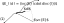
\includegraphics[width=0.25\textwidth]{img/2.png}
    %\caption{}
    %\label{fig:}
\end{figure}

\noindent
Из этих уравнений легко получить, что
\begin{equation}
    \left\{\begin{aligned}
        \frac{\partial U}{\partial z} &= - \frac{L_0}{c^2} \frac{d I}{d t} \\
        \frac{\partial I}{\partial z} &= - C_0 \frac{\partial U}{\partial t} 
    \end{aligned}\right.
    \hspace{0.5cm} \Rightarrow \hspace{0.5cm} 
    \boxed{
        \frac{\partial^2 U}{\partial t^2}  = \frac{c^2}{L_0 C_0} - \frac{\partial^2 V}{\partial z^2} 
    }.
\end{equation}
Решение аналогично будем искать в виде
\begin{equation}
    V = f_1 (z - vt) + f_2 (z + vt),
    \hspace{0.5cm} \Rightarrow \hspace{0.5cm} 
    v = \frac{c}{\sqrt{L_0 C_0}}.
\end{equation}
Кстати, если это всё посчитать для коаксиального кабеля, то
\begin{equation*}
    L_0 = 2 \mu \ln \frac{R_2}{R_1} , \hspace{0.5cm} 
    C_0 = \frac{\varepsilon}{2 \ln \frac{R_2}{R_1} },
    \hspace{0.5cm} \Rightarrow \hspace{0.5cm} 
    v = \frac{c}{\sqrt{\mu \varepsilon}}.
\end{equation*}


\subsubsection*{Коэффициент стоячей волны (standing wave ratio)}
Коэффициент стоячей волны -- отношение наибольшего значения амплитуды напряжённости электрического или магнитного поля стоячей волны в пучностях линии передачи к амплитуде в узлах.
КСВ является мерой согласования нагрузки (например, антенны) с линией передачи.

Наибольшее и наименьшее значения амплитуды соответсвенно равны
\begin{equation*}
    A_{\text{max}} = A_{\text{inc}} + A_{\text{ref}}, \hspace{0.5cm} 
    A_{\text{min}} = A_{\text{inc}} - A_{\text{ref}},
    \hspace{0.5cm} \Rightarrow \hspace{0.5cm} 
    \text{КСВ} = \frac{A_{\text{inc}} + A_{\text{ref}}}{A_{\text{inc}} - A_{\text{ref}}} = 
    \frac{1 + |\Gamma|}{1 - |\Gamma|},
\end{equation*}
где $|\Gamma|$ -- коэффициент отражения.

\subsubsection*{Согласованная нагрузка}
Рассмотрим длинную линию, пусть в цепи 
\begin{equation*}
    U = U_0 \cos \left(\omega_0 t - kz\right),  \hspace{0.5cm} 
    I = I_0 \cos \left(\omega_0 t - kz\right).
\end{equation*}
Сделаем следующий трюк. Возьмем, и продолжим линию до бесконечности, от которой, очевидно, ничего не отразится. Соотвественно нас интересует поиск эквивалентного импеданса системы. 
\begin{align*}
    U^* = U_0 \exp\left(i(\omega_0 t - kz)\right) &= U_0 e^{ikz} e^{-i\omega_0 t}, \\
    I^* = I_0 \exp\left(i(\omega_0 t - kz)\right) &= I_0 e^{ikz} e^{-i\omega_0 t}.
\end{align*}
Подставив эти выражения в волновое уравнение, и получим
\begin{equation*}
    ik U^* = i \omega_0 I^*,
    \hspace{0.5cm} 
    Z^* = U^* / I^* = \frac{\omega_0}{k},
    \hspace{0.5cm} \Rightarrow \hspace{0.5cm} 
    R = \frac{1}{c} \sqrt{\frac{L_0}{C_0}},
    \text{\ \ --- \ \ \textit{согласованная нагрузка}}.
\end{equation*}
То есть при наличии такого сопротивления на конце линии не будет никакого отражения. 




\sbsnum{25}{Формулы гладкой замены переменных в интеграле Лебега от функции}
\subsubsection*{Уравнение непрерывности}
\begin{to_def}[Предмет рассмотрения]
	Ввиду макроскопического рассмотрения \textit{жидкости}(газы) в гидродинамике представлется как сплошная среда, то есть малый элемент объёма жидкости содержит ещё достаточно больше количество молекул, относительно межмолекулярного расстояния.
\end{to_def}

Для описания движения жидкости требуется задать распределение скорости жидкости $\vc{v} = \vc{v}(x,y,z,t)$ и какие-либо её две термодинамические величины, как, например, плотность и давление. Важно отметить, что все эти величины относятся не к отдельной частице, а к точке в пространстве в определенное время.

\begin{to_thr}[Уравнение непрерывности]
\phantom{239}

\begin{proof}[$\triangle$]
	В маленьком объёме $V_{0}$ количество жидкости есть $\int_{V_0} \rho d V$.
	Через элемент поверхности, ограничивающей $V_0$, в единицу времени протекает $\rho \vc{v} \cdot d \vc{f}$ жидкости --- положительно или отрицательное число, в зависимости от того, вытекает или втекает жидкость соответственно.
	Тогда приравниваем для вытекания жидкости два наших рассуждения:
	\begin{equation*}
		- \frac{\partial}{\partial t} \int \rho d V =  \oint \rho \vc{v} \cdot d \vc{f}
		\hspace*{0.5 cm} 
		\Rightarrow 
		\hspace*{0.5 cm}
		\int \left(\frac{\partial \rho}{\partial t} + \div \rho \vc{v}\right)d V = 0
		\hspace*{0.5 cm}
		\Rightarrow
		\hspace*{0.5 cm}
		\frac{\partial \rho}{\partial t} + \div \rho \vc{v} = 0.
	\end{equation*}
	Последнее следует из того, что равенство должно иметь для любого объёма, таким образом получили искомое \textit{уравнение непрерывности}.
\end{proof}
	
\end{to_thr}

\subsubsection*{Уравнение Эйлера}

\begin{to_thr}[Уравнение Эйлера]
\phantom{239}

\begin{proof}[$\triangle$]
	Выделим в жидкости некоторый объём, полная сила, действующая на этот объём: $- \oint p d \vc{f} = - \int \grad p d V$, где интеграл из взятого по поверхности объёма преобразуется в сам рассматриваемый объём.
	Таким образом получили, что на единицу объёма жидкости будет действовать сила:
	\begin{equation*}
		\rho \frac{d \vc{v}}{d t} = - \grad p.
	\end{equation*}
	Однако стоящая здесь скорость определяет изменение скорости именно элемента объёма, а не точки в пространстве.
	Запишем это изменение скорости:
	\begin{equation*}
		d \vc{v} 
		=
		 \frac{\partial \vc{v}}{\partial t} d t + \frac{\partial \vc{v}}{\partial x^i} d x^i 
		= 
		\frac{\partial \vc{v}}{\partial t} d t + (d \vc{r} \cdot \nabla) \vc{v}
		\hspace*{1 cm}
		\Rightarrow
		\hspace*{1 cm}
		\frac{\partial \vc{v}}{\partial t} + (\vc{v} \nabla) \vc{v} = - \frac{1}{\rho} \grad p.
	\end{equation*}
	Последнее и есть искомое уравнение Эйлера.
\end{proof}
\end{to_thr}

Если же жидкость движется во внешнем поле тяжести, то, на каждый элемент объёма будет действовать сила, которая просто добавится к изначальному уравнению: 
\begin{equation*}
	\frac{\partial \vc{v}}{\partial t} + (\vc{v} \nabla) \vc{v} = - \frac{\nabla p}{\rho} + \vc{g}.
\end{equation*}

\subsubsection*{Уравнение Навье-Стокса}

Чтобы нормально учесть вязкость, нужно поговорить про \textit{поток импульса}.
Импульс единицы объёма жидкости есть $\rho \vc{v}$, скорость изменения его компоненты:
\begin{equation*}
	\frac{\partial}{\partial t} \rho v^i = \rho \frac{\partial v^i}{\partial t} + \frac{\partial \rho}{\partial t} v^i.
\end{equation*}
Уравнения непрерывности и Эйлера запишутся в тензорном виде:
\begin{equation*}
	\frac{\partial \rho}{\partial t} = - \frac{\partial (\rho v^k)}{\partial x^k},
	\hspace*{0.5 cm}
	\hspace*{0.5 cm}
	\frac{\partial v^i}{\partial t} = - v^k \frac{\partial v^i}{\partial x^k} - \frac{1}{\rho} \delta^{i k} \frac{\partial p}{\partial x^k}.
\end{equation*}
Тогда получим:
\begin{equation*}
	\frac{\partial}{\partial t} \rho v^i 
	= 
	- \rho v^k \frac{\partial v^i}{\partial x^k} -  \delta^{i k} \frac{\partial p}{\partial x^k} - v^i \frac{\partial \rho v^k}{\partial x^k} 
	=
	-\delta^{i k} \frac{\partial p}{\partial x^k} - \frac{\partial}{\partial x^k} \rho v^i v^k
	= - \frac{\partial \Pi^{i k}}{\partial x^k}.
\end{equation*}
\begin{to_def}
	$\Pi^{i k} $ --- \textit{тензор плотности потока импульса}:
	$
		\Pi^{i k} = p \delta^{i k} + \rho v^i v^k.
	$
\end{to_def}

Таким образом уравнение Эйлера у нас записалось в виде:
$
	\frac{\partial}{\partial t} \rho v^i = - \frac{\partial \Pi^{i k}}{\partial x^k}.
$
Поток импульса представляет собой чисто обратимый перенос импульса, связанный с просто механическим передвижением различных участков жидкости и с действующими в жидкости силами давления.
\textit{Вязкость} (внутреннее трение) жидкости проявляется в наличии ещё дополнительного, необратимого переноса импульса из мест с большой скоростью в места с меньшей.

Поэтому уравнение движения вязкой жидкости можно получить, прибавив к идеальному потоку импульса дополнительный член $\sigma^{i k}_{visc}$, определяющий такой вязкий перенос:
$
\Pi^{i k} = p \delta^{i k} + \rho v^i v^k - \sigma^{i k}_{visc} = - \sigma^{i k} + \rho v^i v^k.
$
\begin{to_def}
	Таким образом: $\sigma^{i k} = - p \delta^{i k} + \sigma^{i k}_{visc}$ называют \textit{тензором напряжений}, а $\sigma^{i k}_{visc}$ --- вязким тензором напряжений.
\end{to_def}

Чтобы написать выражение для вязкого напряжения сделаем пару оговорок. 
\textit{Во первых}, градиенты скорости движения участков жидкости относительно друг друга не велики, тогда $\sigma^{i k}_{visc}$ зависит лишь от первых производных скорости по координатам, линейно. \textit{Во вторых}, не зависящие от первых производных величины должны обращаться в нуль как для скорости потока $\vc{v} = \const$ и тензор должен быть нулевым. \textit{В третьих}, $\sigma^{i k}_{visc} = 0$ когда жидкость совершает целое равномерное вращение, поскольку никакого внутреннего трения тогда не будет.
Для такого равномерного вращения с $\vc{v} = [\vc{\omega} \vc{r}]$ линейными комбинациями производных обращающимися в нуль будут: $\frac{\partial v^i}{\partial x^k} + \frac{\partial v^k}{\partial x^i}$.

Это всё даёт нам мотивацию для не шибко сильных потоков несжимаемой жидкости согласится с Сэром Исааком Ньютоном, и написать тензор вязкого напряжения, как \textit{тензор скорости деформации}:
\begin{equation*}
	\sigma^{i k}_{visc} = \eta \left(\frac{\partial v^i}{\partial x^k} + \frac{\partial v^k}{\partial x^i}\right),
	\hspace*{1 cm}
	\Rightarrow
	\hspace*{1 cm}
	\sigma^{i k} = - p \delta^{i k} + \eta \left(\frac{\partial v^i}{\partial x^k} + \frac{\partial v^k}{\partial x^i}\right).
\end{equation*}
А уравнение Эйлера тогда для несжимаемой жидкости запишется:
\begin{equation*}
	\rho \left(\frac{\partial v^i}{\partial t} + v^k \frac{\partial v^i}{\partial x^k}\right)
	=
	- \delta^{i k} \frac{\partial p}{\partial x^k} + \frac{\partial}{\partial x^k} \left[\eta \left(\frac{\partial v^i}{\partial x^k} + \frac{\partial v^k}{\partial x^i}\right)\right].
\end{equation*}
а в более человеческом, привычном глазу, виде \textit{уравнение Навье-Стокса для несжимаемой жидкости}:
\begin{equation*}
	\frac{\partial \vc{v}}{\partial t} + (\vc{v} \triangle) \vc{v} = - \frac{1}{\rho} \grad p + \frac{\eta}{\rho} \Delta \vc{v}.
\end{equation*}
\begin{to_def}
	Коэффициент $\eta$ называется --- \textit{динамическим коэффициентом вязкости}, а отношение $\eta/\rho = \nu$ --- \textit{кинематической вязкостью}.
\end{to_def}


\newpage 


%%%%%%%%%%%%%%%%%%%%%%%%%%%%%%%%%%%%%%%%%%%%%%%%%%%%%%%%%%%%%%%%%%%%%%%%%%%%%%%%%%%
\section*{Многообразия (с краем) и формула Стокса}
\setcounter{section}{7}
\addcontentsline{toc}{section}{Многообразия (с краем) и формула Стокса}
%%%%%%%%%%%%%%%%%%%%%%%%%%%%%%%%%%%%%%%%%%%%%%%%%%%%%%%%%%%%%%%%%%%%%%%%%%%%%%%%%%%

\sbsnum{26}{Вложенные многообразия}
Напишем систему уравнений, соответствующую уравнениям Лагранжа первого рода:

\begin{equation}
    \sum_{\nu=1}^N \vc{a}_{\beta \nu} (\vc{r}_1, \ldots, \vc{r}_N, t) \cdot \vc{v}_\nu + a_\beta  (\vc{r}_1, \ldots, \vc{r}_N, t) = 0,
    \hspace{0.5cm} (\beta = 1, \ldots, s)
\end{equation}
$$
    f_\alpha (\vc{r}, t) = 0, \hspace{0.5cm} (\alpha = 1, \ldots, r),
$$
\begin{align}
    \sum_{\nu=1}^N \frac{\partial f_\alpha}{\partial \vc{r}_\nu} \cdot d \vc{r}_\nu + \frac{\partial f_\alpha}{\partial t} d t &= 0,
    \hspace{0.5cm} &(\alpha = 1, \ldots, r), \\
    \sum_{\nu=1}^N \vc{a}_{\beta\nu} \cdot d \vc{r}_\nu + a_\beta d t &= 0,
    \hspace{0.5cm} &(\beta = 1, \ldots, s).
\end{align}



Взяв выражения для виртуальных перемещений всегда можно получить силы реакции так называемым методом \textit{множителей Лагранжа}:
\begin{equation*}
    \sum_{\nu=1}^N \left(\vc{R}_\nu - \sum_{i = 1}^r \lambda_i \frac{\partial f_i}{\partial \vc{r}_\nu} - \sum_{j = 1}^s \mu_j \alpha_{j \nu}\right) \delta \vc{r}_\nu = 0
    \hspace*{1 cm}
    \Rightarrow
    \hspace*{1 cm}
    \vc{R}_\nu = \sum_{i = 1}^r \lambda_i \frac{\partial f_i}{\partial \vc{r}_\nu} + \sum_{j = 1}^s \mu_j \alpha_{j \nu}.
\end{equation*}
Полученные выражения для реакций идеальных сил через неопределенные множители Лагранжа $\lambda_i $ и $\mu_j $ можно подставить в исходное уравнение связей, получим \textit{уравнения Лагранжа первого рода}:
\begin{equation*}
    m_\nu \vc{w}_\nu = \vc{F}_\nu + \sum_{i = 1}^r \lambda_i \frac{\partial f_i}{\partial \vc{r}_\nu} + \sum_{j = 1}^s \mu_j \alpha_{j \nu}.
\end{equation*}

\newpage 

%%%%%%%%%%%%%%%%%%%%%%%%%%%%%%%%%%%%%%%%%%%%%%%%%%%%%%%%%%%%%%%%%%%%%%%%%%%%%%%%%%%
\section*{Решения (\textbf{BETA})}
\setcounter{section}{35}
\addcontentsline{toc}{section}{Решения}
%%%%%%%%%%%%%%%%%%%%%%%%%%%%%%%%%%%%%%%%%%%%%%%%%%%%%%%%%%%%%%%%%%%%%%%%%%%%%%%%%%%

\sbsnum{1}{Свёртка функций и её свойства}
Для точки $P$ движущейся относительно некоторого неподвижного тела (свяжем с ним точку $O$), можно ввести следующие характеристики:
\begin{to_def}[Радиус вектор, скорость и ускорение точки $P$]
	\begin{equation*}
	\vc{r} = \overrightarrow{O P},
	\hspace*{1 cm}
	\vc{v} = \frac{d \vc{r}}{d \vc{t}},
	\hspace*{1 cm}
	\vc{w} =  \frac{d \vc{v}}{d t} = \frac{d^2 \vc{r}}{d t^2}.
\end{equation*}	
\end{to_def}

\begin{to_def}
	Для задания движения точки, зная её траекторию, можно сопоставить ей дуговую координату $\sigma (t)$ и получить выражения для скорости и ускорения, выраженные в осях \textit{естественного трёхгранника} $\vc{\tau}, \vc{n}, \vc{b}$.
	Таким образом для $\vc{r} = \vc{r}(\sigma(t))$:
	\begin{equation*}
		\vc{\tau} (\sigma) = \frac{d \vc{r}}{d \sigma}, 
		\hspace*{1 cm} 
		\frac{d \vc{\tau}}{d \sigma} = \frac{1}{\rho} \vc{n} (\sigma),
	\end{equation*}
	где $\rho$ -- радиус кривизны. Для кривой в $\mathbb{R}^3$ добавим ещё вектор $b$ для правой тройки. Таким образом получим формулы Френе:
	\begin{equation*}
		\frac{d \vc{\tau}}{d s} = \frac{1}{\rho} \vc{n},
		\hspace*{1 cm}
		\frac{d \vc{n}}{d s} = - \frac{1}{\rho} \vc{\tau} + \varkappa \vc{b},
		\hspace*{1 cm}
		\frac{d \vc{b}}{d s} = - \varkappa \vc{n}.
	\end{equation*}
\end{to_def}

Таким образом сможем в компонентах трёхгранника выписать скорость и ускорение точки:
\begin{gather*}
   \vc{v} = \frac{d \vc{r}}{d t} = \frac{d \vc{r}}{d \sigma} \frac{d \sigma}{d t} = v_\tau \vc{\tau}
   \\
   \vc{w} = \frac{d \vc{v}}{d t} = \frac{d_\tau}{d t} \vc{\tau} + v_\tau \frac{d \vc{\tau}}{d \sigma} \frac{d \sigma}{d t} = \frac{d^2 \sigma}{d t^2} \vc{\tau} + \frac{v_\tau^2}{\rho} \vc{n}.
\end{gather*}
Как видно, ускорение точки представилось в видео $w = w_n + w_\tau $ --- \textit{нормальной} и \textit{тангенциальной} составляющей.

\begin{to_lem}[Из матана]
	Для $f_i \in  C^2 \colon U \mapsto V$, если $X$ -- касательный вектор в точке $p \in U$, то $X(f)$ можно определить как:
	\begin{equation*}
		X(f) = X(x^i) \frac{\partial f(p)}{\partial x^i}, \text{ а координаты этого вектора в криволинейных координатах: } X = X^i \frac{\partial}{\partial x^i}.
	\end{equation*}
\end{to_lem}

Каждую материальную точку можем определить $\vc{r}_1, \ldots, \vc{r}_N$ -- итого $\mathbb{R}^{3N}$. Но есть некоторые ограничения вида
\begin{equation*}
    f_i (\vc{r}, t) = 0.
\end{equation*}
Вложим в фазовое пространство многообразие $M$, в котором локально всё хорошо. Тогда
$\dim M = n$ -- число степеней свободы, а параметризация $q_1, \ldots, q_N$ -- криволинейные координаты. В каждой $A \in M$ верно, что $\dot{\vc{q}} \in TM_A$, то есть
\begin{equation*}
    TM = \bigcup_q T_qM \ni (q, \dot{q})
\end{equation*}

И так, движение точки можно задать, если её криволинейные координаты --- известне функции $q(t)$.
\begin{equation*}
	\vc{r} = \vc{r}(q_1, q_2, q_3) = x \vc{i} + y \vc{j} + z \vc{k}.
\end{equation*}

\begin{to_def}
	\textit{Коэффициентами Ламе} такие $H^i$. C их помощью удобно выразить единичные базисные векторы криволинейных координат: 
	\begin{equation*}
		H_i = \left|\frac{\partial \vc{r}}{\partial q^i} \right| = \sqrt{\left(\frac{\partial x}{\partial q^i}\right)^2 + \left(\frac{\partial y}{\partial q^i}\right)^2 + \left(\frac{\partial z}{\partial q^i}\right)^2}.
		\hspace*{1 cm}
		e^i = \frac{1}{H_i} \frac{\partial \vc{r}}{\partial q^i}.
	\end{equation*}
\end{to_def}

Далее будем координатными векторами называть $\vc{g}_i(\vc{r}) = \frac{\partial \vc{r}}{\partial q^i}$. Разложение произвольного вектора по локальному базису имеет вид:
\begin{equation*}
	\vc{a} = a^i \vc{g}_i = a_j \vc{g}^j.
\end{equation*}
Здесь $\vc{g}^j$ --- векторы двойственного базиса к базису из $\vc{g}_i$. В двойственном же (взаимном) базисе из матана мы видели:
\begin{equation*}
	X(f) = d f (X) = \partial_x f,
	\hspace*{1 cm}
	d x^i (\frac{\partial}{\partial x^j}) = \frac{\partial x^i}{\partial x^j} = \delta_j^i,
	\hspace*{1 cm}
	a = a_i d x^i.
\end{equation*}
Таким образом получаем скорость точки и её ковариантную компоненту:
\begin{equation*}
	\vc{v} = \frac{d \vc{r}}{d t} = \frac{\partial \vc{r}}{\partial q^i} \frac{d q^i}{d t} = \vc{g}_i \dot{q}^i,
	\hspace*{1 cm}
	v^i = \vc{q}^i.
\end{equation*}
И для ускорения:
\begin{equation*}
	w_k = \left(\frac{d \vc{v}}{d t}\right)_k = \frac{(d \vc{v})_k}{d t} = g_{k j} \frac{d v^j}{d t} + \Gamma_{k i j} v^j v^i.
\end{equation*}


\sbsnum{2}{Бесконечно гладкие функции с компактным носителем}
\begin{to_def}
	\textit{Твёрдое телое} --- множество точек, расстояние между которыми не меняется: $\forall j, j, t \colon \vc{|r}_i(t) - \vc{r}_j| = \const$. 
\end{to_def}

Точка $O$ это полюс. Во-первых перенесем начало координат в $O$. Введём систему координат $O_{\xi\nu\zeta}$ связанную с телом, -- тело относительно неё не движется
\begin{equation*}
	 \vc{r} = \vv{OA}, \, \vc{\rho} = \vv{OA} = \const \text{ в $O_{\xi\nu\zeta}$},
    \hspace{0.5cm} \Rightarrow \hspace{0.5cm} 
    \vc{r}(t) = R(t) \vc{\rho}.
\end{equation*}

\begin{wrapfigure}{r}{0.25\textwidth}
  \begin{center}
        \vspace{-10 mm}
        \includegraphics[width=0.9\linewidth]{img/eu_angles.png}
  \end{center}
    \caption{Углы Эйлера}
\end{wrapfigure}

Ортогональность матрицы $R$ даёт возможность описать её тремя независимыми параметрами. Один из вариантов сделать это -- углы Эйлера. 

Пусть начальная ПДСК $(x, y, z)$, а конечная -- $(X, Y, Z)$, при чём $xy \cap XY = ON$ -- линия узлов.
\begin{align*}
    1) \hspace{0.25cm}  \alpha &\colon Ox \to ON, &\text{ угол \textit{прецессии}}; \\
    2) \hspace{0.25cm}  \beta  &\colon Oz \to OZ, &\text{ угол \textit{нутации}}; \\
    3) \hspace{0.25cm}  \gamma &\colon OX \to ON, &\text{ угол \textit{собственного вращения}}.
\end{align*}
Повороты системы на эти углы называются прецессия, нутация и поворот на собственный угол (вращение). 

\phantom{42}

\noindent
Матричная запись углов Эйлера:
\begin{equation*}
    R_Z(\alpha) = \begin{pmatrix}
        \cos \alpha & - \sin \alpha & 0 \\
        \sin    a & \cos\alpha & 0 \\
        0 & 0 & 1\\
    \end{pmatrix},
\end{equation*}
\begin{equation*}
    R_X(\beta) = \begin{pmatrix}
        1 & 0 & 0 \\
        0 & \cos \beta & -\sin \beta \\
        0 & \sin \beta & \cos \beta \\
    \end{pmatrix},
    \hspace{1cm} 
    R_Z (\gamma) = \begin{pmatrix}
        \cos(\gamma) & - \sin \psi & 0 \\
        \sin \gamma & \cos \gamma & 0\\
        0 & 0 & 1
    \end{pmatrix}.
\end{equation*}

\begin{to_thr}[Теорема Эйлера]
     Произвольное перемещение твердого тела, имеющего неподвижную точку, можно осуществить посредством вращения вокруг некоторой оси, проходящей через эту точку. 
\end{to_thr}

\begin{to_thr}[Теорема Шаля]
     Самое общее перемещение твердого тела разлагается на поступательное перемещение, при котором произвольно выбранный полюс переходит из своего первоначального положения в конечное, и на вращение вокруг некоторой оси, проходящей через этот полюс. Это разложение можно совершить не единственным способом, выбирая за полюс различные точки тела; при этом направление и длина поступательного перемещения будут изменяться при выборе различных 
полюсов, а направление оси вращения и угол поворота вокруг нее не зависят от выбора полюса. 
\end{to_thr}

\begin{to_thr}[Теорема Моцци]
\label{thr_moz}
     Самое общее перемещение твердого тела является винтовым перемещением.
\end{to_thr}

\begin{to_con}[Теорема Бернулли-Шаля]
     Самое общее перемещение плоской фигуры в своей плоскости есть либо поступательное перемещение, либо вращение вокруг точки. Эта точка называется центром конечного вращения.
\end{to_con}

\sbsnum{3}{Приближение функций бесконечно гладкими}
Проведём два вектора $\vc{r}_A, \vc{r}_O$:
\begin{equation*}
    \vc{r}_A = \vc{r}_O + \vc{r} = \vc{r}_O + R(t) \vc{\rho}
    \hspace{0.5cm} \overset{d / dt}{\Rightarrow} \hspace{0.5cm} 
    \vc{v}_A = \vc{v}_O + \dot{R} \rho = \vc{v}_O + \dot{R} R^{-1}\vc{r}
\end{equation*}
но,
\begin{equation*}
    RR\T = E, \dot{R} R\T + R \dot{R}\T = 0, \dot{R} R\T = - R \dot{R}\T,
    (\dot{R} R^{-1})\T = - \dot{R} R^{-1}.
\end{equation*}

То есть $\dot{R} R^{-1}$ кососимметрична. Тогда пусть
\begin{equation*}
    \dot{R} R^{-1} = \Omega = \begin{pmatrix}
        0 & -\omega_z & w_y \\
        w_z & 0 & -\omega_x \\
        -\omega_y & \omega_x & 0\\
    \end{pmatrix}
\end{equation*}
Таким образом мы доказали следующую теорему.

\begin{to_thr}[формула Эйлера]
\label{eq_euler}
    Существует единственный вектор\footnote{
        Псевдоветор же, нет?
    } $\vc{\omega}$, называемый \textbf{угловой скоростью тела}, с помощью которого скорость $\vc{v}$ точки тела может быть представлена в виде
    \begin{equation*}
        \vc{v}_A = \vc{v}_O + \vc{\omega} \times \vc{r}
        \hspace{0.5cm} \text{--} \hspace{0.5cm} \text{\textbf{формула Эйлера}.}
    \end{equation*}
\end{to_thr}

Тогда, например, при постоянном радиус векторе верно, что
\begin{equation*}
    \vc{v}_A = \frac{d \vc{a}}{dt} = \vc{\omega} \times \vc{a},
    \hspace{0.5cm} \text{при условии $a = \const$}.
\end{equation*}

Можно вывести ускорение точки твёрдого тела
\begin{align*}
    \vc{\mathrm{w}}_A &= \vc{\mathrm{w}}_O + \frac{d \vc{\omega}}{dt} \times \vc{r} + \vc{\omega} \times \frac{d \vc{r}}{dt}, \\
    \vc{\mathrm{w}}_A &= \vc{\mathrm{w}}_O + \vc{\varepsilon} \times \vc{r} + \vc{\omega} \times \left(\vc{\omega} \times \vc{r} \right)
    \hspace{0.5cm} \text{--} \hspace{0.5cm} \text{\textbf{формула Ривальса},}
\end{align*}
где $\vc{\varepsilon} = d \vc{\omega} / d t$ -- \textit{угловое ускорение}.

\subsubsection*{Вращение вокруг неподвижной оси}
\begin{wrapfigure}{r}{0.25\textwidth}
  \begin{center}
        \vspace{-10 mm}
        \includegraphics[width=0.9\linewidth]{img/stable_axis.png}
  \end{center}
    \caption{Ориентация тела относительно неподвижной системы координат}
\end{wrapfigure}
Пусть точка $P$ задана в связанной системе координат радиус-вектором $\rho$:
\begin{equation*}
    \vc{r} = A \vc{\rho},
    \hspace*{0.5 cm}
    A = \begin{pmatrix}
            \cos \varphi & - \sin \varphi & 0 \\
            \sin \varphi & \cos \varphi & 0 \\
            0 & 0 & 1
        \end{pmatrix}.
\end{equation*}
После прямых вычислений получаем, что
\begin{equation*}
    \dot{A} A^{-1} = 
    \begin{pmatrix}
        0 & - \dot{\varphi} & 0 \\
        \dot{\varphi} & 0 & 0 \\
        0 & 0 & 0    
    \end{pmatrix},
    \hspace*{1 cm}
    \dot{\omega} = \begin{pmatrix}
        0 \\ 0 \\ \dot{\varphi}
    \end{pmatrix},
    \hspace*{1 cm}
    \vc{\varepsilon} = \begin{pmatrix}
        0 \\ 0 \\ \ddot{\varphi}    
    \end{pmatrix}.
\end{equation*}
Таким образом получили, что угловая скорость $\vc{\omega}$ направлена по оси вращения по правилу буравчика. Угловое ускорение $\vc{\varepsilon}$ коллинеарно $\vc{\omega}$.

Для вычисления $w_P$ примем $O$ за полюс. Тогда $v_O= 0$, что значит $\vc{v} = \vc{\omega} \times \vc{r}$ -- вектор скорости перпендикулярен оси вращения. И из формулы Ривальса:
\begin{equation*}
    w = \underbrace{\vc{\varepsilon} \times \vc{r}}_{w_\text{вр}} + \underbrace{\vc{\omega} \times \vc{v}}_{w_\text{ос}},
    \hspace*{1 cm}
\end{equation*}
где \textit{вращательное} ускорение $w_\text{вр} = \ddot{|\varphi}| d$, а \textit{осестремительное} $w_\text{ос} = \omega^{2}d$, а $d$ --- радиус окружности, по которой движется $P$.

\subsubsection*{Движение вокруг неподвижной точки}
Точка $O$ --- неподвижна, тогда $v_0 = 0, \ w_0 = 0 $ и формулы, полученные в разделе выше одни и те же. Однако стоит ввести пару определений:
\begin{to_def}
    \textit{Мгновенная ось вращения} --- ось на которой в данный момент времени лежит $\vc{\omega}$, которая в свою очередь --- \textit{мгновенная угловая скорость}. 
\end{to_def}
\begin{to_def}
    При своём движении мгновенная ось вращения описывает в теле коническую поверхность --- \textit{подвижный аксоид}, а в абсолютном пространстве --- \textit{неподвижный аксоид}.
    При движении тела подвижный аксоид катится по неподвижному без скольжения.
\end{to_def}

Годограф $\vc{\omega}$ лежит на неподвижном аксоиде. 
Так как $\vc{\varepsilon} = \vc{\dot{\omega}}$, то $\vc{\varepsilon}$ направлено по касательной к годографу и вовсе не обязательно по мгновенной оси вращения. 
Если $\vc{\omega} = \omega \vc{e}$, для единичного $\vc{e}$, то $\vc{\varepsilon} = \dot{\omega} \vc{e} +\omega \vc{\dot{e}}$.
Если мгновенная ось вращается вокруг $O$ с $\vc{\Omega}$, то $\omega \vc{\dot{e}} = \vc{\Omega} \times \vc{\omega}$.

Вновь воспользовавшись формулой Ривальса вычислим осетремительное ускорение, для $Q$ --- точке на мгновенной оси вращения:
\begin{equation*}
    w_\text{ос} = \vc{\omega}\times (\vc{\omega} \times \vc{r}) = \omega^2 \vc{e} \times (\vc{e} \times \vc{r}) = \omega^2[\vc{e} (\vc{e} \cdot \vc{r}) - \vc{r}] = \omega^2 (\overrightarrow{O Q} - \vc{r}) = \omega^2 \vc{l}.
\end{equation*}
Таким образом получили, что $w_\text{ос}$ совпадает при вращении, как если бы ось было неподвижной.

\subsubsection*{Плоское движение}
\begin{to_def}
    \textit{Плоское движение} --- движение тела, при котором все его точки перемещаются в плоскостях параллельных некоторой неподвижной плоскости.
\end{to_def}

Плоская фигура вынужденно двигаясь в своей плоскости имеет три степени свободы: $(x,y,\varphi)$. Скорости и ускорения всё так же ищутся по общем формулам, но в данном случае полезно рассмотреть несколько теорем:
\begin{to_thr}
    При плоском движении фигуры во мгновение $t$, если движение не поступательно, то $\exists ! C$-точка, такая что $v_C =0$, а остальные точки тела движутся как при вращении вокруг $C$.
\end{to_thr}
\begin{to_def}
    Такая точка $C$ --- называется \textit{мгновенным центром скоростей}.
\end{to_def}

\begin{to_thr}
    Для движения плоской фигуры в своей плоскости. Если в момент $t$ $\dot{\varphi} \neq 0 || \ddot{\varphi} \neq 0$, то в $t$ $\exists ! Q$-точка фигуры, такая что $w_Q = 0$.
\end{to_thr}

\sbsnum{6}{Теоремы о системе неявных функций}
\begin{to_thr}[Теорема о неявной функции]
\label{thr_6.32}
     Пусть функции $f_1, \ldots, f_k$ непрерывно дифференцируемы в окрестности $p \in \mathbb{R}^n$ и 
    \begin{equation*}
        \det \left(
            \frac{\partial f_i}{\partial x_j} 
        \right) \neq 0
    \end{equation*}
    в этой окрестности. Пусть $f_i(p) = y_i$, $i = 1, \ldots, k$. Тогда найдётся окрестность точки $p$ вида $U \times V$, $U \subset \mathbb{R}^k$, $V \subset \mathbb{R}^{n-k}$, такая что в этой окрестности множество решений системы уравнений
    \begin{equation*}
        \left\{\begin{aligned}
            f_1(x) &= y_1, \\
            &\ldots \\
            f_k(x) &= y_k,
        \end{aligned}\right.
    \end{equation*}
    совпадает с графиком непрерывно дифференцируемого отображения $\varphi \colon V \to U$, заданного в координатах как
    \begin{equation*}
        \left\{\begin{aligned}
            x_1 &= \varphi_1 (y_1, \ldots, y_k,\ x_{k+1}, \ldots, x_n),\\
            &\ldots\\
            x_k &= \varphi_k (y_1, \ldots, y_k,\ x_{k+1}, \ldots, x_n),
        \end{aligned}\right.
    \end{equation*}
    то есть отображения $\mathbb{R}^{n-k} \mapsto \mathbb{R}^k$.
\end{to_thr}




\newpage
%%%%%%%%%%%%%%%%%%%%%%%%%%%%%%%%%%%%%%%%%%%%%%%%%%%%%%%%%%%%%%%%%%%%%%%%%%%%%%%%%%%
\section*{Призраки прошлого и настоящего}
\setcounter{section}{36}
\addcontentsline{toc}{section}{Призраки прошлого и настоящего}
%%%%%%%%%%%%%%%%%%%%%%%%%%%%%%%%%%%%%%%%%%%%%%%%%%%%%%%%%%%%%%%%%%%%%%%%%%%%%%%%%%%
\sbsnum{239}{Прошлого}
\begin{to_thr}[Дифференцирование под знаком интеграла]
% \footnote{Функция $g \colon X \to \mathbb{R}^+$ и $g \in \L_c$}
\label{5.95}
    \begin{equation*}
    \begin{split}
    \left.
        \begin{aligned}
            &f(x, y) \in \L^x_c \; \forall y \in (a, b) \\
            &f \text{ дифференцируема по } y \\
            &\forall x \in X, \forall y \in (a, b) |f'_y(x, y)| \leq g(x) \\
            &g \geq 0 \colon X \to \mathbb{R}^+ \in L_c \text{ на } X
        \end{aligned}
    \right\} \hspace{1cm}
    \Rightarrow \hspace{1cm}
    \frac{d}{dy} \int_X f(x, y) \d x = \int_X f'_y (x, y) \d x.
    \end{split}
    \end{equation*}
\end{to_thr}

\begin{to_thr}
\label{thr_5.75}
    Пусть функция $f \colon \mathbb{R}^n \to \mathbb{R}$ интегрируема по Лебегу с конечным интегралом. Тогда $f$ можно сколь угодно близко приблизить в среднем элементарно ступенчатой функцией.
\end{to_thr}


\begin{to_thr}[Неравенство Коши-Буняковского]
\label{thr_5.94}
     Пусть функции $f, g \colon X \mapsto \mathbb{R}$ измеримы по Лебегу и их квадраты $|f|^2, \ |g|^2$ имеют конечные интегралы. Тогда
     \begin{equation*}
         \left(
            \int_X f(x) g(x) \d x
         \right)^2 \leq
         \left(
            \int_X |f(x)|^2 \d x
         \right) \cdot 
         \left(
            \int_X |g(x)|^2 \d x
        \right).
     \end{equation*}
\end{to_thr}

\sbsnum{566}{Настоящего}
\begin{to_tas}[Замена координат в интеграле для собственных отображений вообще]
    \label{task_6.108}
    Пусть гладкое отображение $\varphi \colon \mathbb{R}^n \mapsto \mathbb{R}^n$ является собственным. Тогда
    \begin{equation*}
        \int_{\mathbb{R}^n}\varphi^* \nu = C_\varphi \int_{\mathbb{R}^n} \nu, \hspace{0.5cm} 
        C_\varphi \in \mathbb{Z}.
    \end{equation*}
\end{to_tas}

\subsubsection*{Формула Стокса}


\begin{to_lem}[формула Стокса в узком смысле]
     Для компактной двумерной поверхности с краем (то есть вложенного двумерного многообразия с краем) $S \subset \mathbb{R}^3$ верна
\begin{equation*}
    \int_{\partial S} P \d x + Q \d y + R \d z =
    \int_S \left(\frac{\partial R}{\partial y} - \frac{\partial Q}{\partial z} \right) \d y \wedge d z + 
    \left(\frac{\partial P}{\partial z} - \frac{\partial R}{\partial x} \right) \d z \wedge dx + 
    \left(\frac{\partial Q}{\partial x} - \frac{\partial P}{\partial y} \right) \d x \wedge \d y.
\end{equation*}
\end{to_lem}


\begin{to_tas} 
    Площадь области, ограниченной замкнутой гладкой кривой без самопересечений $C \subset \mathbb{R}^2$, можно посчитать по формуле:
    \begin{equation*}
         A = \pm \int_C x \d y,
     \end{equation*} 
    где знак выбирается в зависимости от ориентации кривой.
\end{to_tas}

\begin{to_tas} 
    Объём области в $\mathbb{R}^3$, ограниченной связной вложенной компактной поверхностью без края $S \subset \mathbb{R}^3$, можно посчитать по формуле:
    \begin{equation*}
         A = \pm \int_S x \d y \wedge d z,
     \end{equation*} 
    где знак выбирается в зависимости от ориентации поверхности.
\end{to_tas}

\newcommand{\dmat}[4]{
  \ifthenelse{
    \equal{#1}{3}
  }{
\begin{pmatrix}
    #2 & 0 & 0 \\
    0 & #3 & 0 \\
    0 & 0 & #4 \\
\end{pmatrix}
  }{
  \ifthenelse{
      \equal{#1}{2}
    }{
  \begin{pmatrix}
      #2 & 0 \\
      0 & #3 \\
  \end{pmatrix}
    }{
      \text{\textcolor{red}{error}}
    }
  }
}

\newcommand{\skmat}[4]{
  \ifthenelse{
    \equal{#1}{3}
  }{
\begin{pmatrix}
    0 & -#4 & #3 \\
    #4 & 0 & -#2 \\
    -#3 & #2 & 0 \\
\end{pmatrix}
  }{
  \ifthenelse{
      \equal{#1}{2}
    }{
  \begin{pmatrix}
      0 & #2 \\
      -#2 & 0 \\
  \end{pmatrix}
    }{
      \text{\textcolor{red}{error}}
    }
  }
}
\usepackage[T2A]{fontenc}                   %!? закрепляет внутреннюю кодировку LaTeX
\usepackage[utf8]{inputenc}                 %!  закрепляет кодировку utf8
\usepackage[english,russian]{babel}         %!  подключает русский и английский
\usepackage[margin=1.7cm]{geometry}         %!  фиксирует оступ на 2cm

\usepackage[unicode, pdftex]{hyperref}      %!  оглавление для панели навигации по PDF-документу + гиперссылки

\usepackage{amsthm}                         %!  newtheorem и их сквозная нумерация
\usepackage{hypcap}                         %?  адресация на картинку, а не на подпись к ней
\usepackage{caption}                        %-  позволяет корректировать caption 
\usepackage{fancyhdr}                       %   добавить верхний и нижний колонтитул
\usepackage{wrapfig}                        %!  обтекание таблиц и рисунков

\usepackage{amsmath}                        %!  |
\usepackage{amssymb,textcomp, esvect,esint} %!  |важно для формул 
\usepackage{amsfonts}                       %!  математические шрифты
\usepackage{mathrsfs}                       %  добавит красивые E, H, L
\usepackage{ulem}                           %!  перечеркивание текста
\usepackage{abraces}                        %?  фигурные скобки сверху или снизу текста
\usepackage{pifont}                         %!  нужен для крестика
\usepackage{cancel}                         %!  аутентичное перечеркивание текста
\usepackage{esvect}                         %  добавит вектора стрелочками

\usepackage{graphicx}                       %?  графическое изменение текста
\usepackage{indentfirst}                    %   добавить indent перед первым параграфом
\usepackage{xcolor}                         %   добавляет цвета
\usepackage{enumitem}                       %!  задание макета перечня.

\usepackage{booktabs}                       %!  добавляет книжные линии в таблицы
\usepackage{multirow}                       %   объединение ячеек в таблицах

\usepackage{tikz}                           %!  высокоуровневые рисунки (кружочек)

\usepackage{import}                         %   |
\usepackage{xifthen}                        %   |
\usepackage{pdfpages}                       %   | вставка рисунков pdf_tex
\usepackage{transparent}                    %   |

\setlength{\headheight}{12.52pt}            % избегать warning

\usepackage{chngcntr}
\renewcommand\thesubsection{\arabic{subsection}}
\counterwithout{equation}{section}% file's preambule
%%%%%%%%%%%%%%%%%%%



% connect packages
\usepackage[T2A]{fontenc}
\usepackage[utf8]{inputenc}
\usepackage[english]{babel}
\usepackage{hyperref}     % ТАК_НУЖНО
\hypersetup{unicode=true} % ТАК_НУЖНО
\usepackage{amsmath}
\usepackage{amssymb,textcomp, esvect,esint}
\usepackage{amsfonts}
\usepackage{amsthm}
\usepackage{graphicx}
\usepackage{indentfirst}
\usepackage{xcolor}
\usepackage{enumitem}
\usepackage{booktabs}
\usepackage{caption}
\usepackage{listings}
\usepackage{tikz}

\usepackage{esvect}
\usepackage{movie15}
\usepackage{animate}

% create environment

\newtheorem{to_thr}{Thr}[subsection]
\newtheorem{to_suj}[to_thr]{Suj}
\newtheorem{to_lem}[to_thr]{Lem}
\newtheorem{to_com}[to_thr]{Com}
\newtheorem{to_con}[to_thr]{Con}
\theoremstyle{definition}
\newtheorem{to_def}[to_thr]{Def}


\newenvironment{itemize*}
{
    \begin{itemize}
        \setlength{\itemsep}{1pt}
        \setlength{\parskip}{1pt}}
    {\end{itemize}
}

\newenvironment{enumerate*}
{
    \begin{enumerate}
        \setlength{\itemsep}{1pt}
        \setlength{\parskip}{1pt}}
    {\end{enumerate}
}

\newenvironment{description*}
{
    \begin{description}
        \setlength{\itemsep}{1pt}
        \setlength{\parskip}{1pt}}
    {\end{description}
}

% document palette

\definecolor{grey}{HTML}{666666}
\definecolor{linkcolor}{HTML}{0000CC}
\definecolor{urlcolor}{HTML}{006600}
\hypersetup{
    pdfstartview=FitH,  
    linkcolor=linkcolor,
    urlcolor=urlcolor, 
    colorlinks=true,
    citecolor=blue}

% add (renew) commands
% add (renew) commands

\renewcommand{\Im}{\mathop{\mathrm{Im}}\nolimits}
\renewcommand{\Re}{\mathop{\mathrm{Re}}\nolimits}
\renewcommand{\d}{\, d}
\renewcommand{\leq}{\leqslant}
\renewcommand{\geq}{\geqslant}
\renewcommand{\L}{\mathcal{L}}


\newcommand{\vc}[1]{\mbox{\boldmath $#1$}}
\newcommand{\T}{^{\text{T}}}

\newcommand{\incfig}[1]{%
    \def\svgwidth{\columnwidth}
    \import{./figures/}{#1.pdf_tex}
}

\newcommand{\diag}{\mathop{\mathrm{diag}}\nolimits}
\newcommand{\id}{\mathop{\mathrm{id}}\nolimits}
\newcommand{\grad}{\mathop{\mathrm{grad}}\nolimits}
\renewcommand{\div}{\mathop{\mathrm{div}}\nolimits}
\newcommand{\rot}{\mathop{\mathrm{rot}}\nolimits}
\newcommand{\Ker}{\mathop{\mathrm{Ker}}\nolimits}
\newcommand{\Spec}{\mathop{\mathrm{Spec}}\nolimits}
\newcommand{\sign}{\mathop{\mathrm{sign}}\nolimits}
\newcommand{\tr}{\mathop{\mathrm{tr}}\nolimits}
\newcommand{\rg}{\mathop{\mathrm{rg}}\nolimits}

\newcommand{\const}{\text{const}}
\newcommand{\red}[1]{\textcolor{red}{#1}}
\newcommand{\xmark}{\ding{55}}

\newcommand{\sbsnum}[2]{
    \setcounter{subsection}{\the\numexpr #1 - 1 \relax}
    \subsection{#2}
}
\newcommand{\secnum}[2]{
    \section*{#2}
    \setcounter{section}{#1}
    \addcontentsline{toc}{section}{#2}
}


\newcommand{\set}[2]{{#1}^{1}, \ldots, {#1}^{#2}}

\catcode`\^ = 13 \def^#1{\sp{#1}{}} % чтобы штрих нормально работал

% add page header
% add page header

\pagestyle{fancy}
\fancyhf{}
% \fancyhead[RE,LO]{\textsc{Ф\raisebox{-1.5pt}{и}з\TeX}}
\fancyhead[LE,RO]{Ж\raisebox{-1.5pt}{и}К}
% \fancyhead[CO,CE]{\leftmark}
\fancyfoot[LE,RO]{\textcolor{grey}{\texttt{\thepage}}}



% matrixes shortcuts 
\newcommand{\dmat}[4]{
  \ifthenelse{
    \equal{#1}{3}
  }{
\begin{pmatrix}
    #2 & 0 & 0 \\
    0 & #3 & 0 \\
    0 & 0 & #4 \\
\end{pmatrix}
  }{
  \ifthenelse{
      \equal{#1}{2}
    }{
  \begin{pmatrix}
      #2 & 0 \\
      0 & #3 \\
  \end{pmatrix}
    }{
      \text{\textcolor{red}{error}}
    }
  }
}

\newcommand{\skmat}[4]{
  \ifthenelse{
    \equal{#1}{3}
  }{
\begin{pmatrix}
    0 & -#4 & #3 \\
    #4 & 0 & -#2 \\
    -#3 & #2 & 0 \\
\end{pmatrix}
  }{
  \ifthenelse{
      \equal{#1}{2}
    }{
  \begin{pmatrix}
      0 & #2 \\
      -#2 & 0 \\
  \end{pmatrix}
    }{
      \text{\textcolor{red}{error}}
    }
  }
}

% additional symbols and commands


\DeclareRobustCommand{\tmpsim}{ %%%%%%%%%%%%%% ~ < %%%%%%%%%%%%%%%%%%%
  \mathbin{\text{
      \raisebox{-1pt}{
            \hspace{-4.5pt} \rotatebox{-26}{\scalebox{0.8}[0.7]{$\sim$}}
        }
  }}
}
\def\lesim{{
    \setbox0\hbox{$\ <\ $}
    \rlap{\hbox to \wd0{\hss$\tmpsim$\hss}}\box0
}}
%%%%%%%%%%%%%%%%%%%%%%%%%%%%%%%%%%%%%%%%%%%%%%%%%%%%%%%%%%%%%%%%%%%%%%


\def\letuscom{%%%%%%%%%%%%%%%%%%%%%% ПУСТЬ %%%%%%%%%%%%%%%%%%%%%%%%%%
\mathord{\setbox0=\hbox{$\exists$}%
     \hbox{\kern 0.125\wd0%
           \vbox to \ht0{%
              \hrule width 0.75\wd0%
              \vfill%
              \hrule width 0.75\wd0}%
           \vrule height \ht0%
           \kern 0.125\wd0}%
   }%
}
\newcommand{\letus}{\raisebox{-1.2pt}{$\letuscom$}}
%%%%%%%%%%%%%%%%%%%%%%%%%%%%%%%%%%%%%%%%%%%%%%%%%%%%%%%%%%%%%%%%%%%%%%


\usepackage{arydshln} %%%%%%%%%%%%%%% ЛИНИИ В МАТРИЧКЕ %%%%%%%%%%%%%%%
\makeatletter
  \renewcommand*\env@matrix[1][*\c@MaxMatrixCols c]{%
    \hskip -\arraycolsep
    \let\@ifnextchar\new@ifnextchar
  \array{#1}}
\makeatother
%%%%%%%%%%%%%%%%%%%%%%%%%%%%%%%%%%%%%%%%%%%%%%%%%%%%%%%%%%%%%%%%%%%%%%


\makeatletter %%%%%%%%%%%%%%% КРУЖОЧЕК %%%%%%%%%%%%%%%%%%%%%%%%%%%%%%%
\newcommand*{\encircled}[1]{\relax\ifmmode\mathpalette
\@encircled@math{#1}\else\@encircled{#1}\fi}
\newcommand*{\@encircled@math}[2]{\@encircled{$\m@th#1#2$}}
\newcommand*{\@encircled}[1]{%
  \tikz[baseline,anchor=base]{\node[draw,circle,outer sep=0pt,
                                        inner sep=.2ex] {#1};}}
\makeatother
%%%%%%%%%%%%%%%%%%%%%%%%%%%%%%%%%%%%%%%%%%%%%%%%%%%%%%%%%%%%%%%%%%%%%%


\makeatletter
\def\upintkern@{\mkern-7mu\mathchoice{\mkern-3.5mu}{}{}{}}
\def\upintdots@{\mathchoice{\mkern-4mu\@cdots\mkern-4mu}%
 {{\cdotp}\mkern1.5mu{\cdotp}\mkern1.5mu{\cdotp}}%
 {{\cdotp}\mkern1mu{\cdotp}\mkern1mu{\cdotp}}%
 {{\cdotp}\mkern1mu{\cdotp}\mkern1mu{\cdotp}}}
\newcommand{\upiint}{\DOTSI\protect\UpMultiIntegral{2}}
\newcommand{\upiiint}{\DOTSI\protect\UpMultiIntegral{3}}
\newcommand{\upiiiint}{\DOTSI\protect\UpMultiIntegral{4}}
\newcommand{\upidotsint}{\DOTSI\protect\UpMultiIntegral{0}}
\newcommand{\UpMultiIntegral}[1]{%
  \edef\ints@c{\noexpand\upintop
    \ifnum#1=\z@\noexpand\upintdots@\else\noexpand\upintkern@\fi
    \ifnum#1>\tw@\noexpand\upintop\noexpand\upintkern@\fi
    \ifnum#1>\thr@@\noexpand\upintop\noexpand\upintkern@\fi
    \noexpand\upintop
    \noexpand\ilimits@
  }%
  \futurelet\@let@token\ints@a
}
\makeatother

\DeclareFontFamily{OMX}{mdbch}{}
\DeclareFontShape{OMX}{mdbch}{m}{n}{ <->s * [0.8]  mdbchr7v }{}
\DeclareFontShape{OMX}{mdbch}{b}{n}{ <->s * [0.8]  mdbchb7v }{}
\DeclareFontShape{OMX}{mdbch}{bx}{n}{<->ssub * mdbch/b/n}{}

\DeclareSymbolFont{uplargesymbols}{OMX}{mdbch}{m}{n}
\SetSymbolFont{uplargesymbols}{bold}{OMX}{mdbch}{b}{n}
\DeclareMathSymbol{\upintop}{\mathop}{uplargesymbols}{82}
\DeclareMathSymbol{\upointop}{\mathop}{uplargesymbols}{"48}

\DeclareFontEncoding{MDB}{}{}
\DeclareFontFamily{MDB}{mdbch}{}
\DeclareFontShape{MDB}{mdbch}{m}{n}{ <->s * [0.8]  mdbchrmb }{}
\DeclareFontShape{MDB}{mdbch}{b}{n}{ <->s * [0.8]  mdbchbmb }{}
\DeclareFontShape{MDB}{mdbch}{bx}{n}{<->ssub * mdbch/b/n}{}
\DeclareFontSubstitution{MDB}{cmr}{m}{n}
\DeclareSymbolFont{mathdesignB}{MDB}{mdbch}{m}{n}%
\SetSymbolFont{mathdesignB}{bold}{MDB}{mdbch}{b}{n}%
\DeclareMathSymbol{\upintclockwise}{\mathop}{mathdesignB}{128}
\DeclareMathSymbol{\upointclockwise}{\mathop}{mathdesignB}{130}
\DeclareMathSymbol{\upointctrclockwise}{\mathop}{mathdesignB}{132}
\DeclareMathSymbol{\upoiint}{\mathop}{mathdesignB}{134}
\DeclareMathSymbol{\upoiiint}{\mathop}{mathdesignB}{136}

\makeatletter
\renewcommand{\int}{\DOTSI\upintop\ilimits@}
\renewcommand{\oint}{\DOTSI\upointop\ilimits@}
\makeatother









% set skip of equation length 

\setlength{\abovedisplayskip}{3pt}
\setlength{\abovedisplayshortskip}{3pt}
\setlength{\belowdisplayskip}{3pt}
\setlength{\belowdisplayshortskip}{3pt}

\numberwithin{equation}{section}

\DeclareRobustCommand{\tmpsim}{ %%%%%%%%%%%%%% ~ < %%%%%%%%%%%%%%%%%%%
  \mathbin{\text{
      \raisebox{-1pt}{
            \hspace{-4.5pt} \rotatebox{-26}{\scalebox{0.8}[0.7]{$\sim$}}
        }
  }}
}
\def\lesim{{
    \setbox0\hbox{$\ <\ $}
    \rlap{\hbox to \wd0{\hss$\tmpsim$\hss}}\box0
}}
%%%%%%%%%%%%%%%%%%%%%%%%%%%%%%%%%%%%%%%%%%%%%%%%%%%%%%%%%%%%%%%%%%%%%%


\def\letuscom{%%%%%%%%%%%%%%%%%%%%%% ПУСТЬ %%%%%%%%%%%%%%%%%%%%%%%%%%
\mathord{\setbox0=\hbox{$\exists$}%
     \hbox{\kern 0.125\wd0%
           \vbox to \ht0{%
              \hrule width 0.75\wd0%
              \vfill%
              \hrule width 0.75\wd0}%
           \vrule height \ht0%
           \kern 0.125\wd0}%
   }%
}
\newcommand{\letus}{\raisebox{-1.2pt}{$\letuscom$}}
%%%%%%%%%%%%%%%%%%%%%%%%%%%%%%%%%%%%%%%%%%%%%%%%%%%%%%%%%%%%%%%%%%%%%%


\usepackage{arydshln} %%%%%%%%%%%%%%% ЛИНИИ В МАТРИЧКЕ %%%%%%%%%%%%%%%
\makeatletter
  \renewcommand*\env@matrix[1][*\c@MaxMatrixCols c]{%
    \hskip -\arraycolsep
    \let\@ifnextchar\new@ifnextchar
  \array{#1}}
\makeatother
%%%%%%%%%%%%%%%%%%%%%%%%%%%%%%%%%%%%%%%%%%%%%%%%%%%%%%%%%%%%%%%%%%%%%%


\makeatletter %%%%%%%%%%%%%%% КРУЖОЧЕК %%%%%%%%%%%%%%%%%%%%%%%%%%%%%%%
\newcommand*{\encircled}[1]{\relax\ifmmode\mathpalette
\@encircled@math{#1}\else\@encircled{#1}\fi}
\newcommand*{\@encircled@math}[2]{\@encircled{$\m@th#1#2$}}
\newcommand*{\@encircled}[1]{%
  \tikz[baseline,anchor=base]{\node[draw,circle,outer sep=0pt,
                                        inner sep=.2ex] {#1};}}
\makeatother
%%%%%%%%%%%%%%%%%%%%%%%%%%%%%%%%%%%%%%%%%%%%%%%%%%%%%%%%%%%%%%%%%%%%%%


